% shtthesis, an unofficial LaTeX thesis template for ShanghaiTech University.
% Copyright (C) 2021 Li Rundong <rundong.001@gmail.com>
%
% This program is free software: you can redistribute it and/or modify
% it under the terms of the GNU General Public License as published by
% the Free Software Foundation, either version 3 of the License, or
% (at your option) any later version.
%
% This program is distributed in the hope that it will be useful,
% but WITHOUT ANY WARRANTY; without even the implied warranty of
% MERCHANTABILITY or FITNESS FOR A PARTICULAR PURPOSE.  See the
% GNU General Public License for more details.
%
% You should have received a copy of the GNU General Public License
% along with this program.  If not, see <https://www.gnu.org/licenses/>

% graduate setup
\documentclass[master]{shtthesis}
\shtsetup{
  degree-name = {工学硕士},
  degree-name* = {Master~of~Science~in~Engineering},
%   secret-level = {白给},
  title = {医学图像的弱监督语义分割},
  title* = {Weakly Supervised Semantic Segmentation for Medical Images},
  keywords = {语义分割,弱监督学习,形状先验,鲁棒学习},
  keywords* = {Semantic Segmentation, Weakly Supervised Learning, Shape Prior, Robust Learning},
  author = {李帅霖},
  author* = {Li~Shuailin},
  institution = {上海科技大学信息科学与技术学院},
  institution* = {School~of~Information~Science~and~Technology\\%
                  ShanghaiTech~University},
  supervisor = {何旭明~副教授},
  supervisor* = {Professor~He~Xuming},
  supervisor-institution = {上海科技大学信息科学与技术学院},
  discipline-level-1 = {计算机科学与技术},
  discipline-level-1* = {Computer~Science~and~Technology},
  date = {2021~年~12~月},
  date* = {December,~2021},
  bib-resource = {reference.bib},
}

% undergraduate setup
% \documentclass[bachelor, comfort]{shtthesis}
% \shtsetup{
%   title = {\ShtThesis{}~v\version{}\\使用说明},
%   title* = {A~User's~Guide~to\\\ShtThesis{}~v\version{}},
%   keywords = {上海科技大学,学位论文,\LaTeX{}},
%   keywords* = {ShanghaiTech~University, Thesis, \LaTeX{}},
%   date = {2021~年~02~月},
%   date* = {02~/~2021},
%   author = {李润东},
%   author* = {Rundong~Li},
%   author-id = {36273800},
%   entrance-year = {2017},
%   institution = {信息科学与技术学院},
%   institution* = {School~of~Information~Science~and~Technology},
%   supervisor = {范睿},
%   supervisor* = {Rui~Fan},
%   discipline = {计算机科学与技术},
%   discipline* = {Computer~Science~and~Technology},
%   bib-resource = {reference.bib},
% }

% `latex' and `shell' environments are adapted from `thuthesis'
\usepackage{listings}
\newcommand\prompt{\textup{\$}}
\lstdefinestyle{lstStyleBase}{%
  basicstyle=\small\ttfamily,
  aboveskip=\medskipamount,
  belowskip=\medskipamount,
  lineskip=0pt,
  boxpos=c,
  showlines=false,
  extendedchars=true,
  upquote=true,
  tabsize=2,
  showtabs=false,
  showspaces=false,
  showstringspaces=false,
  numbers=none,
  linewidth=\linewidth,
  xleftmargin=4pt,
  xrightmargin=0pt,
  resetmargins=false,
  breaklines=true,
  breakatwhitespace=false,
  breakindent=0pt,
  breakautoindent=true,
  columns=flexible,
  keepspaces=true,
  gobble=0,
  framesep=3pt,
  rulesep=1pt,
  framerule=1pt,
  frame=l,
  rulecolor=\color{ShtRed},
  backgroundcolor=\color{gray!5},
  stringstyle=\color{green!40!black!100},
  keywordstyle=\bfseries\color{blue!50!black},
  commentstyle=\slshape\color{black!60},
  escapeinside={`'},
}
\lstdefinestyle{lstStyleShell}{%
  style=lstStyleBase,
  language=bash}
\lstdefinestyle{lstStyleLaTeX}{%
  style=lstStyleBase,
  language=[LaTeX]TeX}
\lstnewenvironment{latex}{\lstset{style=lstStyleLaTeX}}{}
\lstnewenvironment{shell}{\lstset{style=lstStyleShell}}{}

\usepackage{hologo}
\ifluahbtex
  \usepackage{emoji}
\else
  \providecommand{\emoji}[1]{ \fbox{\emph{#1}} }
\fi

% lin add
\usepackage{graphicx}
\usepackage{amsmath}
% \usepackage{amssymb}  this package will bring error, discard it
\usepackage{bbm}
\usepackage{dsfont}
\usepackage{booktabs}
\usepackage{hyperref}
\usepackage{algorithm,algpseudocode}
\usepackage{bm}
\usepackage{multirow}
\newcommand{\mb}{\mathbf}
\newcolumntype{P}[1]{>{\centering\arraybackslash}p{#1}}
\newcolumntype{M}[1]{>{\centering\arraybackslash}m{#1}}

\usepackage{subcaption}
\usepackage{ctable}
\usepackage[list=off]{bicaption}
\captionsetup[figure][bi-second]{name=Figure}
\captionsetup[table][bi-second]{name=Table}

\makeatletter
  \def\ifundergraduate{\ifsht@undergraduate}
  \def\ifgraduate{\ifsht@graduate}
\makeatother

%% filecontents
\begin{filecontents}{reference.bib}
% @article{stamerjohanns2009mathml,
%     title={{MathML}-aware article conversion from {LaTeX}},
%     author={Stamerjohanns, Heinrich and Ginev, Deyan and David, Catalin and Misev, Dimitar and Zamdzhiev, Vladimir and Kohlhase, Michael},
%     journal={Towards a Digital Mathematics Library},
%     volume={16},
%     number={2},
%     pages={109--120},
%     year={2009},
%     publisher={Masaryk University Press}
% }
% @proceedings{niu2013zonghe,
%     editor       = {牛志明 and 斯温兰德 and 雷光春},
%     key          = {Niu Zhi Ming Siwenlande Lei Guang Chun},
%     title        = {综合湿地管理国际研讨会论文集},
%     address      = {北京},
%     publisher    = {海洋出版社},
%     year         = {2013},
% }
% @incollection{chen1980zhongguo,
%     author       = {陈晋镳 and 张惠民 and 朱士兴 and 赵震 and 王振刚},
%     key          = {Chen Jing Ao Zhang Hui Ming Zhu Shi Xing Zhao Zhen Wang Zhen Gang},
%     title        = {蓟县震旦亚界研究},
%     editor       = {中国地质科学院天津地质矿产研究所},
%     booktitle    = {中国震旦亚界},
%     address      = {天津},
%     publisher    = {天津科学技术出版社},
%     year         = {1980},
%     pages        = {56--114},
% }
% @online{clerkma2013unicode,
%   author = {Clerk Ma},
%   title = {如何在{XeTeX}中单独设置数学字体,为什么{STIX}的数学字体很牛?},
%   year = 2013,
%   url = {https://www.zhihu.com/question/20592491/answer/15577847},
%   urldate = {2020-06-30}
% }
\end{filecontents}

\begin{document}

\maketitle

\frontmatter
\begin{abstract}[flattitle]
    建立语义匹配关系是计算机视觉中的核心问题。……
\end{abstract}

\begin{abstract*}[flattitle]
Establishing semantic correspondence is a core problem in computer vision and remains challenging due to large intra-class variations and lack of annotated data...
\end{abstract*}

\makeindices


%% 额外的符号说明
% \ifgraduate
% \begin{nomenclatures}
%   \header[单位]{符号}{说明}
%   \item[$\symup{{m^{2} \cdot s^{-2} \cdot K^{-1}}}$]{$R$}{the gas constant}
%   \item[$\symup{{m^{2} \cdot s^{-2} \cdot K^{-1}}}$]{$C_v$}{specific heat capacity at constant volume}
%   \item[$\symup{{m^{2} \cdot s^{-2} \cdot K^{-1}}}$]{$C_p$}{specific heat capacity at constant pressure}
%   \item[$\symup{{m^{2} \cdot s^{-2}}}$]{$E$}{specific total energy}
%   \item[$\symup{{kg \cdot m \cdot s^{-3} \cdot K^{-1}}}$]{$k$}{thermal conductivity}
%   \item[$\symup{{kg \cdot m^{-1} \cdot s^{-2}}}$]{$S_{ij}$}{deviatoric stress tensor}
%   \item[$\symup{{kg \cdot m^{-1} \cdot s^{-2}}}$]{$\tau_{ij}$}{viscous stress tensor}
%   \item[$\symup{{1}}$]{$\delta_{ij}$}{Kronecker tensor}
% \end{nomenclatures}

% \begin{nomenclatures}[缩写]
%   \header{缩写}{全称}
%   \item{CFD}{Computational Fluid Dynamics}
%   \item{CFL}{Courant-Friedrichs-Lewy}
%   \item{WENO}{Weighted Essentially Non-oscillatory}
%   \item{ZND}{Zel'dovich-von Neumann-Doering}
% \end{nomenclatures}

% \begin{nomenclatures}[算子 \& 说明]
%   \item{$\Delta$}{difference}
%   \item{$\nabla$}{gradient operator}
%   \item{$\delta^{\pm}$}{upwind-biased interpolation scheme}
% \end{nomenclatures}
% \fi

\mainmatter
\chapter{引言}

% DL-based CV技术在医学图像上,对计算机辅助医疗应用的意义(辅助诊断、初级工作、快速准确)
医学图像的理解与分析是计算机辅助临床诊断的一种重要形式。近年来,随着深度学习技术的广泛应用与显著效果,医学图像领域的各种技术也快速发展,加快了智能医疗的进程。作为一项基本课题,医学图像的语义分割对图像信息进行细粒度的感知和理解,提供重要的诊断论据。它可以作为先期诊断与辅助信息,实现自动医学诊断或辅助医生判断。在国家医疗资源整体短缺的情况下,自动的语义分割系统可以极大降低医生的工作量,快速提升效率,对整个医疗行业与社会具有深远意义。

% 图像的语义分割:任务描述,应用,数据标注的问题(标注不足,标签错误)
图像语义分割(Image Semantic Segmentation),是计算机视觉领域的一个基本任务,旨在生成像素级别的物体类别表示\citep{long2015fully,chen2017deeplab,ronneberger2015u,isensee2019automated},如图~\ref{c1_fig1}所示。换句话说,它可以看作一种像素级别的分类任务,细粒度是其重要特点。它对目标物体(比如器官、组织、肿瘤等)进行完整的识别,提供目标物体的形状或体积的关键信息,在计算机辅助医学中有应用广泛。比如,对器官及所附肿瘤的分割结果,可以准确呈现病症乃至判断病型;血管的完整分割,能够作为手术操作依据;肠道的分割建模,能够快速定位病灶。

    \begin{figure*}[tbp]
        \centering 
        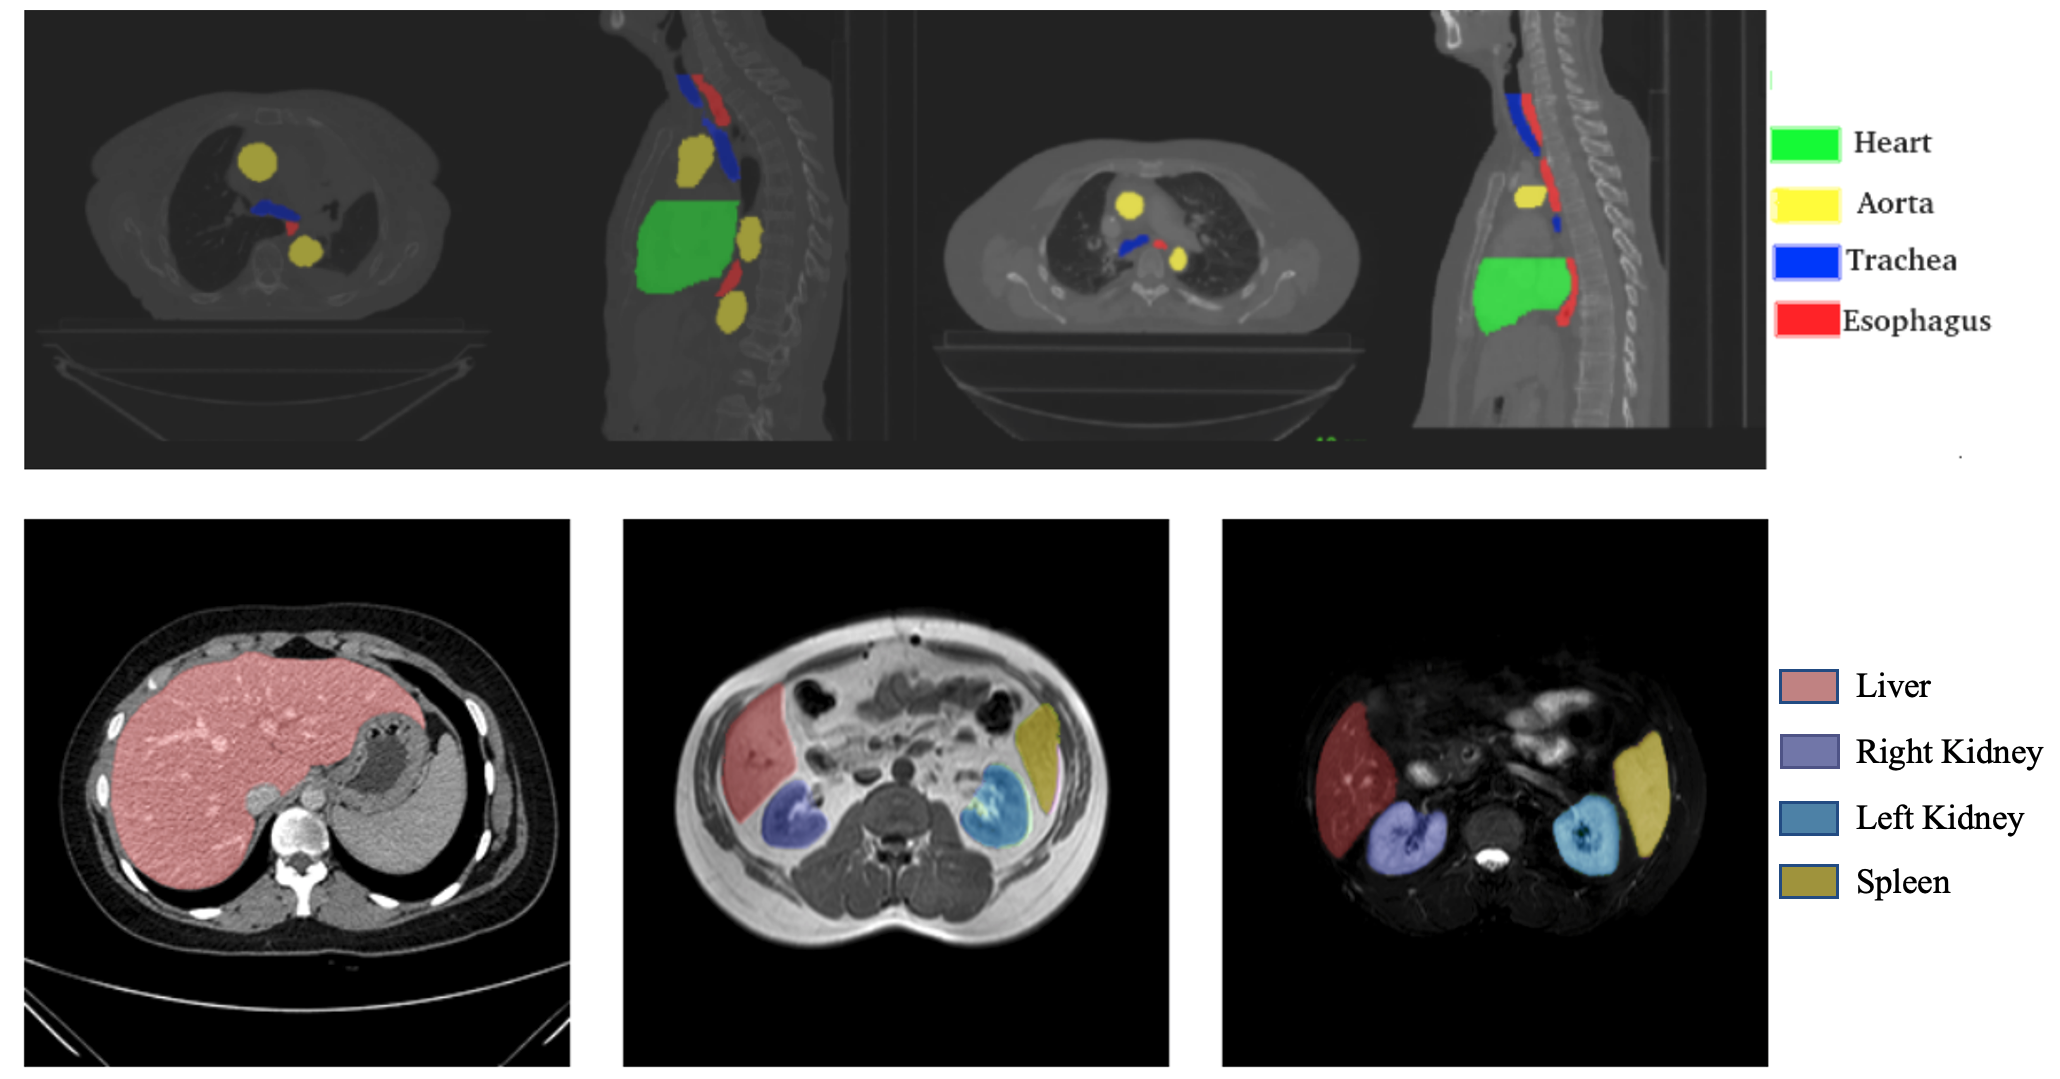
\includegraphics[width=1.0\textwidth]{img/c1/intro_1.png}
        \bicaption{医学图像中语义分割任务的例子:第一行是胸部 CT 图像\citep{lambert2020segthor},分割标注覆盖在原图像上,第二行是腹部的 CT、MR T1 和 MR T2 图像及其分割标注~\citep{kavur2021chaos}。}
        {Examples of medical image semantic segmentation. The first row shows images of thoracic organs, with an overlay of the manual segmentation, and the second row shows slices from abdominal organ in CT、MR T1 and MR T2 phases.
        DeepLab model training using image-level labels.}
        \label{c1_fig1}
    \end{figure*}


传统的图像语义分割根据图像的颜色空间、空间距离及纹理等特征进行处理,包括聚类分割\citep{coates2012learning}、阈值分割\citep{ying2005fast}、决策树分类\citep{shotton2008semantic}、图割分割\citep{vicente2008graph}等方法。
随着深度学习技术,特别是卷积神经网络(convolutional neural network, CNN)在计算机视觉的广泛应用,语义分割技术迎来了新的发展。深度神经网络可以从大量的标注数据中自动学习提取丰富的高阶语义特征,并基于提取出的特征进行推理,预测图像的像素级标签。以全卷积神经网络(fully convolutional network, FCN)为开端的一系列分割工作,极大提高了该任务的准确度与应用场景的广泛性。

训练基于深度学习的分割模型,通常需要一个较大的数据集,并且依赖大量像素级别的标注(能够准确地划分出物体边界)。然而,在医学领域,由于缺乏有经验的标注者和物体边界的视觉模糊性,获得这种高质量的标签往往是困难的。并且,像素级别的标注也是非常昂贵和耗时的。极高的标注成本提高了语义分割方法落地的难度,也限制了其应用范围的广度。因此,如何降低标注难度和成本是一个实践中非常关心的问题。
%% 划掉(两块的讲法是,我们研究弱监督的两种形式:1.不准确监督... 2. 不确切监督... )
%% 划掉(随后每一块里的开头都会定义好名字:语义分割的不准确监督、语义分割的不确切监督。行文中都可以用弱监督语义分割(因为假定提出的方法是可扩展的,解决弱监督分割的问题的))
% 整体来说,弱化两个分类名称,多用统一的“弱监督语义分割”表述
% 弱监督的两种形式:基于弱标签和基于噪声标签 (不引入额外的概念名词)

为了解决上述问题,我们探索语义分割的弱监督学习,具体地,研究弱监督的两种形式:基于弱标签和基于噪声标签的学习。
基于弱标签的弱监督语义分割\citep{papandreou2015weakly,rajchl2016deepcut,cai2018accurate,ji2019scribble,kervadec2020bounding},它放弃要求较高的全标注,采用弱标签方式,并探索对应的基于弱标签的高效的分割方法。基于噪声标签弱监督语义分割\citep{Zhu2019PickandLearnAQ,Xue2020CascadedRL,Zhang2020RobustMI},它研究基于噪声标签,探索具有处理噪声能力的鲁棒的分割方法。
这两个方向探索的目标都是,在有限条件的数据标注下,尽可能提高分割效果,以接近基于完整准确标注方法(即全监督语义分割)的上限。

% 基于弱标签:问题转化、目标与实际意义
基于弱标签的弱监督语义分割,采用一些简单形式的标注方式,比如边界框、涂鸦式标签、点标签等,来进行图像分割模型的学习。图~\ref{c1_fig2}列出其中几种标签的示例,各自对应着不同的标注成本。
    \begin{figure*}[tbp]
        \centering 
        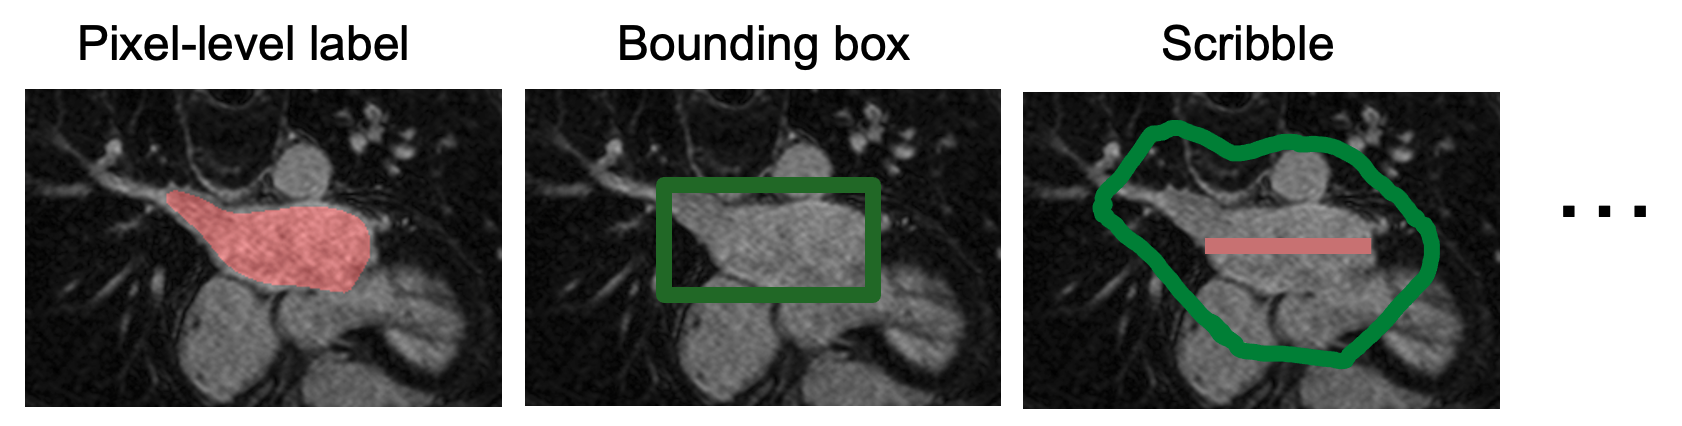
\includegraphics[width=1.0\textwidth]{img/c1/intro_2.png}
        \bicaption{医学图像上的弱标签示意图。从左到右依次是完整标签,边界框标签和涂鸦式标签。}
        {Different annotations on medical images. From left to right: groundtruth, bounding box and scribble.}
        \label{c1_fig2}
    \end{figure*}
由于弱标签提供的标签信息远少于全标注,语义信息有限,所以直接应用现有分割方法的输出精度较低。故而,如何充分利用弱标签来提高语义分割的效果,是一个研究热点。
在此方向的探索,实质上是采用各种技术来弥补数据不足带来的效果下降,一种较好的弱监督分割方法,能够广泛应用到各种数据不足的场景,解决实际中的数据难题,对扩大深度学习技术的应用场景有重大意义。

% 基于噪声标签的语义分割:问题定义、目标和实际意义
基于噪声标签的弱监督语义分割,是指训练数据中有一定比例的错误标签。由于医学图像本身的标注难度,分割标签噪声是难以避免的,图~\ref{c1_fig3}给出一些标签易出错区域的例子。
噪声标签会直接干扰神经网络的学习能力,降低模型的分割效果。这个任务中的核心问题是如何识别并处理噪声标签,减少其对神经网络的影响。现实中由于数据收集的复杂性,噪声标签是很常见的,探索这一问题,可以高效利用这些已有的噪声标签。
    \begin{figure*}[tbp]
        \centering 
        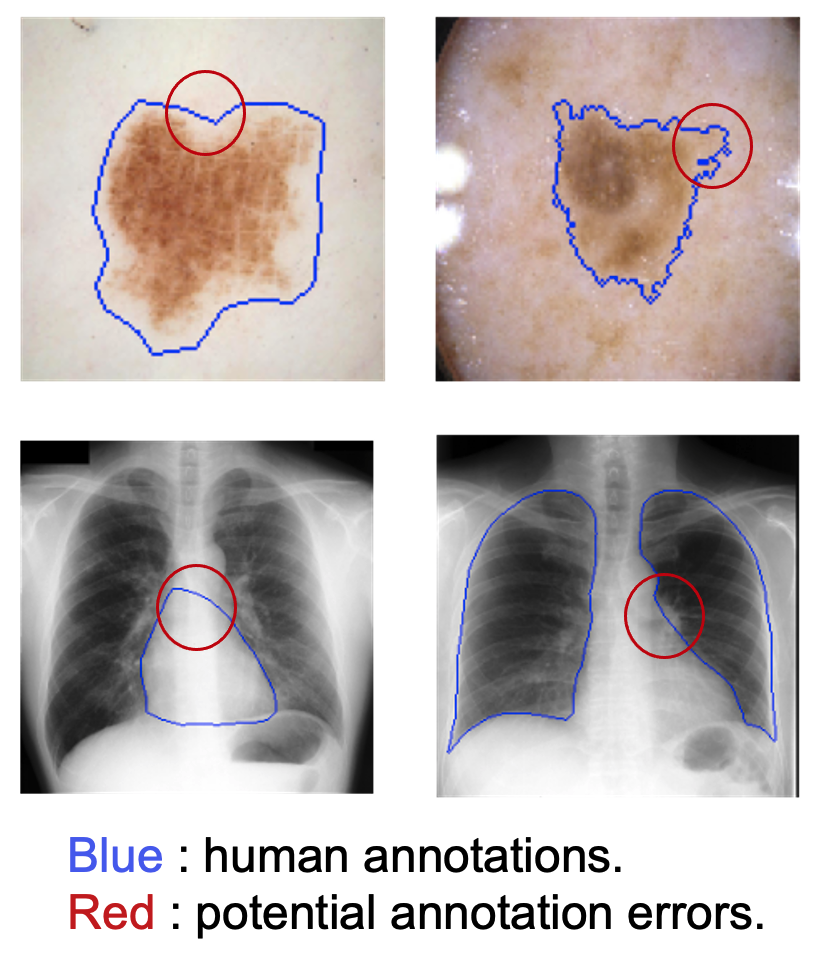
\includegraphics[width=0.7\textwidth]{img/c1/intro_3.png}
        \bicaption{医学图像标注的噪声标签示意图。蓝色区域为人工标签,红色区域是可能的标签错误。}
        {Examples of noisy annotations of medical images. Blue curves show human annotations, while red curves point to potential errors.}
        \label{c1_fig3}
    \end{figure*}

% 弱监督工作的局限,引入形状先验的意义
在基于弱标签的弱监督语义分割,本文研究的重点是结合形状先验的分割方法。仅仅依靠标注的粗标签,能获取的信息是有限的。本文希望在弱监督语义分割中引入形状先验,来弥补训练标签的不足。
只把分割工作视为每个像素的分类任务,会忽略其整体的几何结构。在分割任务中,局部视角下确实每个像素都只利用其特征做分类,但在全局视角下物体有整体的形状。这种整体结构的建模与利用,能够作为先验信息,克服局部视角的错误或缺失,引导模型产生更准确完整的预测结果。
在医学图像领域,大多数物体都具有相对固定的形状,一类物体也都具有一定程度的形状相似性。利用好形状先验,能够高效地解决弱标签带来的挑战,生成更加准确的分割结果。

% Noisy工作的局限,引入结构先验与空间关系的意义
在基于噪声标签的弱监督语义分割中,本文重新考虑训练中的基本样本单元,以利用分割任务中的像素间相关性和空间先验。
过去的许多工作,忽略了分割任务的特性,把每个像素看做独立同分布的样本来建模,这是不符合实际的。我们考虑使用更灵活的表示和训练策略,来捕捉分割中图像的底层特征与性质,从而更准确地利用和处理噪声标签。


\section{研究背景及意义}
% 医学图像语义分割 背景
在图像语义分割任务中,全监督学习技术已经取得了很多进展,达到了较高的精度。这是其后研究弱监督语义分割的基础。
\citet{long2015fully}~针对传统神经网络要求固定尺寸的图像输入的问题,首次提出了接受任意尺寸输入的FCN。FCN~用全卷积层替换~CNN~输出端的全连接层,实现端对端的稠密预测。在此基础上,DeepLab~为了更精细的分割效果,在 CNN 的输出后使用全连接的条件随机场,以优化定位精度。更进一步,\citet{ronneberger2015u}~提出了一种编码器-解码器结构 U-Net,这种结构被广泛应用在医学图像上。U-Net~的编码器采用一系列的卷积层和下采样操作,逐级提取语义信息,解码器则是一系列的卷积层和上采样操作,逐级恢复图像细节。U-Net兼顾了分割精度与效率。

除了~2D~医学图像,医学图像领域也有许多~3D~形式的分割任务。3D~U-Net 扩展了 U-Net,主要通过 3D 卷积单元替换 2D 卷积单元完成。这样整个 3D 图像可以直接输入进模型,输出端预测得到 3D 分割结果。V-Net 则通过把残差连接引入卷积模块,并且用卷积层代替上采样和下采样的池化层,并提出 Dice loss 来克服类别不均衡,提高 3D 分割网络的表达能力与精度。

\citet{isensee2019automated}~提出了 nnU-Net,这是目前提出的泛化性能最好的分割系统。它是一套鲁棒的自适应的框架,适用于大多数 2D 和 3D 图像,探索了自适应模型结构、前处理、训练和推理阶段的各种方案。

% 弱标注 related  背景
然而,全监督学习所需的标注成本很高,弱监督学习是降低标注成本的一种方法。近年来有很多工作对弱监督语义分割进行探索,并取得了相当地进展。
基于弱标签的弱监督分割,其基本问题是,采用什么形式的弱标签,继而如何仅仅利用弱标签,来训练需要大量数据的神经网络。
\citet{lin2016scribblesup} 提出使用涂鸦(scribble)进行图片标注,并且设计了一种算法,可以用涂鸦标注监督训练语义分割卷积网络。该工作先设计一个图模型,以把涂鸦标签传播到未标注像素上,同时,利用传播后的标签学习一个全卷积网络,并反过来提供语义信息给图模型。
\citet{papandreou2015weakly} 探索使用边界框(bounding box)或图像级标签的标注方法,并提出了一种弱监督下的期望最大化(expectation maximization, EM)算法来训练语义分割模型。这种算法迭代地进行弱标注约束下的未知像素标签估计,和使用估计得到的标签优化分割神经网络。EM 算法在后续的工作中被广泛使用。

% 弱标注的挑战
尽管这些工作在分割效果上取得很大提高,但未能探索分割任务中的形状先验、结构先验等约束,容易生成不准确的物体形状。物体并不仅仅有局部视角下的特征,也有整体的连续性与形状,充分考虑局部特征与整体特征的结合,对提高分割效果及算法的鲁棒性泛化性,具有重要意义。
\citet{tang2018regularized} 采用基于正则化损失的弱监督方法,通过设计具有底层分割特性的正则项,来隐式地实现分割网络对底层特征的关注。这种正则项损失采用了马尔可夫随机场和条件随机场的形式。
\citet{kervadec2020bounding} 探索在边界框的弱标注方法上,在模型中引入一些全局约束条件,包括框内的紧致性先验和框外的全背景先验。这些约束条件被转化融合进损失函数中进行优化。
由于这些工作对先验的表达不足,或者依赖于特定的标注形式与超参数,有一定局限性。在弱监督分割中结合物体形状先验,仍然是一个需要探索的方向。

% 有噪声标注 related
基于噪声标签的弱监督分割考虑另一种情况:标签中有一定比例的错误。错误标签如果不做处理,会直接损害神经网络的效果。近来一些工作借鉴分类任务的工作,对这一领域进行了探索。
\citet{Zhu2019PickandLearnAQ} 提出一种标签评估网络来自动评估标签质量,同时训练评估网络和分割网络,来自动重调整损失函数,以减轻错误标签对网络的负面影响。
\citet{Zhang2020RobustMI} 设计了一种三网络同步学习的框架,用任两个网络来选择有价值的样本给另一个网络,这种同步训练并相互学习的方式克服了单网络容易过拟合的缺点。
% 有噪声标注的挑战
然而,这些工作在利用正确标签的方法上仍有不足,忽略了分割区域中的特征关系与空间结构,并且对分割网络的学习方式不够鲁棒。在这些方面的探索,依旧存在挑战性。

\section{本文研究内容}
本文研究根据分割任务的特点,分别探讨引入形状先验在弱监督语义分割中的作用,和基于图像底层特征表示鲁棒学习方法。本节分别讨论基于弱标签和噪声标签的弱监督语义分割中现有的挑战与不足,根据我们的对比观察给出相应的思考。然后基于这些思考,我们提出了自己的解决方法。对基于弱标签的语义分割,我们用自学习的方法捕捉到物体的形状先验,以解决弱监督下分割形状的缺陷;对基于噪声标签的语义分割,我们利用超像素作为基本表示单元,并基于它进行模型更新和标签更新,以解决噪声标签的干扰问题。最后,我们总结了本文在这两个任务的主要贡献,并探索了形状先验、结构特征对于弱监督语义分割的重要性。

\subsection{基于弱标签的弱监督语义分割}
基于弱标签的弱监督分割任务,旨在探索基于弱标签的鲁棒的语义分割方法,以较少的标注成本达到较好的分割效果。本部分主要关注三维图像的语义分割,因为现实世界中,很多医学图像都是三维形态的(比如CT、MRI等),而很多工作已经探索过二维图像,却对三维图像探索得较少,我们尝试弥补这方面的不足。
在弱监督的三维图像语义分割领域,近来有很多工作采用把三维图像拆分成一系列二维图像的策略。然而,这些基于二维的方法,虽然取得了不错的效果,但应用在三维图像时有以下局限。首先,它们只是将生成的二维掩膜堆叠在一起作为最终输出,因此往往会产生不准确的物体形状\citep{kervadec2019constrained,2020bounding}。此外,他们忽略了分割物体在三维空间中的连续性,并且无法利用连续的二维切片之间的标签相关性。由于这些限制与不足,在给定足够的三维样本和较小的片间间距条件下(Baumgartner等人,2017),二维方法往往比三维方法的表现要差。更进一步,现有的多数弱标注形式并不高效,无法为学习医学图像中的物体形状先验提供较好的指引。

在本文中,我们提出了一种新的三维物体分割的弱监督学习策略,以解决上述的挑战。我们的主要想法包括两个方面。首先,我们提出了一种自学习方法,通过物体样本增强的方法,来捕捉目标物体类别的三维形状先验。随后,我们将这种学习到的形状先验纳入具有形状感知的分割网络的训练过程。另外,我们采用了一个稀疏的弱标注方案,以更好地利用物体掩膜的空间连续性,并在不增加整体标注成本的情况下促进形状上下文的学习。

为了实现这一目标,我们设计了一个由两个主要模块组成的深度神经网络:一个是标准的语义分割网络,它从三维输入图像中产生一个初始的三维分割掩膜;另一个是形状去噪网络,它对初始分割掩膜进行改进并输出一个最终的三维分割。为了训练深度网络,我们首先引入一种稀疏的弱标注方案,在该方案中,我们只标注三维数据的一个特定的二维图像切片的子集(可以将三维图像数据视作一系列连续的二维图像切片),同时对每张二维图像,我们设计了一种混合式弱标签,它结合了前景涂鸦和目标物体的一个宽松边界框。给定这样的弱标注形式,我们为前述的网络模型设计了一个迭代学习框架,交替进行像素级标签生成和网络参数更新。

具体地,我们首先使用弱标签训练语义分割模块,来初始化我们的网络模型,该模块为训练数据预测生成了初始分割掩膜。然后利用这些初始掩膜,我们用自学习方法来学习形状去噪模块。为此,我们选择具有最高置信度的掩膜预测作为目标形状,以此把形状去噪模块作为一个去噪自动编码器(denoising autoencoder)去训练\citep{vincent2010stacked,Sundermeyer_2018_ECCV}。为了模拟产生对应的有噪声的掩膜输入,我们根据初始掩膜预测中的经验错误模式,对目标形状应用了几种噪声增强方案。在模型初始化之后,我们的学习程序迭代地执行两步更新:像素级的伪标签生成,和神经网络学习。对于标签生成,我们采用一个不确定性过滤机制融合语义分割模块和形状去噪模块的预测输出,这使我们得以利用学习到的形状先验来提高标签质量。在网络学习中,我们冻结了形状去噪网络,并在原始弱标签和生成标签的双重监督下更新语义分割网络。

我们在三个公开的医学图像数据集上来评估我们的方法,这三个数据集的目标器官有各自不同的形状特征,分别是SegTHOR挑战赛\citep{trullo2019multiorgan}中的气管、2018心房分割挑战赛中的左心房和Promise12挑战赛\citep{Litjens2014EvaluationOP}中的前列腺。实验结果表明,我们的方法全都优于以前的方法。此外,我们可以仅用少量的标注(10\%的二维切片标注)取得了鲁棒准确的结果,而其他现有方法在这种情况下效果很差。

\subsection{基于噪声标签的弱监督语义分割}
基于弱标签的弱监督语义分割,要解决的中心问题是防止分割网络过拟合到噪声标签的模式上。本部分沿袭之前工作的设定,研究二维图像上的鲁棒学习方法。
%由于该方向刚起步,现有工作较少,本部分沿袭之前工作的设定,研究二维图像上的鲁棒学习方法。
目前已经有一些工作尝试解决用噪声标签来训练分割网络的问题,这些尝试大体上可以分为两类。第一类方法以图像为基本单位,把每个图像样本的标签都视为正确或者错误,然后在训练过程中迭代地选择或重加权图像样本\citep{Zhu2019PickandLearnAQ,Xue2020CascadedRL}。具体来说,\citet{Zhu2019PickandLearnAQ}通过同时训练一个标签评估网络和一个分割网络,隐式地对图像的损失函数进行重新加权,而\citet{Xue2020CascadedRL}通过将协同教学(Co-teaching~\cite{Han2018CoteachingRT})方案扩展到一个三网络学习框架,显式地选择图像子集进行训练。然而,这种图像级别的加权策略在严重的噪声设定下不鲁棒,因为它们无法充分利用每张图像中具有正确标签的像素。为了解决这一局限性,第二类训练方法将分割视为像素级分类任务~\citet{Zhang2020CharacterizingLE,Zhang2020RobustMI},在训练中,根据最近的鲁棒的分类器学习策略来进行像素级别的样本选择或标签改进,比如置信度学习技术(~\cite{Zhang2020CharacterizingLE})或三网络协同学习方法\citep{Zhang2020RobustMI}。尽管他们更好地利用了标签,但基于像素的方法忽略了图像分割中的像素相关性和空间先验关系,因此容易在目标物体边界周围产生噪声预测,影响分割效果。

在这个工作中,我们为图像语义分割提出了一种新的鲁棒的学习策略,目标是利用图像的结构先验和像素标签的相关性。为此,我们采用了图像的超像素表示,并设计了一个迭代学习方案,这个方案结合了分割网络的噪声感知训练过程和噪声标签改进过程,两者都由超像素引导。这种结合使我们能够更好地利用分割标签的结构约束来进行模型学习,从而有效地减轻噪声标签的影响。我们注意到,虽然超像素在最近的工作中也被采用\citep{li2019supervised},但他们只用来改进噪声标签,而忽略了训练期间噪声标签的影响。

具体来说,在每次迭代中,我们首先使用选择的具有较小损失值的超像素子集来同时训练一堆孪生网络,这遵循了多视图学习框架\citep{Han2018CoteachingRT,Wei2020CombatingNL}。正如在协同教学方法中一样,这种多视图学习策略通过利用孪生网络的预测来约束网络训练。我们将每个超像素作为一个数据样本进行选择,因此能够在网络训练中引入空间平滑性并提供更好的物体边界指引。为了避免过拟合到噪声标签,我们根据超像素的损失值统计,为联合学习设计了一个自动停止的标准。在网络训练之后,我们使用网络预测来估计超像素标签的置信度,并对置信度最低的标签子集进行修正。这种标签修正方法使我们能够在后续模型训练中提高标签质量,提升训练效果。网络和标签更新会互相迭代,直到标签修正无法再取得进一步的改善。

我们在两个公开的基准数据集上评估了提出的方法,即 ISIC 皮肤病变数据集\citep{Gutman2018SkinLA}和 JSRT 胸部 X 射线数据集\citep{Ginneken2006SegmentationOA,Shiraishi2000DevelopmentOA},并探索了大量的噪声水平设定。在一系列的噪音水平区间,实验结果表明,我们的方法持续超过以往的工作,并表现出优越的训练鲁棒性。

\subsection{主要贡献}
本文从降低分割任务中所需标注成本入手,分别在基于弱标签和噪声标签弱监督语义分割两方面做出了贡献。

在基于弱标签的弱监督语义分割任务中,我们的主要贡献有三个方面:
\begin{enumerate}
\item 我们设计了一种形状感知的弱监督三维图像分割方法,它将自学习得到的的形状去噪网络纳入分割框架。我们还设计了一种迭代方法来进行有效的神经网络学习。
\item 我们为三维图像分割提出了一种新的稀疏的混合式弱标注策略。
\item 在相同的标注成本下,我们的方法在多种标注密度的设定下实现了最好的性能。
\end{enumerate}


基于噪声标签的弱监督语义分割任务中,我们的贡献分以下三方面:
\begin{enumerate}
    \item 在基于噪声标签的语义分割中,我们引入了超像素表示,以通过利用图像结构先验来增强模型的鲁棒性。
    \item 我们设计了一种包括模型更新和标签改进的迭代学习策略,以充分利用训练数据并逐步提高分割质量。
    \item 与当前最好的方法相比,我们的方法在一系列噪声水平设定下,实现了更好的性能和鲁棒性。
\end{enumerate}

\section{本文结构}
本节介绍全文的行文组织结构。

第一章为绪论部分,主要介绍医学图像语义分割的标注挑战的背景,并引出基于弱标签和噪声标签的弱监督语义分割这两个任务,随后介绍本文在这两个方向的主要研究内容。

第二章为相关工作部分,我们对医学图像分割、弱监督语义分割、结合形状先验的学习、鲁棒学习等方向的现有工作进行梳理总结。

第三章开始详述第一个方向的内容,即结合形状先验的弱监督语义分割。本部分我们先形式化描述弱监督分割任务,然后引出我们设计的结合形状先验的分割模型。再后介绍我们提出的稀疏的弱标注策略、模型训练过程,最后是详尽的实验来验证模型的效果以及和其他方法在定性定量的对比。

第四章是第二个方向的内容,即基于噪声标签的语义分割。这部分与上一章结构相似,依次介绍了该任务的形式化描述,模型设计,超像素表示,迭代的模型学习方法,实验对比与分析等部分。

第五章是全文的总结与展望。该部分总结了我们在弱监督语义分割的两个方向的方法设计与贡献,并探讨了该领域未来的研究趋势。
\chapter{相关工作}
本文研究基于弱标签和噪声标签的弱监督语义分割,在基于弱标签的语义分割中,我们的研究重点是如何结合形状先验,在基于噪声标签的语义分割中,我们关注如何利用图像结构和标签关系。本章分别介绍基于弱标签和噪声标签的语义分割,在基于弱标签的分割学习中,为了在缺少完整训练数据的条件下学习形状先验,我们介绍了自学习方法和去噪自编码器的工作。

\section{基于弱标签的语义分割}

我们先在~\ref{sec:rel_wss}节介绍通常的基于弱标签的语义分割的相关工作,它们通过标签传播或先验约束取得了一些进展,但鲜有工作探索结合形状先验的方向。本文目标是设计方法从弱标签中自学习物体的形状先验,用于分割形状去噪。为了解决形状学习中训练数据缺乏的问题,我们在~\ref{sec:rel_stl}节总结了自学习方法;为了根据形状先验学习去噪能力,我们在~\ref{sec:rel_dae}节调研了降噪自编码器的相关工作。

\subsection{基于弱标签的分割学习} \label{sec:rel_wss}

为了降低标注成本,基于弱标签的语义分割采用粗粒度的标签,比如图像级标签(\cite{wang2020self,fan2020learning,chang2020weakly}),边界框(\cite{papandreou2015weakly,khoreva2017simple,song2019box})和涂鸦式标签(\cite{lin2016scribblesup,vernaza2017learning,tang2018regularized})。这些弱标签的标注成本远低于完整标签,研究该任务对提高数据标注的利用效率有重要意义。现有的方法大致可以分为两类,第一类采用迭代学习的框架,即先传播监督信息,生成伪标签,再用其训练模型。第二类方法应用基于正则项的端到端训练框架,避免了生成伪标签的过程。接下来我们对这些工作进行详细介绍。


\citet{papandreou2015weakly}探索了在边界框和图像级标签这样的训练数据的学习算法。该工作为弱监督的语义图像分割模型训练开发了期望最大化方法,来解决模型训练不足的问题。在标签标注成本上,收集图像中每个类别周围的边界框标注会比逐像素标注快大约15倍\citep{lin2014microsoft},而收集图像级标签的标注成本更少。该文作者提出的期望最大化方法,在估计(被弱标签约束的)像素标签和用随机梯度下降方法优化深度网络参数这两个阶段交替进行。

在图像级标签上,作者定义了该问题的概率图模型,并根据该模型,用期望最大化算法来从训练数据中学习模型参数,如图~\ref{c2_fig1}。考虑求期望阶段偏差(bias)的不同形式,作者提出了两种具体方法:EM-Fixed 和 EM-Adapt。在 EM-Fixed 中,根据图像级标签为每个像素设置固定的概率偏差,施加图像的前景区域约束。在 EM-Adapt 中,根据图像级标签设定前景区域面积的偏差,来对前景区域施加约束。

在边界框标签上,作者也探索了三种方法来训练分割模型:Bbox-Rect, Bbox-Seg 和 Bbox-EM-Fixed,如图~\ref{c2_fig2}。Bbox-Rect 采用了简单的标签赋值方法,在边界框内的像素全部设为目标类别的标签,在其外的则为背景标签。这种简单的方法会引入一些边界框内的假正类标签,为了解决这一问题,Bbox-Seg 被提出。具体做法是,在边界框内不再全部设为正类标签,而是选择一定比例的边界框中心区域设为正类标签,边界框外则全部设为负类标签,然后构建一个条件随机场来推理其他的标签。这两种利用边界框来估计分割图标签的方法,都可以看作前处理步骤,随后利用生成标签来训练分割网络。此外,作者还提出了 Bbox-EM-Fixed,目标是在训练中改进分割标签估计,这是 EM-Fixed 的一个变种,不同的是仅对边界框内的像素施加前景偏差。最后这篇文章在 PASCAL VOC 2012 图像分割基准的评价指标有较高提升,验证了这些方法的有效性。


    \begin{figure*}[tbp]
        \centering 
        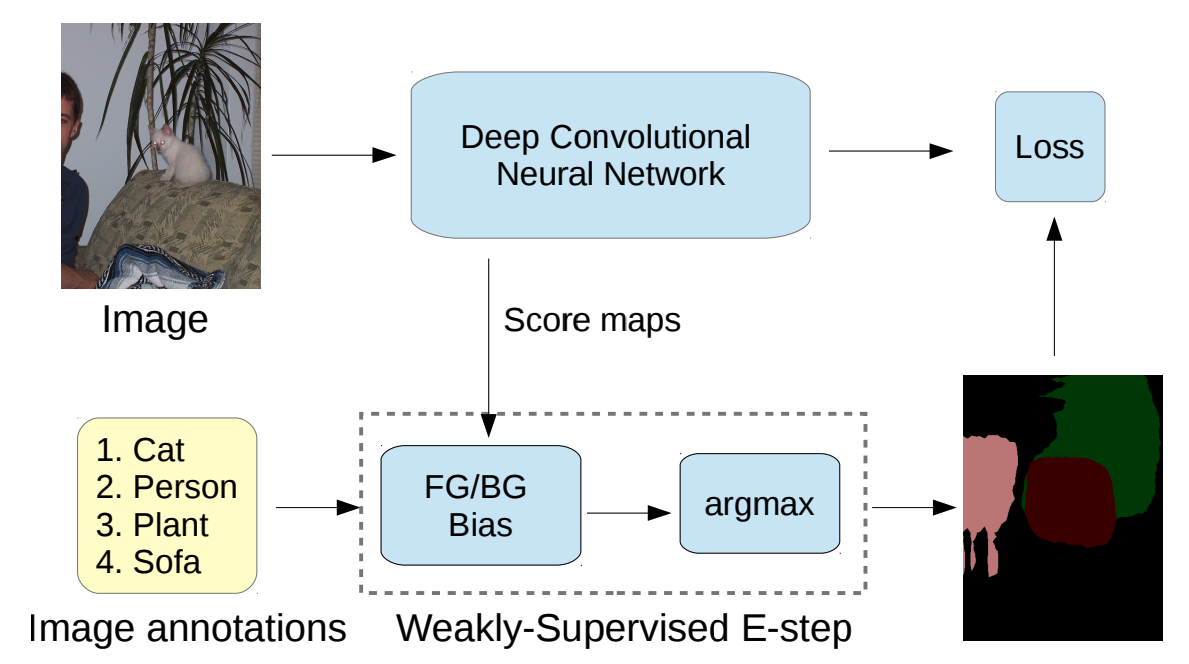
\includegraphics[width=1.0\textwidth]{img/c2/rel_a1.png}
        \bicaption{使用图像级标签的 DeepLab 模型训练过程。图自~\citet{papandreou2015weakly}。}{DeepLab model training using image-level labels. Figure is from~\citet{papandreou2015weakly}.}
        \label{c2_fig1}
    \end{figure*}

    \begin{figure*}[tbp]
        \centering 
        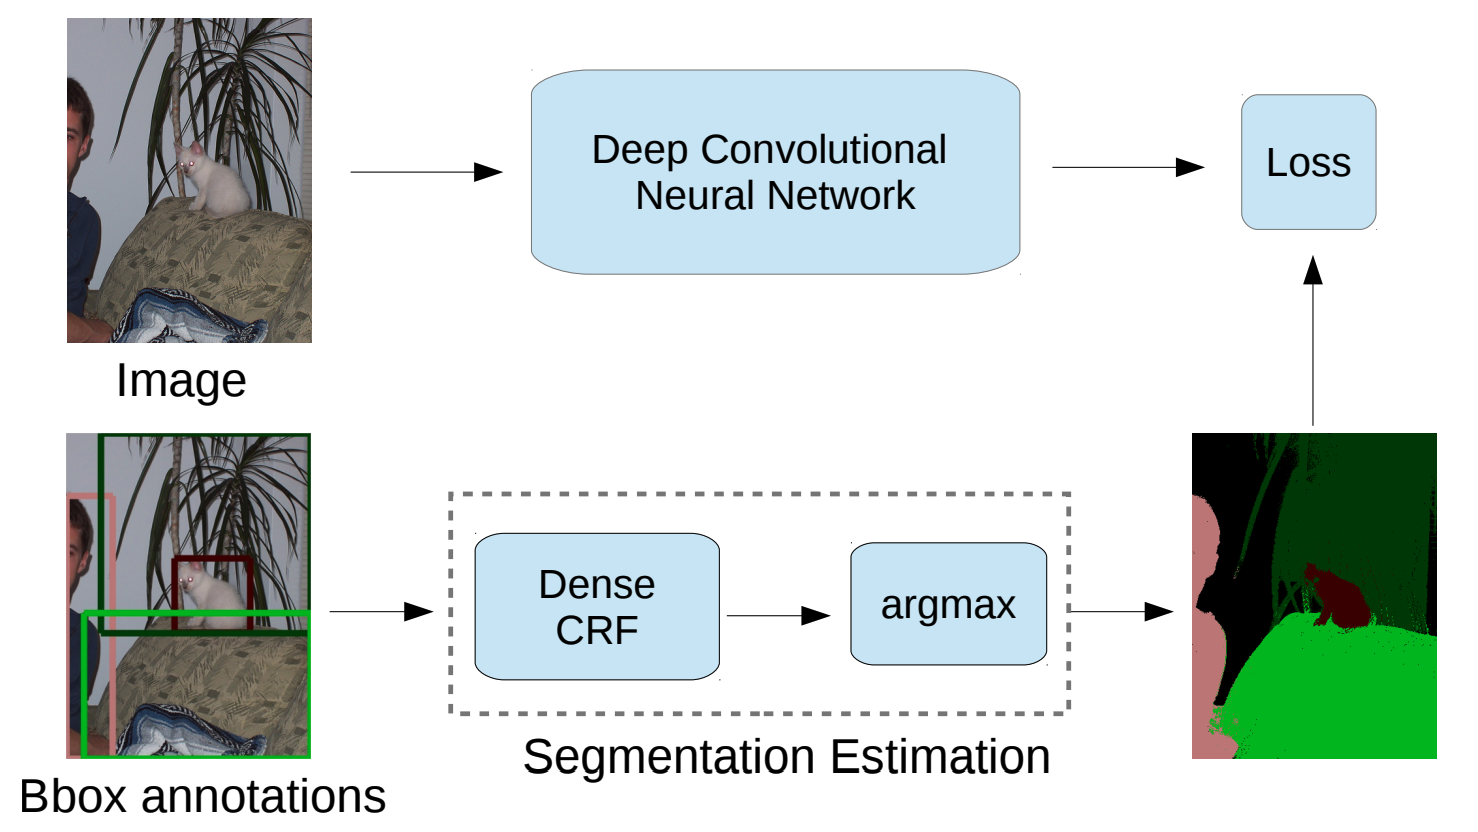
\includegraphics[width=1.0\textwidth]{img/c2/rel_a2.png}
        \bicaption{使用边界框标签的 DeepLab 模型训练过程。图自~\citet{papandreou2015weakly}。}{DeepLab model training from bounding boxes. Figure is from~\citet{papandreou2015weakly}.}
        \label{c2_fig2}
    \end{figure*}

    \begin{figure*}[tbp]
        \centering 
        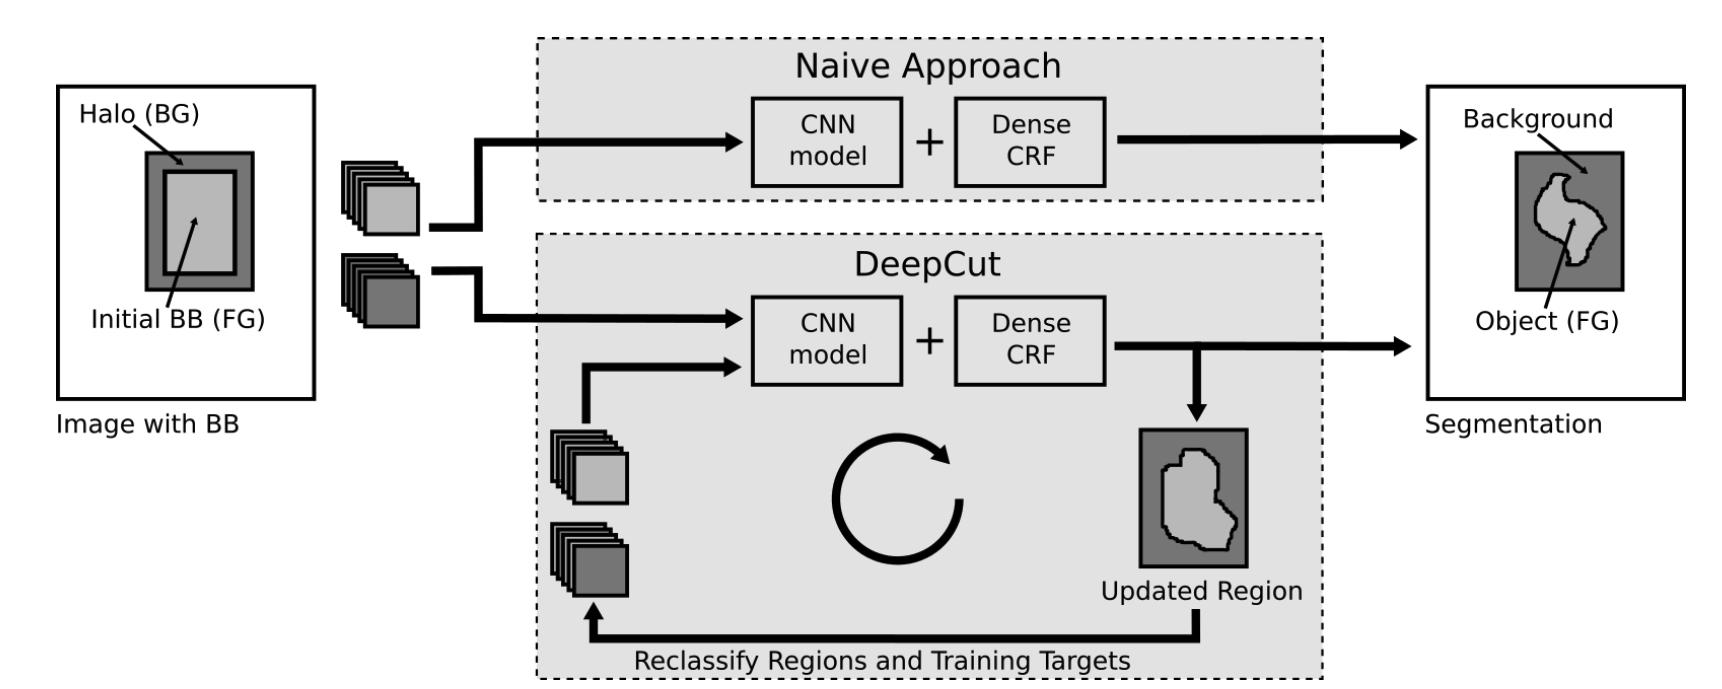
\includegraphics[width=1.0\textwidth]{img/c2/rel_a3.png}
        \bicaption{普通的 CNN 学习与提出的 DeepCut 方法的对比,后者迭代地更新学习目标。图自~\citet{rajchl2016deepcut}。}{Naive CNN learning versus the proposed DeepCut approach, iteratively updating the learning target classes for input patches. Figure is from~\citet{rajchl2016deepcut}.}
        \label{c2_fig3}
    \end{figure*}

    \begin{figure*}[tbp]
        \centering 
        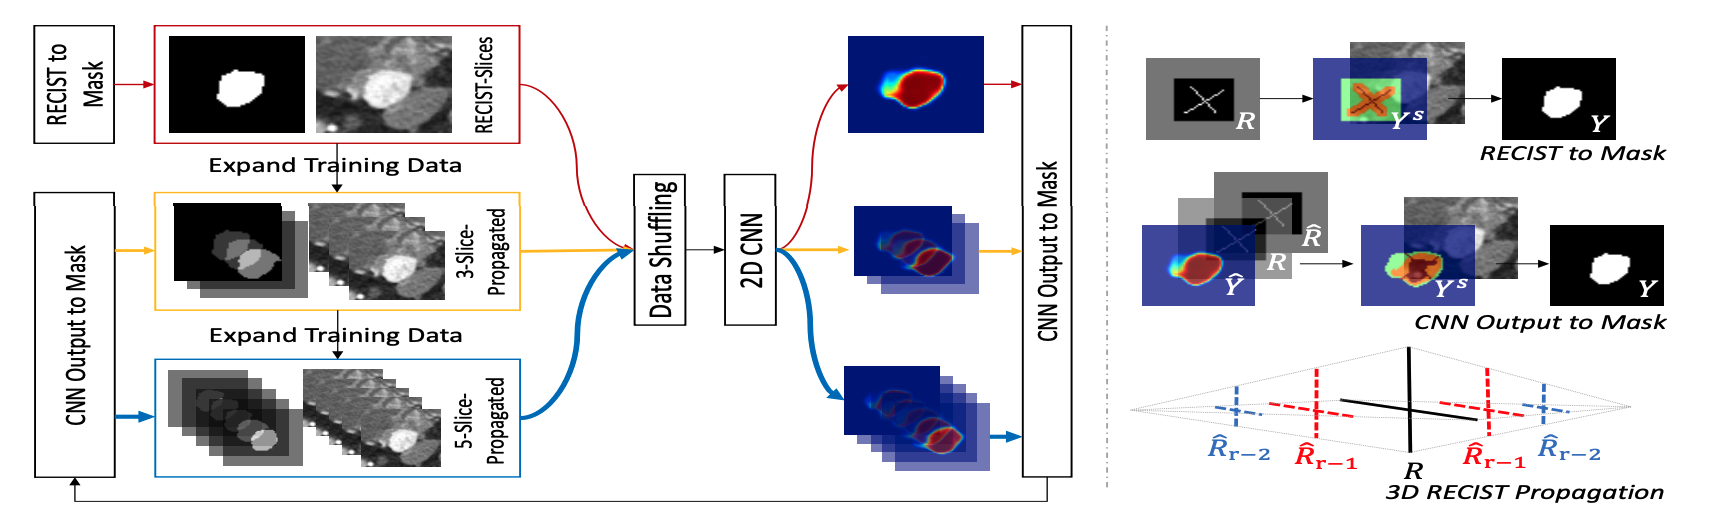
\includegraphics[width=1.0\textwidth]{img/c2/rel_a4.png}
        \bicaption{逐切片扩张的三维图像分割网络。图自~\citet{cai2018accurate}。}{The overview of slice-propagated 3D image segmentation network. Figure is from~\citet{cai2018accurate}.}
        % 左侧图展示了训练图像的增加过程,每次邻近的图片连通生成的弱标签一起加入训练。右侧图展示了弱标签的传播过程,RECIST 标签通过 GrabCut 传播,未标注图像通过分割网络的预测传播得到标签。
        % Left: Each time adjacent slices are fed into the training process. Right: RECIST labels are initialized by GrabCut method, and CNN outputs are used to gradually generate extra training data for lesion segmentation.
        \label{c2_fig4}
    \end{figure*}


    \begin{figure*}[tbp]
        \centering 
        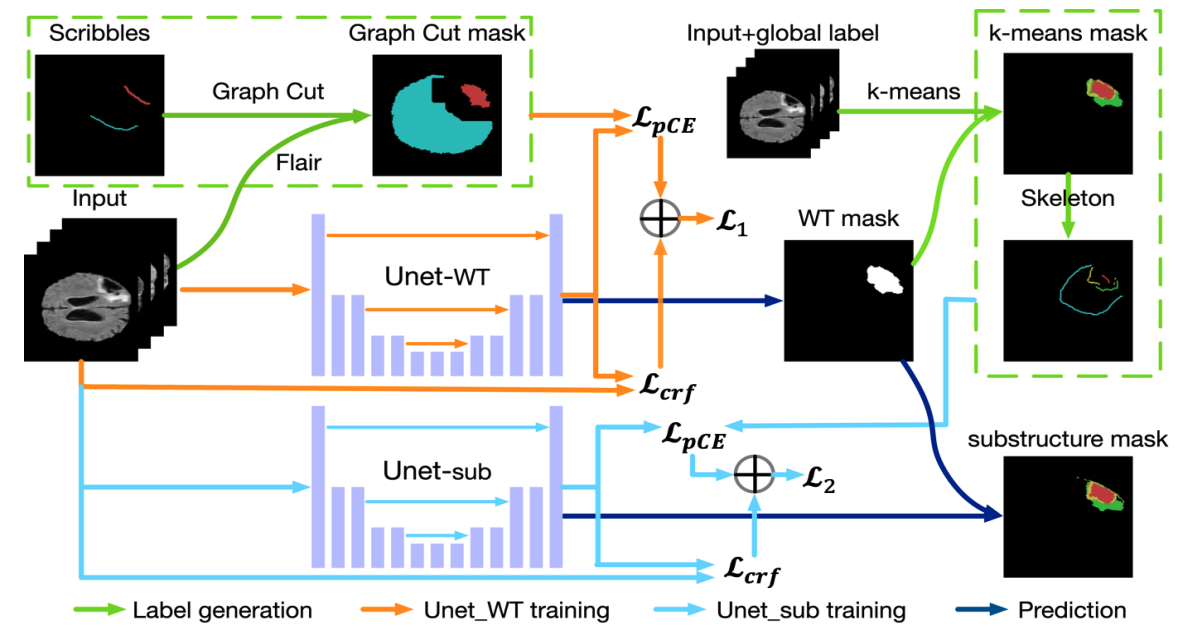
\includegraphics[width=1.0\textwidth]{img/c2/rel_a5.png}
        \bicaption{级联训练分割网络。图自~\citet{ji2019scribble}。}{Workflow of the proposed cascaded method. Figure is from~\citet{ji2019scribble}.}
        \label{c2_fig5}
    \end{figure*}


在 Deepcut\citep{rajchl2016deepcut}中进一步探讨了迭代地更新训练目标标签和模型参数的思想。该文的研究重点在边界框标签上。作者首先指出了边界框标签相对其他形式(比如涂鸦式)的优势,即对问题的空间约束(目标物体是完全包含在边界框内的),快速标注和轻量级存储(只需要定义对角线的两个端点)。本文目标是把神经网络模型和迭代的图优化方法相结合,以从粗粒度的边界框标签恢复像素级物体分割。受 GrabCut 方法的启发,其用一个基于像素强度的图模型迭代地拟合图像区域,随后被正则化以得到分割。该文将此任务定义为稠密连接的条件随机场下的能量最小化问题,提出迭代地更新训练目标,并且应用全连接条件随机场来规范分割。

模型结构如图~\ref{c2_fig3},作者对比了普通的 CNN 训练方法和提出的 Deepcut 迭代方法。重要的区别在于,Deepcut 对训练目标的迭代更新,可以渐进地提高模型训练的效果,这种迭代提高的方法要优于单一不变的训练目标。具体实现上,论文中还提出了DeepCut方法的变体,并与其它算法在弱监督任务进行了比较。Deepcut 方法在 Fetal Magnetric Resonance Dataset\citep{damodaram2012foetal}的这两个分割任务上取得了不错的精度,超过了之前的方法。

很多医学图像数据都是三维形态的,相比于二维图像,其标注成本大幅提高,因此基于弱标签的分割方法更为重要。三维图像可以直接处理,也可以分解为一系列连续的二维医学图像进行处理。
在三维图像上,\citet{cai2018accurate}研究利用现有的 RECIST直径 标签来生成完整的三维图像分割结果。三维图像的 RECIST 标签只在中心一张二维切片上(RECIST 标签是在中心切片的物体内部画出一对相互垂直的长轴与短轴),这篇文章要解决两个主要挑战,一是有弱标注图像的标签传播,以训练有效的分割网络,二是从已标注图像到未标注图像的标签传播,来分割出完整的三维物体。对前一个问题,作者采用无监督方法来初始化标签,对后一个问题,则利用分割网络的预测结果,来自动生成可信的标签。作者用一个迭代扩张训练图像的过程,来覆盖整个待分割的三维图像。总的来说,这篇文章把三维图像分割分解成一系列二维图像分割任务,通过标签传播和分割模型的分阶段训练来生成分割结果,最后堆叠组合为三维分割。

分割过程如图~\ref{c2_fig4}所示,是一个基于卷积神经网络的逐切片传播的分割方法。首先,为有 RECIST 标注的切片初始化分割标签,然后用这些切片训练分割模型。其后,利用初步训练的模型给临近的未标注切片初始化分割标签,用扩张后的切片及标签继续训练模型。这个过程不断迭代,直至所有切片都加入训练。作者在淋巴结数据集\citep{roth2014new}和 DeepLesion 数据集\citep{yan2018deep}进行实验,表明了所提出方法的优良性能。

另外,有些组织由多个子区域构成,比如脑肿瘤可能包括两到三种子区域,每个子区域都需要单独分割。如果每个子区域进行完整标注,耗时而低效。\citet{ji2019scribble}为这种任务提出了一种结合两种弱标签形式的标注方法,来减少标注成本。这种混合标注策略是,对整体的肿瘤区域用涂鸦式标签,而对各个子区域给出全局图像级标签。这种方式下,整体的肿瘤区域通过涂鸦式标签来学习,图像级标签用来引导子区域的聚类。这篇文章提出通过级联模型的方式,来解决这样具有层次结构的分割任务。

模型如图~\ref{c2_fig5}。受之前的级联网络的启发,这个模型采用先训练整体肿瘤分割,再子区域分割的方式。具体地,作者先用涂鸦式标签和由其初始化得到的图割标签,来训练整体肿瘤的分割网络。之后再在图像级标签的引导下,用无监督聚类方法提取肿瘤的各个子区域。最后把聚类得到的标签作为弱标签,来训练第二个子区域分割网络。作者还在分割网络训练中加入了 Dense CRF Loss,来提高分割边缘的连续性与准确性。这种方法在 BraTS2017 数据集\citep{menze2014multimodal}上进行了评估,在整体肿瘤分割和子区域分割上都取得了接近全监督上限的结果。

以上方法有共同之处:都是利用推理方法(GrabCut、CRF或初始化模型推理)来显式地生成伪标签,然后经处理后作为训练目标来优化模型。除了显式生成伪标签再训练,另一类方法直接使用弱标签训练,通过施加先验正则项来约束训练,以求较好的训练结果。\citet{kervadec2020bounding}和 \citet{tang2018regularized}是近期的重要工作。

\citet{kervadec2020bounding} 采用边界框标签,提出了一种基于全局约束的弱监督分割方法。作者首先提出了边界框的拓扑先验,包括框内的紧致性先验、框外的全背景先验和前景区域尺寸先验,这些先验被作为约束条件加入模型的训练目标。不过这些先验是不等式形式的约束,为了直接训练,作者通过对数障碍惩罚函数把不等式约束处理为损失函数的形式。这种利用全局约束来解决弱监督问题的方法,充分利用了领域先验知识,避免了只有少量标签训练的结果不确定性。并且基于约束方法能实现端到端的训练,可以避免显式生成伪标签过程中的错误传播。
    \begin{figure*}[tbp]
        \centering 
        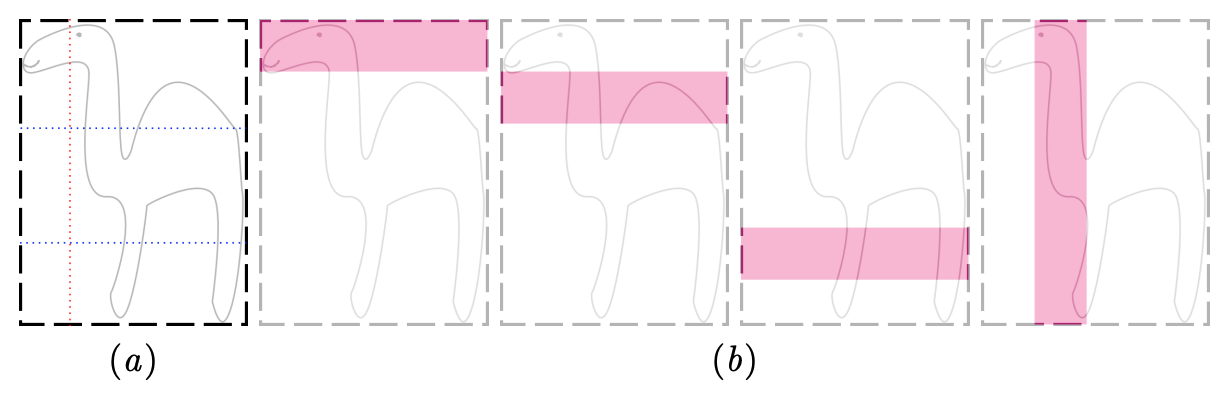
\includegraphics[width=1.0\textwidth]{img/c2/rel_a6.png}
        \bicaption{边界框标签的紧致性先验示意图:(a) 任一条竖直或水平的线段至少与一个前景像素相交。 (b) 更广泛地,宽度为 w 的线段至少与 w 个前景像素相交。图自~\citet{kervadec2020bounding}。}{Illustration of the tightness prior: (a) any vertical (red) or horizontal (blue) line will cross at least one pixel of the camel. (b) This can be generalized, where segments of width w cross at least w pixels of camel. Figure is from~\citet{kervadec2020bounding}.}
        \label{c2_fig6}
    \end{figure*}
全局约束充分考虑利用弱标签的信息。紧致性先验如图~\ref{c2_fig6}所示,基于边界框紧致地包围着目标物体边界,在框内的任意一条水平或竖直线段都会至少与一个前景像素相交。这种先验约束,能够防止训练过程中过拟合到背景类别而前景预测失败的问题。全背景先验是指边界框外的区域都属于背景类别,约束了前景的空间区域。前景区域尺寸先验,则是指目标物体在框内的面积比例有先验的下界与上界,利用尺寸先验可以约束分割结果的区域比例关系。这些全局先验通过对数障碍惩罚函数转换为标准的损失函数形式,可以直接使用随机梯度下降方法进行优化。
这篇文章在两个不同的公开数据集 PROMISE12\citep{Litjens2014EvaluationOP}和 ATLAS\citep{Liew2018ALO}进行试验,结果表明,这种方法可以接近全监督的分割效果,并且显著超过之前的 DeepCut 方法,同时避免了显式生成伪标签的耗时计算。

\citet{tang2018regularized}则在涂鸦式标签上探索把正则项融入损失函数,以实现在训练中结合浅层分割的效果(如图割法或 Dense CRF)。这篇文章通过设计 MRF/CRF 形式的约束项,来为分割模型引入浅层分割的特性如连续性、相关性、空间关系等。这种隐式的约束方法简化了弱监督的训练,避免了额外的 MRF/CRF 推理步骤来生成伪标签,提高了训练的质量和效率。这篇文章提出了几种用于弱监督的正则损失,分别是基于 Potts、Dense CRF 和 Kernelcut 的正则。作者通过 PASCAL VOC12\citep{pascal-voc-2012} 的实验对比了之前的生成伪标签的方法和不同正则损失函数,验证了所提出方法在弱监督语义分割的接近全监督的效果。


\subsection{自学习方法} \label{sec:rel_stl}
学习任务中,训练数据的缺乏是很常见的困难,而自学习方法可以作为一种解决方案。
自学习方法一般使用未标注的数据集进行训练,不同于自监督的学习方法中使用自身信号作为训练目标,自学习方法使用与目标任务一致的训练目标。因此,训练数据及标签产生、学习方法是其中考虑的重要方面。近期的工作将自学习方法应用于分类任务\citep{raina2007self,wang2013robust,feng2020autoencoder}、聚类任务\citep{li2017self,dai2008self}和定位任务\citep{bazzani2016self,jie2017deep},较好地利用了未标注数据进行训练,并随之提高目标任务的性能。我们考虑将自学习方法引入到弱监督语义分割中,解决形状先验的学习问题。就我们所知,迄今还没有工作探索过类似的方向。本节详细介绍一些运用自学习方法的相关工作。

在分类任务上,\citet{raina2007self} 通过在未标注数据集上应用自学习方法,利用学到的特征表示来提升在给定数据集的分类性能。自学习方法所使用的未标注数据集不受目标任务的限制。这篇文章出于对图像相似的基本视觉模式(如边缘模式)的观察,尝试从未标注数据中学习到简洁的、高阶特征的表示,这种表示可以使目标分类任务更容易。
具体地,作者所提出的自学习方法包括两个阶段。首先,在未标注数据上定义用稀疏编码构建高阶特征的优化问题,通过解这样的优化问题,可以得到图像的稀疏高阶表示。图~\ref{c2_fig7}展示了从图像块学习到的稀疏编码基向量,每个方格表示一种基。然后,这种已被学到的表征可以被应用于不同的分类任务,提高目标任务的效果。
    \begin{figure*}[tbp]
        \centering 
        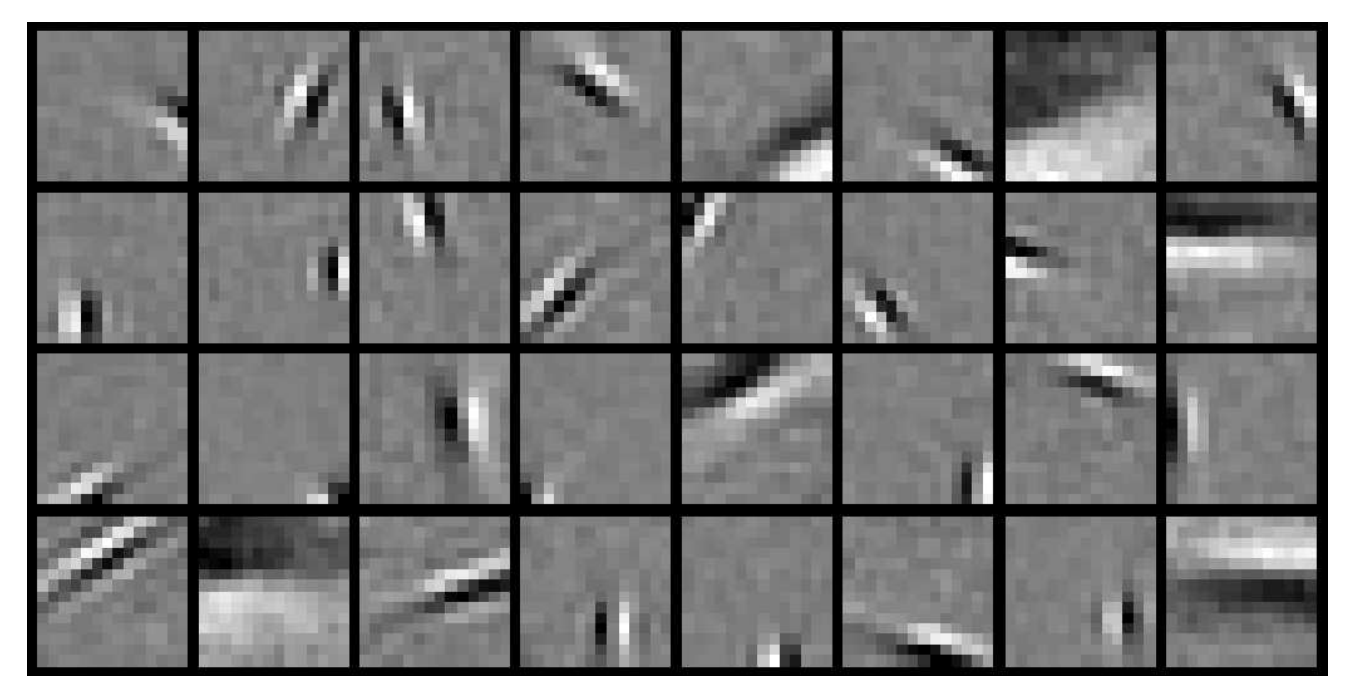
\includegraphics[width=1.0\textwidth]{img/c2/rel_b1.png}
        \bicaption{从图像块学习到的稀疏编码基向量的例子。图自~\citet{raina2007self}。}{Example sparse coding bases learned from image patches. Figure is from~\citet{raina2007self}.}
        \label{c2_fig7}
    \end{figure*}


在聚类任务上,\citet{li2017self} 观察到之前的自学习方法通常会忽略数据中的结构信息,因此专注于建立一个自学习编码框架,它可以有效地利用从辅助数据集抽象出来的丰富的低级模式信息,来描述目标数据集的高级结构信息。通过利用从辅助域和目标域中学习到的高质量字典,该方法为目标域中的样本学习了特征丰富的编码。由于许多类型的视觉数据已被证明包含子空间结构,作者在编码目标中引入了低秩约束,以更好地描述给定目标集的结构。这种提出的自学习的低秩编码框架,被形式化为一个非凸的秩最小化和字典学习问题。

模型框架如图~\ref{c2_fig8}。目标域的一个小数据集不足以提取有效的特征,通过利用辅助域的数据集,模型学习到一个共享字典,并对目标域的系数矩阵施加低秩约束,产生新的特征表示。随后这种特征表示作为图像聚类或分类任务的输入,提升训练性能。
    \begin{figure*}[tbp]
        \centering 
        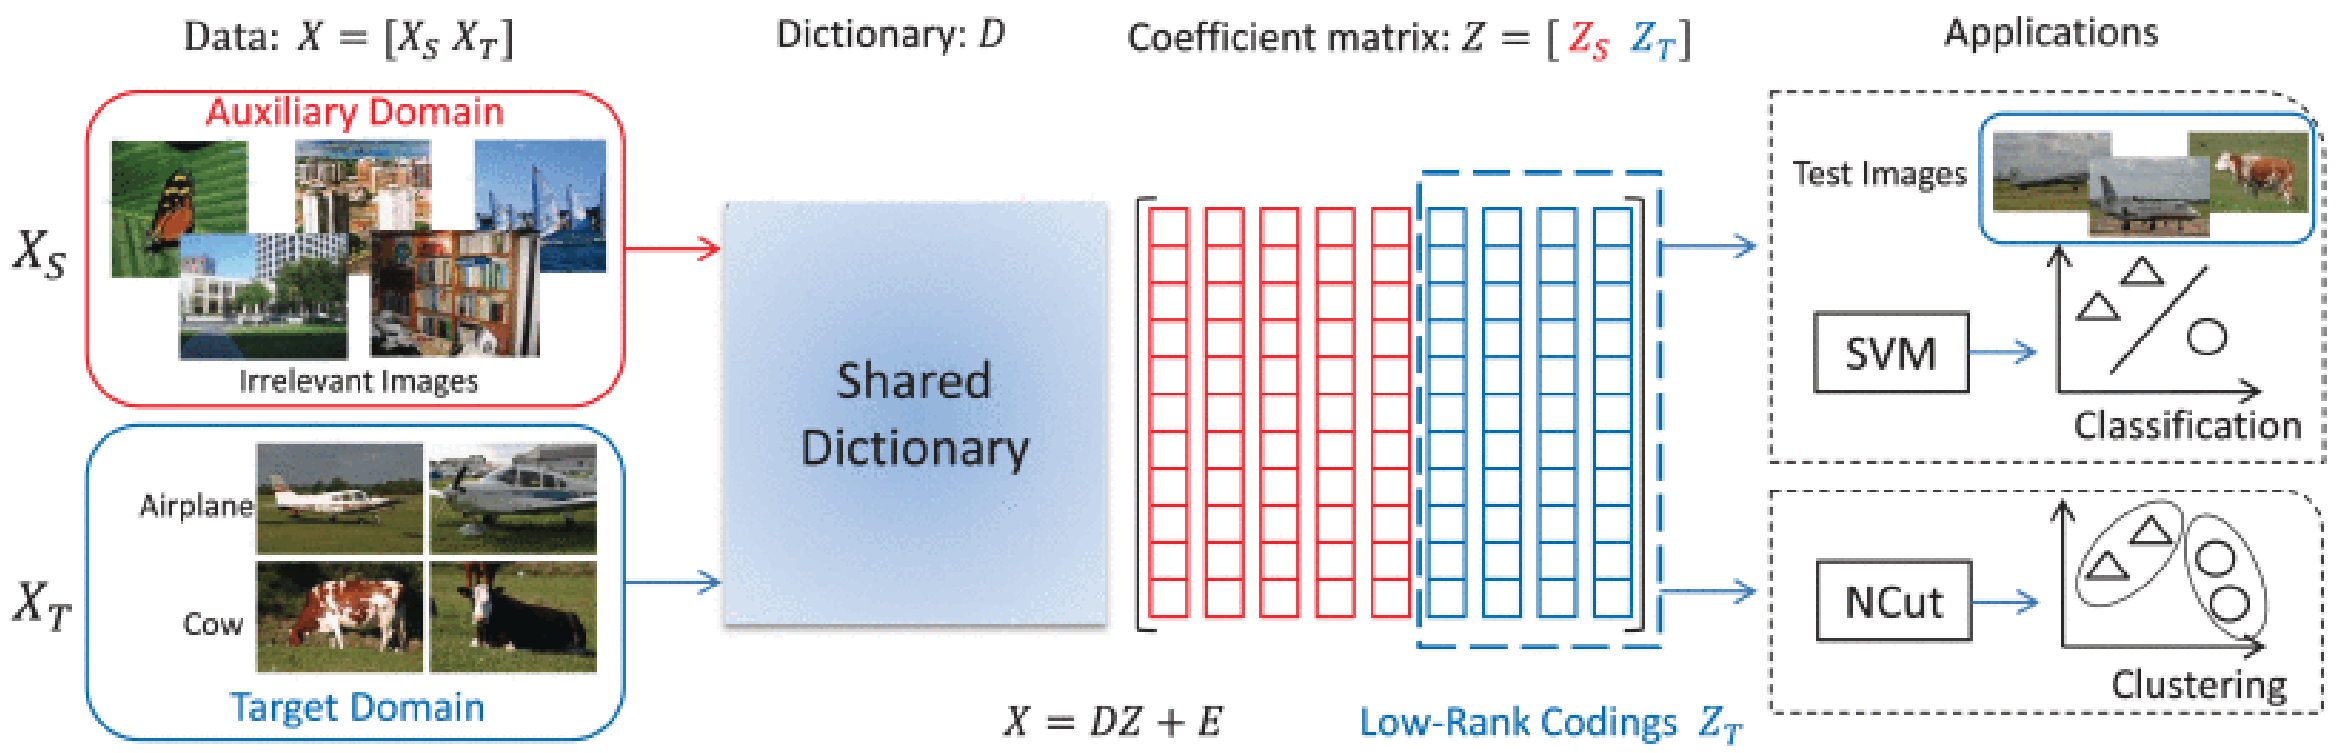
\includegraphics[width=1.0\textwidth]{img/c2/rel_b2.png}
        \bicaption{自学习的低秩编码模型。图自~\citet{li2017self}。}{Diagram of the S-Low coding framework. Figure is from~\citet{li2017self}.}
        \label{c2_fig8}
    \end{figure*}

在定位任务上,\citet{bazzani2016self} 设计了自学习的物体定位方法,不需要求真实的的边界框标签。其关键思想是,当人为遮挡图像的不同区域时输出的类别识别概率会变化,分析这种变化可以找到包含该物体的区域。图~\ref{c2_fig9} 描述了部分遮蔽出的图像在卷积网络的传播,从而影响识别概率的过程。
这种思想被融入到分层聚类方法,产生自学习的边界框标签。
    \begin{figure*}[tbp]
        \centering 
        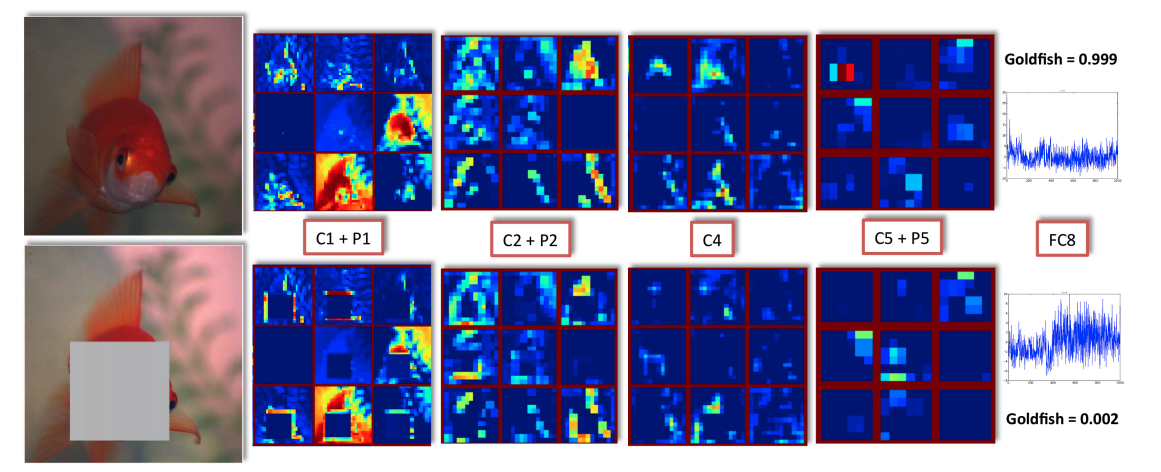
\includegraphics[width=1.0\textwidth]{img/c2/rel_b3.png}
        \bicaption{原图像(第一行)、被遮挡的图像(第二行)以及它们在卷积网络的各层输出。图自~\citet{bazzani2016self}。}{The image (first row), its mask-out version (second row) and the outputs of different layers of the convolutional network. Figure is from~\citet{bazzani2016self}.}
        \label{c2_fig9}
    \end{figure*}
这篇文章提出的物体定位方法在准确率和召回率上都优于之前的方法,在 ILSVRC-2012 数据集\citep{russakovsky2015imagenet}上比之前最好的方法有大幅的提升。并且,自学习方法生成的标签用于训练定位模型,定位结果与真实标注的训练结果非常接近。

\subsection{去噪自编码器} \label{sec:rel_dae}
去噪自编码器目标是将输入图像编码到高维空间的一个隐向量,该向量对噪声具有不变性,作为原始图像的鲁棒表示。近来有一些工作应用去噪自编码器来产生更好的图像表征和对输入的抗干扰能力。
\citet{vincent2010stacked} 探索构建一种基于堆叠的去噪自编码器的深度网络,来提高模型的泛化性与分类准确率。这些自编码器经过训练,具有对被噪声干扰的输入图像进行去噪的能力。这种网络表现出明显的低分类误差,这种以无监督方式学习的高层次语义表征也有助于提高后续 SVM 的性能。
具体地,图~\ref{c2_fig10}是去噪自编码器的结构。原始输入样本被随机地做噪声增强,然后通过自动编码器映射到隐向量,再通过自动解码器重建输入样本,重建损失函数由重建样本与原始样本的误差衡量。这种训练方式使模型具有了去噪和恢复原始干净样本的能力。这项工作表明了无监督任务目标中,去噪目标对学习一个有用的高阶表征的指导意义。
    \begin{figure*}[tbp]
        \centering 
        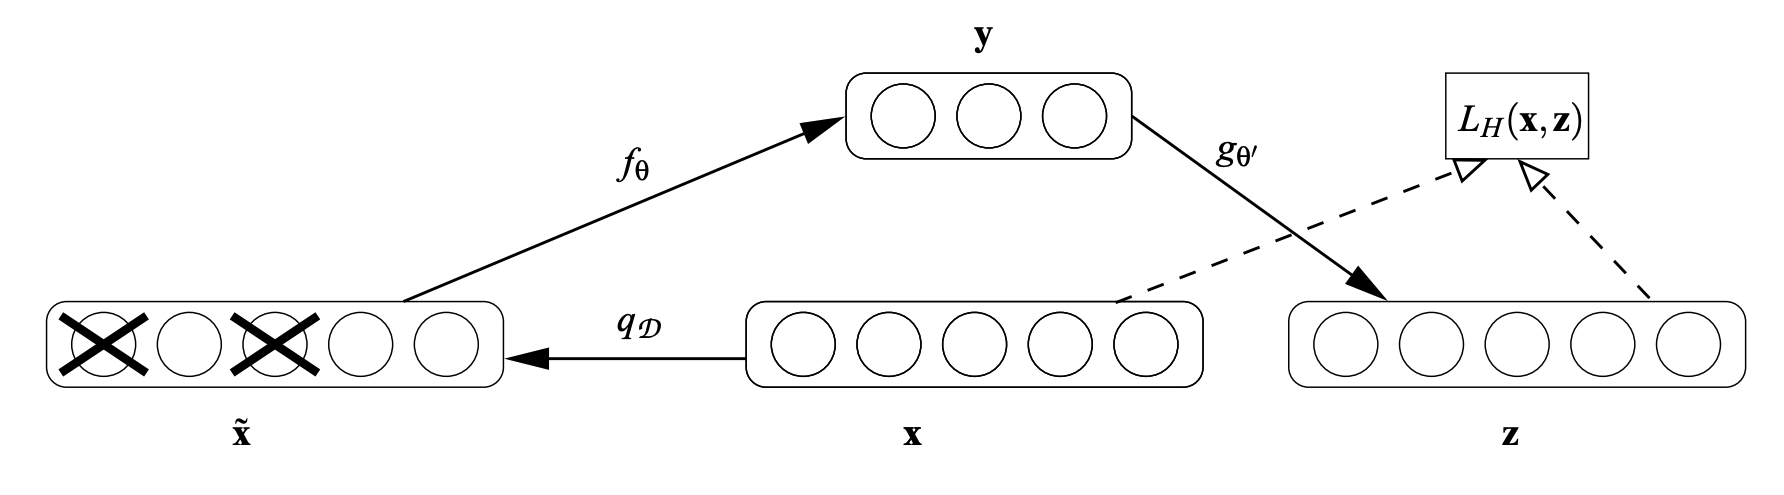
\includegraphics[width=1.0\textwidth]{img/c2/rel_b4.png}
        \bicaption{去噪自编码器的结构。图自~\citet{vincent2010stacked}。}{The denoising autoencoder architecture. Figure is from~\citet{vincent2010stacked}.}
        \label{c2_fig10}
    \end{figure*}

在三维姿态估计中,为了解决之前工作中对物体遮挡等动态变化、训练数据不足等挑战,\citet{Sundermeyer_2018_ECCV} 提出一种全新的基于增强型去噪自编码器的三维方向估计模型,并在使用域随机化的三维模型的增强视图上训练。增强型自编码器如图~\ref{c2_fig11},原始输入图像首先通过数据增强,产生几何结构和颜色增强后的图像,作为自动编码器的输入,输出的目标是回复原始输入图像。这种增强型自动编码器可以使模型具备动态环境下恢复准确姿态的能力,优点是:不需要真实的有姿态标签的数据,可以通用于多重测试传感器;不需要学习从输入图像到物体姿态的显式映射,而是采用样本隐空间的姿态隐式表示。基于此的姿态估计在 T-LESS 数据集~\citep{hodan2017t}和 LineMOD 数据集~\citep{hinterstoisser2011multimodal}都取得了先进的性能。
    \begin{figure*}[tbp]
        \centering 
        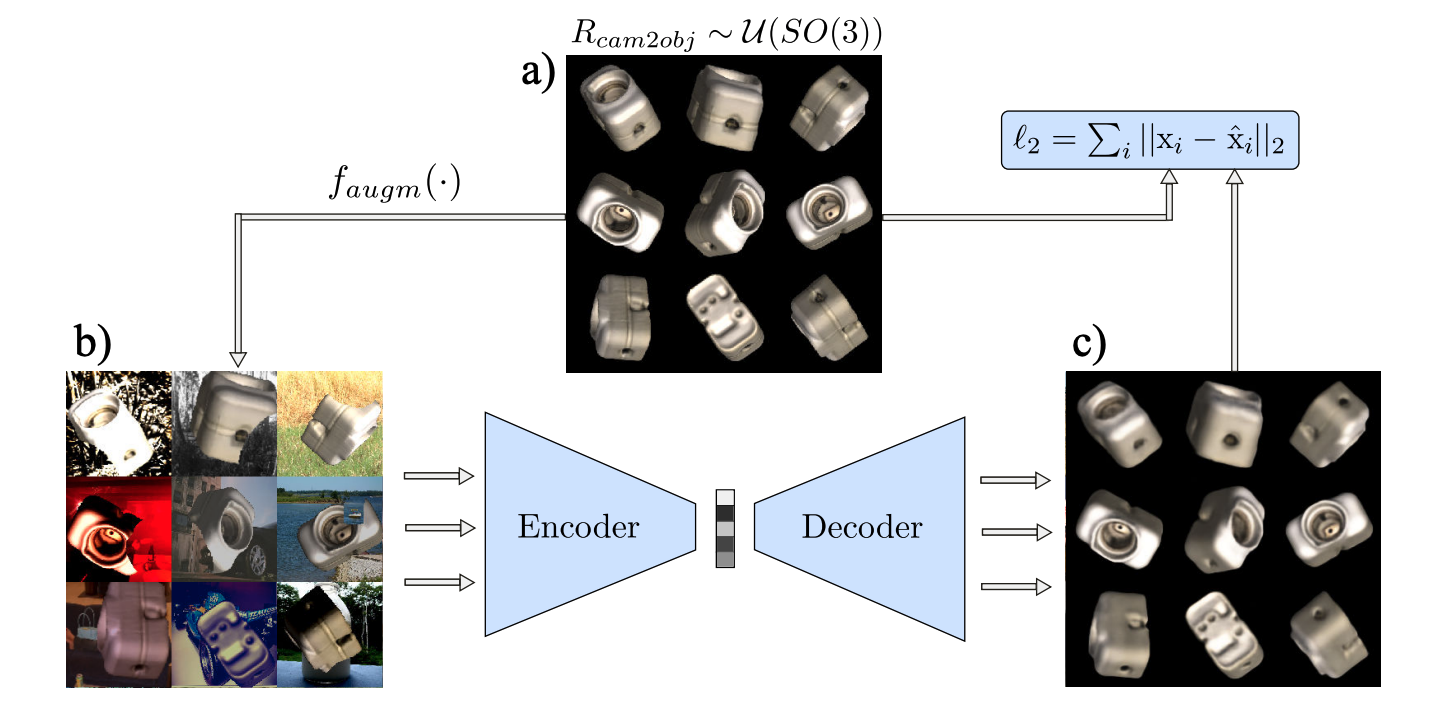
\includegraphics[width=1.0\textwidth]{img/c2/rel_b5.png}
        \bicaption{增强型去噪自编码器的结构和训练过程。图自~\citet{Sundermeyer_2018_ECCV}。}{Augmented Autoencoder and its training process. Figure is from~\citet{Sundermeyer_2018_ECCV}.}
        \label{c2_fig10}
    \end{figure*}

\section{基于噪声标签的语义分割}
基于噪声标签的语义分割作为弱监督的另一种类型,面临着标签中有一部分错误的问题,即噪声标签问题。如何有效利用好噪声标签,来训练得到鲁棒的语义分割网络,是该任务的核心问题。近来已有一些工作\citep{Zhu2019PickandLearnAQ,Xue2020CascadedRL,Zhang2020CharacterizingLE,Zhang2020RobustMI},在该任务上做了探索,并取得了一些进展。

对噪声标签的利用,需要模型具备评估标签质量的能力,以决定使用或丢弃哪些标签。正确的标签可以让模型充分训练,而噪声标签会干扰训练结果,甚至由于深度神经网络的较强的表征能力,模型会记住这些标签错误。除了设计方法尽可能选出正确标签来学习,另一方面,根据训练过程中学到的信息,错误标签也可以被纠正为正确标签,带来进一步的性能提升。

\citet{Zhu2019PickandLearnAQ} 在分割网络中引入了标签质量评估策略,来自动评估每张图像的标签质量,随后利用正确的标签进行训练。这篇文章提出了一个分割网络,其自动评估训练集里标签的相对质量,并使用好的标签来更新网络参数。自动评估的想法来自于标签与输入图像的一致性关系,噪声标签往往与输入样本有明显的冲突,这区别于同一批次中对比正确标签与输入样本的关系。此外还设计了一个过拟合控制模块,让网络在训练过程中尽可能地从精确标签中学习。过拟合控制模块可以确保有足够的可训练样本和避免过拟合。
    \begin{figure*}[tbp]
        \centering 
        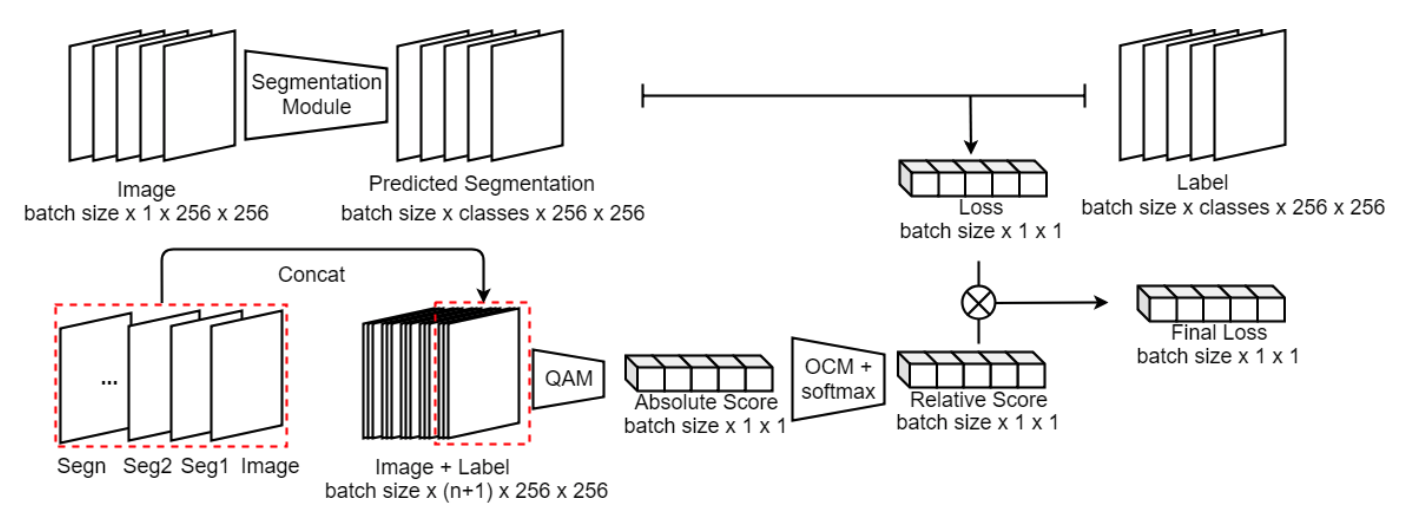
\includegraphics[width=1.0\textwidth]{img/c2/rel_c1.png}
        \bicaption{应用标签质量评估策略的端到端分割模型。图自~\citet{Zhu2019PickandLearnAQ}。}{The end-to-end architecture of the proposed label quality evaluation strategy. Figure is from~\citet{Zhu2019PickandLearnAQ}.}
        \label{c2_fig11}
    \end{figure*}

模型结构如图~\ref{c2_fig11}所示,该工作的中心目标是使用网络来计算同一批次中图像的相对质量分数,并找到存在于噪声标签中的冲突信息,利用这些信息,网络可以将噪声标签和正确标签区分开来。该模型由三个组成模块:分割模块、质量评估模块和过拟合控制模块。
训练过程中,与有正确标签的样本相比,有噪声标签的样本的预测分割会有较高的损失值,直接训练会干扰模型的学习能力和效果。为了对同一批次样本进行重新加权,质量评估模块和过拟合控制模块联合为每个输入产生相对权重,这个权重与分割模块计算的损失相乘,作为最终损失进行反向传播。这样,正确标签和噪声标签对模型的训练有不同权重的影响,使得模型能进行正确训练且具备抗噪声干扰能力。
分割模块是通用的生成语义分割的卷积神经网络,用以将输入图像通过多层特征提取和分辨率恢复产生分割预测。
质量评估模块也是一个卷积网络,但它将输入图像及其标签的拼接作为输入,为每张图像输出一个对应的质量评估分数,与分割模块平行运行。
过拟合控制模块在质量评估模块之后,为了防止前一个模块输出的评估分数的过拟合问题,以保证模型的训练稳定。它通过一个重缩放变换来调整评估分数。

在公开的生物医学分割 JSRT 数据集~\cite{Shiraishi2000DevelopmentOA}的实验表明,该方法优于基线方法,并且在不同的噪声水平下都能保持较高的准确性和良好的泛化能力。


为了更充分地利用标签信息,\citet{Xue2020CascadedRL} 提出了一种新的级联式的鲁棒学习框架。模型由三个独立的网络结构组成,这种设计能够从同级网络中有效学习信息。该框架包含两阶段,第一阶段通过模型选择机制选出正确标签的图像样本,通过分割损失最小化来训练网络。第二阶段则设计了一个带标签校正的联合优化框架,以逐步纠正错误标签并改进网络性能。
    \begin{figure*}[tbp]
        \centering 
        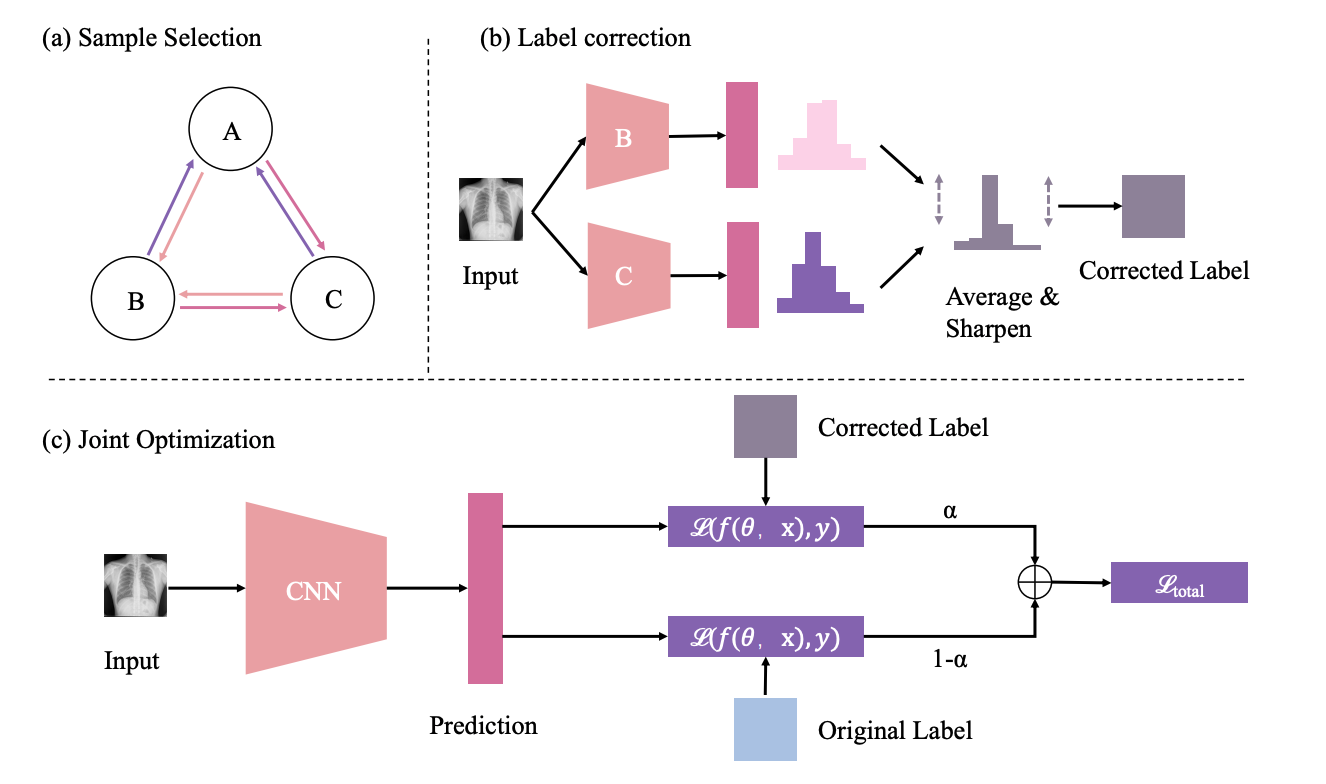
\includegraphics[width=1.0\textwidth]{img/c2/rel_c2.png}
        \bicaption{级联式鲁棒学习框架。图自~\citet{Xue2020CascadedRL}。}{Illustration of the pipeline of our cascaded robust learning framework. Figure is from~\citet{Xue2020CascadedRL}.}
        \label{c2_fig12}
    \end{figure*}
如图~\ref{c2_fig12},作者沿用了之前的鲁棒学习思路:选用高置信度的样本来更新网络可以提高对噪声标签的鲁棒性。所提的框架由三个独立而相同结构的网络组成。在第一阶段的训练过程中,选择不确定性较小的高置信样本来更新每个网络,因为这些样本大概率是正确标签。具体地,每个网络用于训练的样本由其他两个网络获得,首先排除预测结果不一致的样本,然后在低不确定性样本中,选择小损失值的样本。
然而,样本选择阶段只有部分样本可以用于训练,而无法充分利用标签信息。为了提高标签的利用效率,第二阶段设计了一个联合优化框架,用原始标签和修正标签共同训练网络。为了纠正有噪声的标签,作者设计了一个标签校正模块,校正标签由不同网络预测的平均值再通过锐化函数生成。
总之,通过这样一种级联的学习框架,这篇工作充分利用了噪声标签的信息,且避免了错误标签的干扰,提高了分割的准确性。
% 这篇工作在深圳医院收集的公开胸部 X 射线数据集进行了实验,结果表明,相比于之前的方法,这种基连的鲁棒学习框架在分割任务的准确性

% \citet{CL}

上述两篇工作都可以视为图像级别的的训练加权策略,这类方法将每幅图像的标签视为正确或噪声,并迭代选择或重新权衡图像样本。但是在重度的噪声环境下鲁棒性很差,因为它们无法充分利用每幅图像中具有正确注释的像素,为了解决这一局限性,另一类方法是将分割任务视为像素级的分类任务,进行像素级样本选择或标签校正。

\citet{Zhang2020RobustMI} 基于协作学习策略,提出了一种高效的三网络学习框架。其中两个作为教师网络,共同选择可靠的像素样本给第三个网络。三网络的设计能够保证选择样本的稳定性与可靠性,并且为平衡噪声与信息留下策略空间。为了便于选择可靠的样本,这篇工作根据两个网络输出的共识与差异设计了两种可行的策略。随后,选定的样本被送入第三个网络以更新其模型参数。通过这种方式,三个网络以协作的方式学习。
    \begin{figure*}[tbp]
        \centering 
        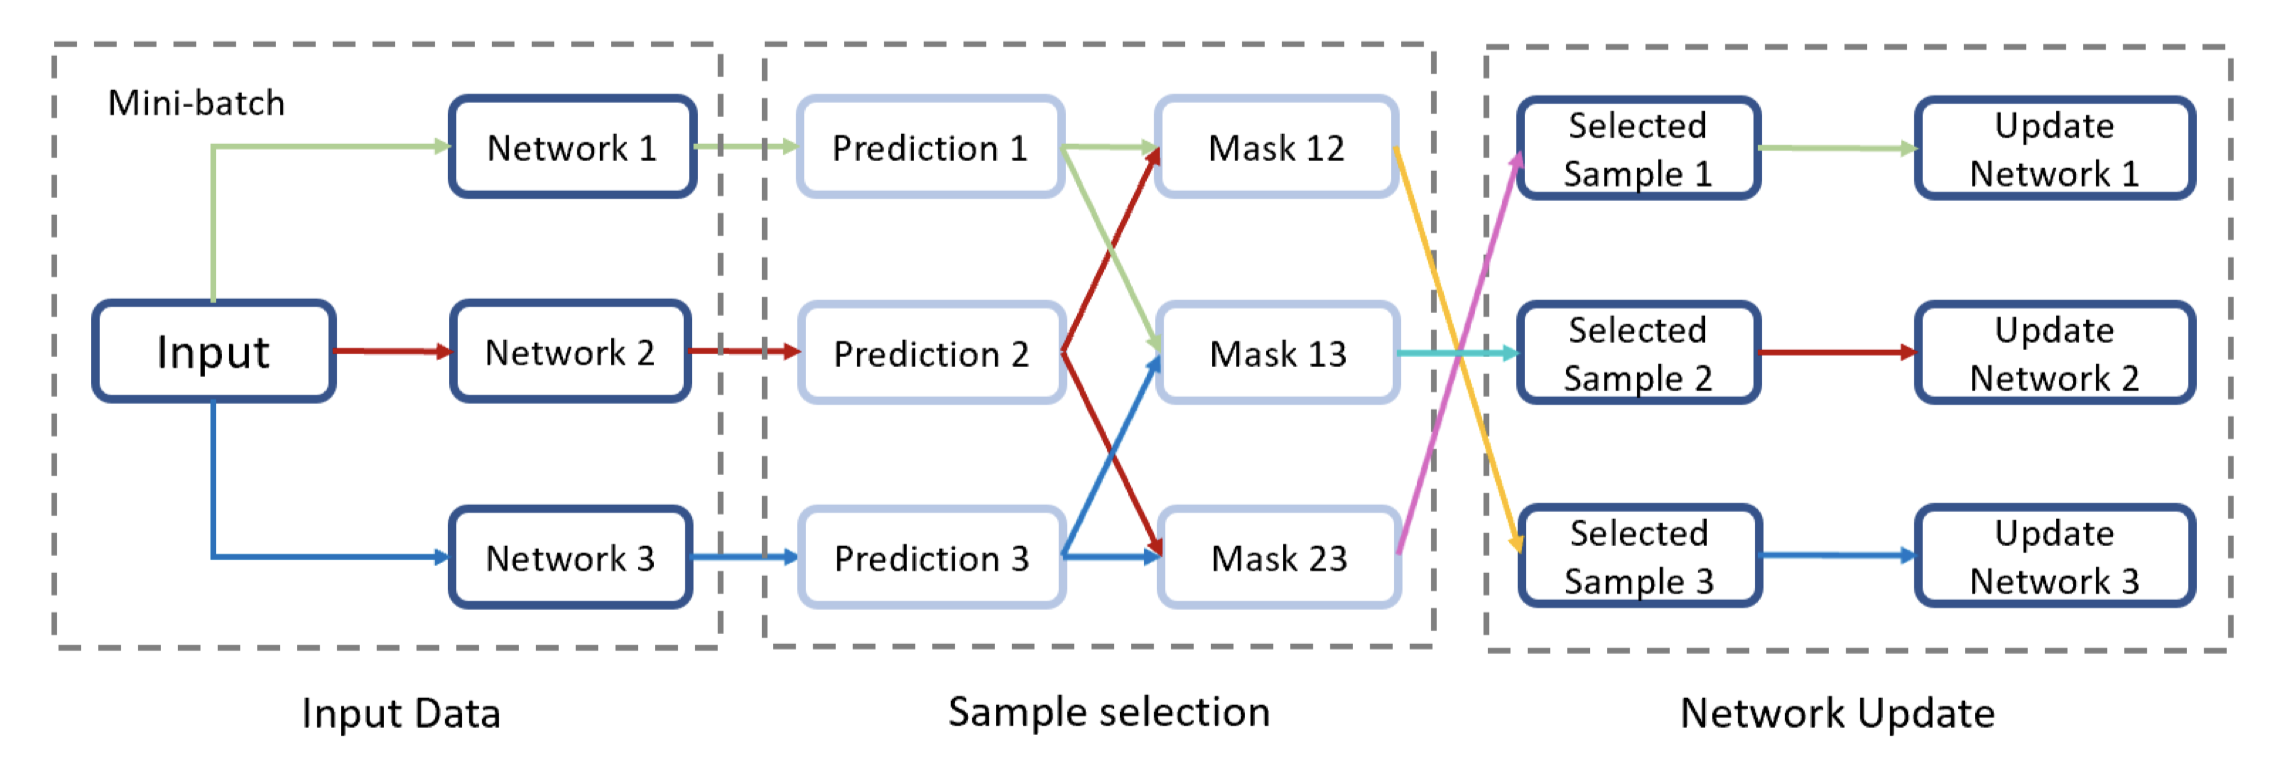
\includegraphics[width=1.0\textwidth]{img/c2/rel_c3.png}
        \bicaption{三网络协作学习框架,采用了像素级的样本选择策略。图自~\citet{Zhang2020RobustMI}。}{The pipeline of our Tri-network framework, which adopts the pixel-level sample selection strategy. Figure is from~\citet{Zhang2020RobustMI}.}
        \label{c2_fig13}
    \end{figure*}
模型框架如图~\ref{c2_fig13}所示,关键思想是同时训练三个网络,其中每一对网络都引导第三个网络从噪声标签中挖掘有用和可靠的信息。给定一个小批量的输入数据,分别送入三个网络,得到三种不同的预测图和相应的像素损失图。接下来,每一对网络根据其输出经样本选择策略选出可靠的像素,用以引导第三个网络的训练更新。在测试阶段,测试数据被送入三个训练好的网络,并将三个网络的输出合并后作为最终预测。

对于样本选择策略,该工作提出两种选择标准:基于共识的选择或基于差异的选择。这两个标准在处理有噪声标签的分割问题上都被证明是有效的。
基于共识的选择,是对网络预测的共识。对于每个小批数据,一对网络产生两组像素级预测图,通过计算网络预测和噪声标签之间每个像素的损失,可以得到每个网络相应的置信度图(也是损失图)。一个设置好的损失值阈值,会将每个置信度图二元化,其中 1 表示高置信度(对应小的损失值),0 表示低置信度(对应大的损失值)。基于两个网络的二元置信图,可以计算得到共识图。共识图中有两种像素:两个网络共同的高置信度像素(被认为有干净标签),和共同的低置信度像素(被认为难学习而有信息量的样本)。这两种像素被送入第三个网络训练,而其他不一致置信度的像素不予考虑。
基于差异的选择,与共识策略类似。首先计算每个网络预测的像素级损失图,然后计算两个损失图的差并取绝对值。在此策略中,通过选择一定比例的较大的损失差异像素,来挖掘有用的信息。选中的像素送入第三个网络更新其参数。


\section{本章小结}
本章中我们对相关的工作进行了总结并分析,包括基于弱标签的语义分割、自学习方法、去噪自编码器、基于噪声标签的语义分割等内容。为开展我们的研究工作奠定基础。


\chapter{基于弱标签的语义分割}
% 在本文中,我们提出了一种新的三维物体分割的弱监督学习策略,以解决上述的挑战。我们的主要想法包括两个方面。首先,我们提出了一种自学习方法,通过物体样本增强的方法,来捕捉目标物体类别的三维形状先验。随后,我们将这种学习到的形状先验纳入具有形状感知的分割网络的训练过程。另外,我们采用了一个稀疏的弱标注方案,以更好地利用物体掩膜的空间连续性,并在不增加整体标注成本的情况下促进形状上下文的学习。
%为了实现这一目标,我们设计了一个由两个主要模块组成的深度神经网络:一个是标准的语义分割网络,它从三维输入图像中产生一个初始的三维分割掩膜;另一个是形状去噪网络,它对初始分割掩膜进行改进并输出一个最终的三维分割。为了训练深度网络,我们首先引入一种稀疏的弱标注方案,在该方案中,我们只标注三维数据的一个特定的二维图像切片的子集(可以将三维图像数据视作一系列连续的二维图像切片),同时对每张二维图像,我们设计了一种混合式弱标签,它结合了前景涂鸦和目标物体的一个宽松边界框。给定这样的弱标注形式,我们为前述的网络模型设计了一个迭代学习框架,交替进行像素级标签生成和网络参数更新。

在本章,我们为基于弱标签的语义分割提出一种新的结合形状先验的学习策略。我们的目标是利用物体的形状先验设计更有效的弱监督分割框架,并将其纳入训练过程。为此,我们探索自学习方法,从仅有弱标签的训练数据中学到目标类别的形状先验。更进一步,我们对比了不同的弱标注策略,并提出一种新的混合式标注方法,来为弱监督学习提供更有效的训练信息和更好的性能。我们采用了迭代学习的方法,来逐步地提升分割效果,直至模型参数收敛。

% 各小节介绍
本章内容来自笔者的一篇合作的已发表工作~\cite{he2021weakly},笔者的主要贡献是捕捉形状先验的自学习方法、稀疏的混合式标签策略、模型与训练方法的实现。
本章结构分为以下五个部分。在第一节我们对基于弱标签的语义分割任务进行介绍,第二节介绍我们提出的结合形状先验的弱监督分割模型。然后,在第三节我们提出新的高效的稀疏弱标注策略,随后在第四节详细介绍了模型的训练方法,特别是自学习形状模型的策略。第五节为实验部分,包括实验设置、实验细节、定量结果、定性结果、消融实验等。最后一节是本章总结。

\section{问题概述}
医学图像的分割任务如图~\ref{c3_fig1}所示,左侧为二维图像及其分割结果,右侧为三维图像及其三维分割可视化(三维图像由一系列连续的二维图像堆叠成统一的整体)。
特别地是,基于弱标签的语义分割,其训练样本采用了弱标签而非全标签的形式。
给定一个输入的三维体积图像 $\mathbf{I} \in \mathbb{R}^{H \times W \times D}$,我们的目标是估计其分割掩膜 $\mathbf{M} \in \mathcal{S}^{H \times W \times D}$,其中 $H$ and $W$ 是图像切片的高度和宽度,$D$ 则是组成三维图像的切片数目。$\mathcal{S} = \{0, 1\}$ 是语义标签集,其中 $0$ 表示背景类,$1$ 为前景类。
训练数据集 $\mathcal{D} = \{\mathbf{I}^n, \mathbf{Y}^n\}_{n=1}^N$,其中 $\mathbf{Y}^n \in \mathcal{S}'^{H \times W \times D}$ 是 $\mathbf{I}^n$ 对应的弱标签, $\mathcal{S}' = \mathcal{S} \cup \{u\}$ 且 $u$ 代表无标签像素,$N$ 是训练数据样本的数目。
在本文中,我们关注二分类分割问题,即只有前景类别和背景类别。我们的方法可以通过单独处理每个类别来应用在多分类问题。

这个工作中我们的核心思想是,从弱标签中得到一个自学习的形状先验,然后利用这个形状先验来进一步进行形状去噪和改进。为了实现这一目标,我们设计了一个由两个主要模块组成的深度神经网络:一个语义分割模块和一个形状去噪模块。我们首先用语义分割模块在输入图像上预测一个初始的粗分割掩膜,然后形状去噪模块在初始掩膜上应用自学习的形状先验来进行去噪和改进。为了进一步利用形状先验来改进模型,我们采用了一种迭代学习框架,它在生成伪标签和更新模型参数之间迭代进行。我们的模型概览见图~\ref{fig:model}。


    \begin{figure*}[tbp]
        \centering 
        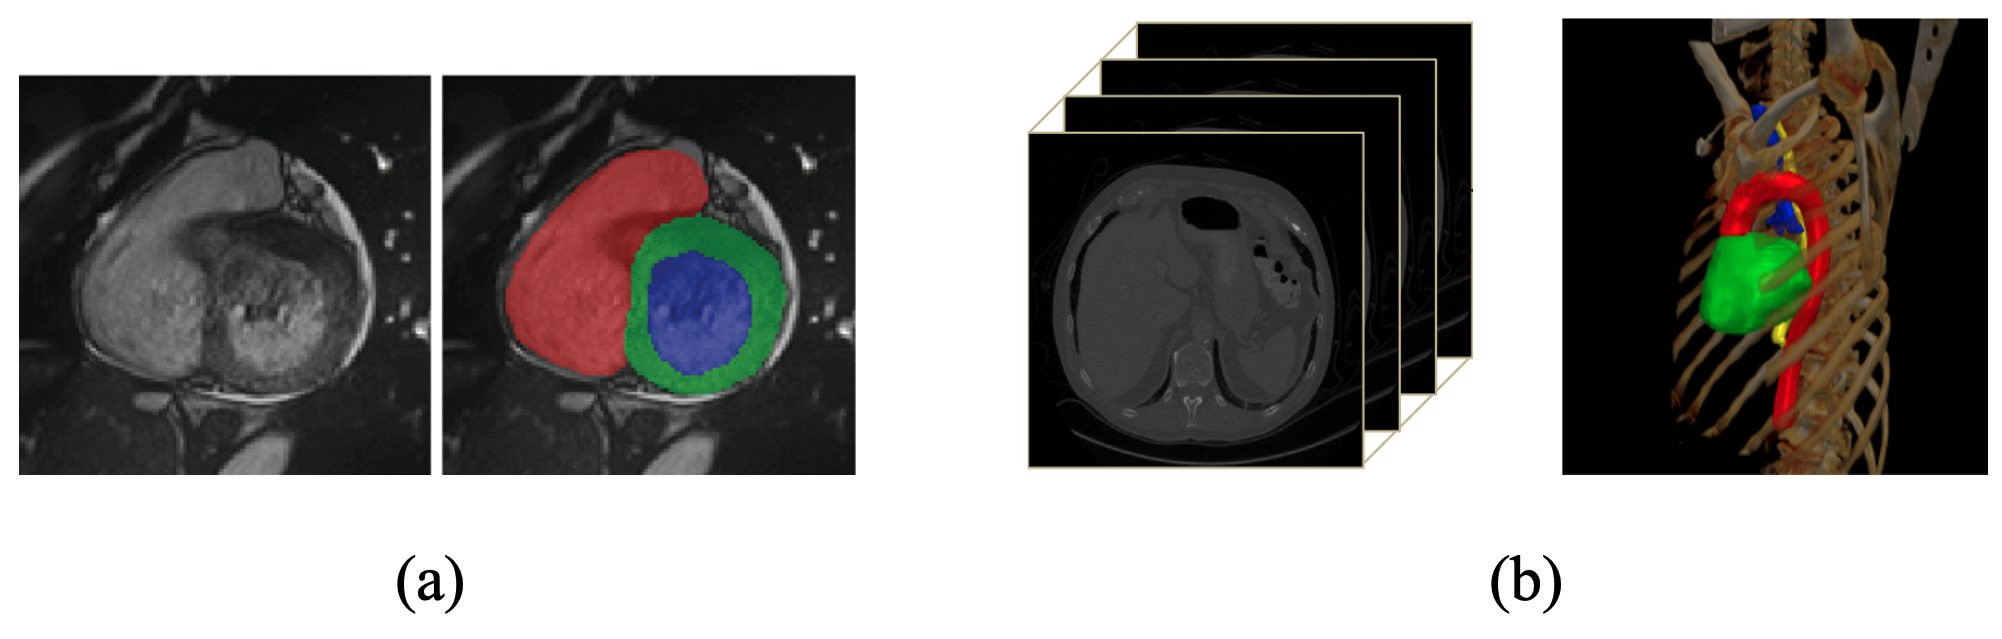
\includegraphics[width=1.0\textwidth]{img/c3/c3_1.png}
        \bicaption{医学图像的语义分割任务示例。左侧为二维图像与分割标签,右侧为三维图像(由一系列连续的二维图像组成)及其标签。}
        {Examples of medical image semantic segmentation. (a) 2D image and its segmentation label. (b) 3D image and its segmentation label.}
        \label{c3_fig1}
    \end{figure*}

    \begin{figure*}[t!]
        \centering 
        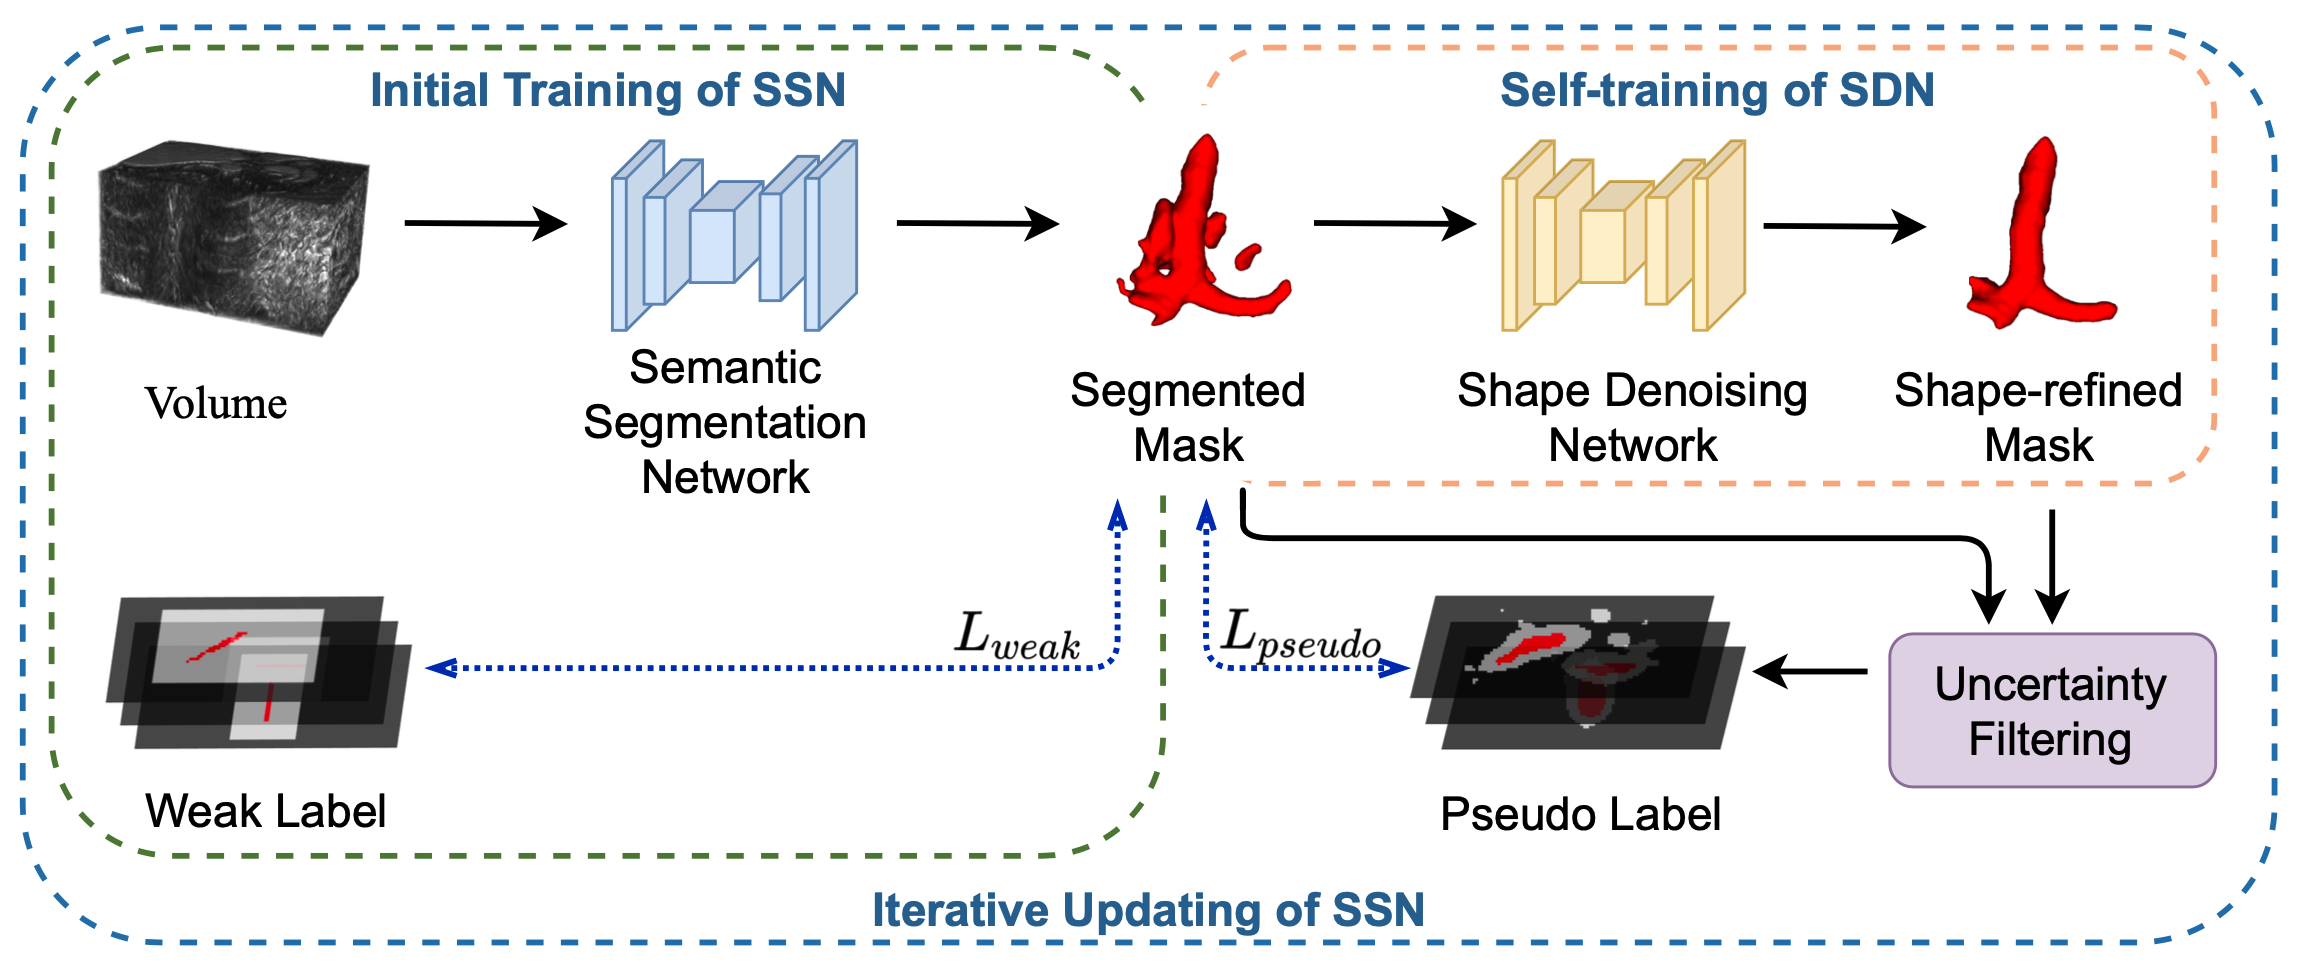
\includegraphics[width=1.00\textwidth]{img/c3/b_model_shape.png}
        \bicaption{弱监督语义分割模型概览。我们的模型由两个主要模块组成:语义分割网络和形状去噪网络。语义分割网络从输入的体积图像中预测出一个初始的分割掩膜,并由其后形状去噪网络进一步完善,作为最终输出。我们采用一种迭代训练的方法来训练模型。}
        {The overview of our method. Our model consists of two main modules: Semantic Segmentation Network (SSN) and Shape Denoising Network (SDN). Our SSN predicts an initial segmented mask from the input volumetric image, which is further refined by our SDN as final output. To train our model, we propose an iteraitve learning strategy.}
        \label{fig:model}
    \end{figure*}


\section{模型设计}
在本节我们详细介绍模型中的两个主要模块:语义分割网络和形状去噪网络。

\textbf{语义分割网络} \quad 语义分割网络 $\mathcal{F}_{SSN}$ 用来产生一个初始的粗分割掩膜,它将一个体积图像 $\mathbf{I}$ 作为输入,并输出一个概率图 $\mathbf{P}_s \in [0,1]^{H\times W\times D}$,表示每个像素属于前景的置信度。由 $\mathbf{P}_s$ 我们可以得出初始的前景分割掩膜 $\mathbf{M}_s$:
\begin{align}
    \mathbf{P}_s = \mathcal{F}_{SSN} (\mathbf{I}; \Theta), \mathbf{M}_s = \mathds{1} (\mathbf{P}_s > 0.5)
\end{align}
其中 $\Theta$ 表示 $\mathcal{F}_{SSN}$ 的参数,而 $\mathds{1}(\cdot)$ 是一个指示函数。
我们用 nnU-Net~\citep{isensee2019automated} 来实例化我们的语义分割网络,它是医学图像语义分割的最先进而广泛的模型结构。
% 可扩展:将 模型的具体设计可再讲一段,从附录 C 里取出。


\textbf{形状去噪网络} \quad 我们设计了一个形状去噪网络 $\mathcal{F}_{SDN}$ 来编码一个统一的形状先验,然后应用于初始的粗分割掩膜上进行形状改进。形状去噪网络的思想借鉴自去噪自编码器\citep{vincent2010stacked}和增强自编码器\citep{Sundermeyer_2018_ECCV}。去噪自编码器将图像编码为对噪声不敏感的隐向量,以表示原始的干净图像。增强自编码器产生输入图像中物体的方向编码,而对其他变换和环境条件具有不变性。与这些旨在为图像或物体方向提供代表性向量表征的方法不同,我们的目标是将输入的粗分割掩膜中恢复为干净而完整的形状。
给定语义分割网络输出的初始掩膜 $\mathbf{M}_s$,我们的形状去噪网络隐式地施加了自学习的形状先验约束,并输出一个干净的形状改进的分割掩膜:
\begin{align}
    \mathbf{P}_d = \mathcal{F}_{SDN} (\mathbf{M}_s; \Omega), \mathbf{M}_d = \mathds{1} (\mathbf{P}_d > 0.5)
\end{align}
其中 $\Omega$ 表示 $\mathcal{F}_{SDN}$ 的参数。由于我们的输出目标是最终的分割掩膜,而不是隐向量表示,我们的 $\mathcal{F}_{SDN}$ 采用了与 $\mathcal{F}_{SSN}$ 相同的 U-Net 结构,这种设计使得形状去噪网络在中间瓶颈层也保持较大的空间分辨率,并包含跳跃连接以捕捉更多的分割细节。

\section{弱标注策略}
为了更好地利用物体掩膜的空间连续性并促进形状上下文的学习,我们为三维体积分割任务设计了一个稀疏的弱标注策略。
标注方案包含两个方面,切片选择和混合式标签策略。三维图像由一系列连续的二维切片组成,但我们不需要逐切片地标注,而是对切片选择性标注。对切片选择方法,我们先选择标注每个前景物体的起始和结束的切片,因为它们包括 $z$ 轴上的重要边界信息。除了这两个切片,我们还随机标注它们之间切片的一个子集。在这项工作中,我们研究了多个标注比例设定,分别是 10\%、30\%、50\%和100\%的前景切片标注比例。
另一方面,我们为二维切片设计了一种混合式标签,它包括在前景物体区域的一条长轴涂鸦和一个包围所有前景像素的松散边界框。具体来说,对于长轴涂鸦,标注者只需在前景物体内部的边界附近点击两个点,就可以根据两段点自动形成一条线。对于松散的边界框,标注者只需要点击位于左上角和右下角的两个点,就可以自动形成一个矩形框。
值得注意,我们的混合式标签并不需要对边界点进行精确的定位,而只需要标注者大致指出前景的内部和外部区域。与传统的涂鸦式标签或紧致的边界框相比,混合式标签可以提供丰富的背景信息和粗略的定位,以及前景像素标签,而每个 2D 切片只需四个标注点。为了模拟我们的弱标注策略,我们从全掩膜中生成混合式标签。图~\ref{fig:weak_annotation}中显示了一些例子。
% 可扩展:将弱标签在附录B中的两段内容拿出来扩展。

    \begin{figure*}[tbp]
        \centering 
        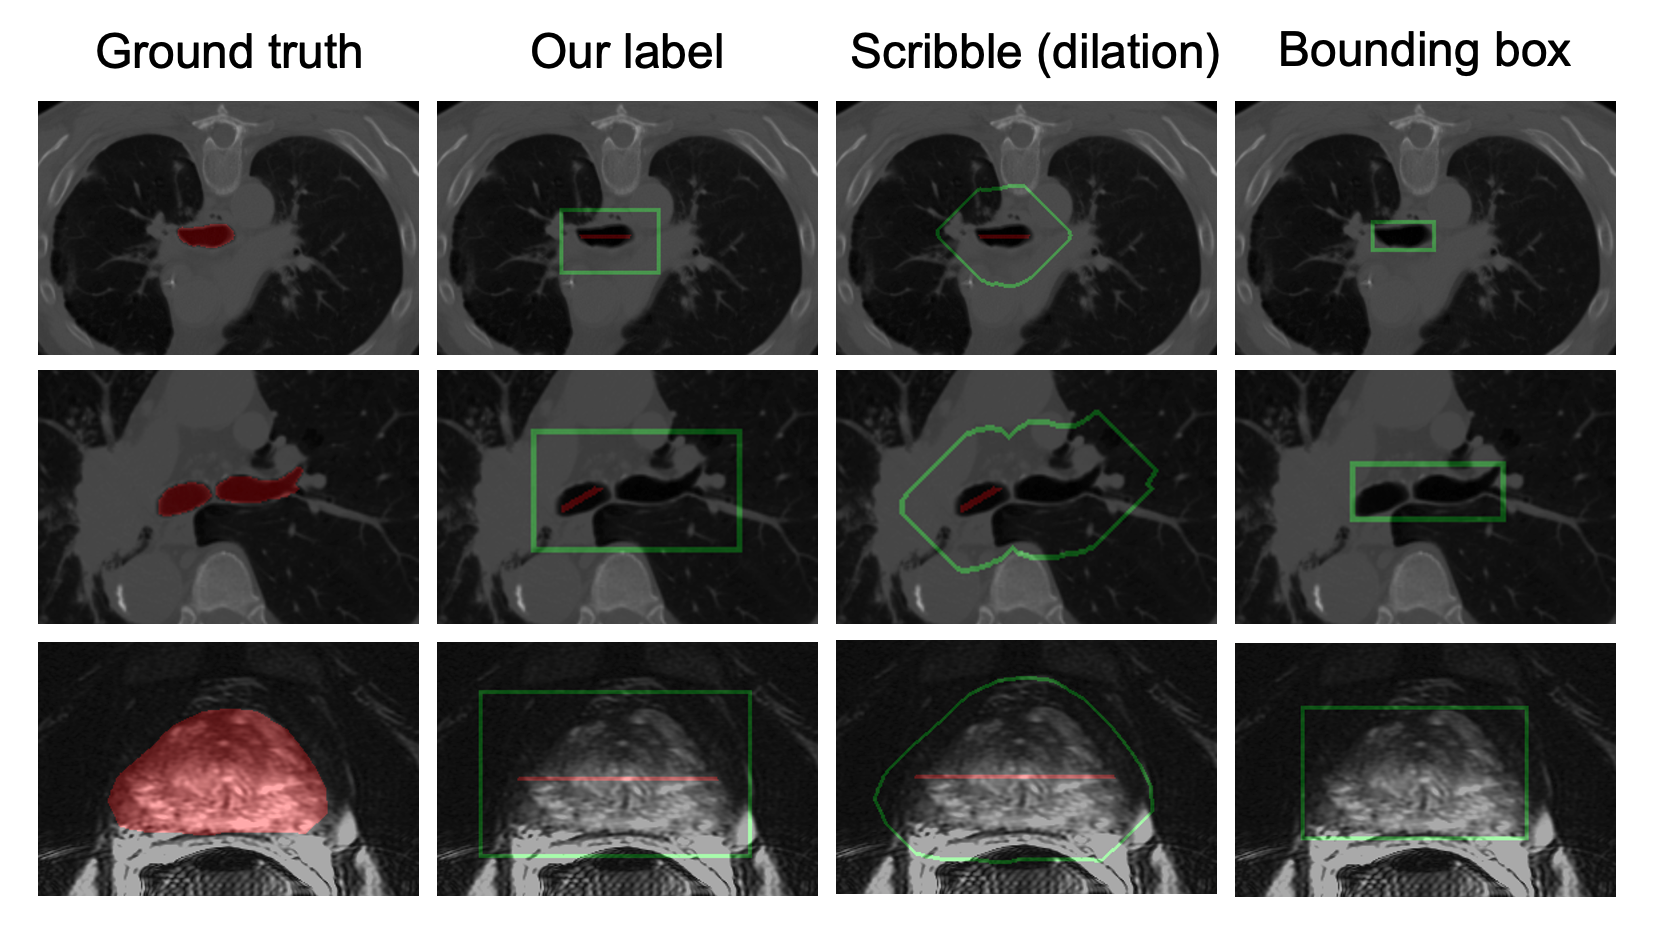
\includegraphics[width=1.0\textwidth]{img/c3/c_weak_annotation3.png}
        \bicaption{不同标注方法的示意图,分别在气管的连通和分叉区域(第一、二行)和前列腺(第三行)的图像上展示。第一列为精确的全标注,第二列为我们的混合式标注方法,第三列是涂鸦式标注(由前景区域膨胀操作模拟生成),第四列是紧致的边界框标注。}
        {We show different annotations for trachea (first row: connected part, second row: separate part) and prostate (last row). Four rows show groundtruth, our hybrid label, scribble and bounding box, respectively. Scribble (dilation) denotes generated scribble by foreground mask dilation.}
        \label{fig:weak_annotation}
    \end{figure*}

\section{模型训练}
为了有效地训练提出的模型,我们采用了一个迭代学习框架,它迭代地生成伪标签和更新模型参数。为了生成初始伪标签,我们首先初始化训练模型中的语义分割网络和形状去噪网络。然后,我们结合语义分割网络和形状去噪网络的输出,并通过不确定性过滤机制来计算生成伪标签。两个输出的结合是为了消除噪声并在模型更新中引入学到的形状先验。
接下来,我们依次介绍语义分割网络的训练、自学习的形状去噪网络的训练、不确定性过滤机制的伪标签生成,以及最终的模型更新。

\paragraph{训练语义分割网络}
我们首先在弱标签上训练语义分割网络,以提供初始分割掩膜。初始掩膜会作为形状去噪网络的重要训练信息。
给定输入图像和相应的弱标签,我们使用有标签像素上的加权交叉熵来训练语义分割网络:
\begin{align}
    \mathcal{L}_{SSN} (\Theta) = \mathcal{L}_{wce} (\mathbf{P}_s, \mathbf{Y})
\end{align}
在我们的混合式标签中,边界框外的区域全部可视为背景像素,而前景只有涂鸦式标签覆盖的像素。由于弱标签中前景和背景的极大不平衡,我们在损失函数中采用了自动加权策略,来平衡前景和背景的影响。实验表明,与固定的加权比例相比,我们的自动加权策略更加稳定,对不同的数据集有更好的泛化性。
具体来说,对于每个有 $N_b$ 个有标签背景像素和 $N_f$ 个有标签前景像素,我们计算损失为
\begin{align}
    (\frac{1}{N_b} \sum^{N_b}_{i} l_i + \frac{1}{N_f} \sum^{N_f}_{j} l_j) / 2
\end{align}
其中 $l_i$ 表示第 $i$ 个像素的交叉熵损失。

\paragraph{自训练的形状去噪网络}
不同于之前的去噪模型学习方法,我们用自学习的策略来训练形状去噪网络。\citet{vincent2010stacked} 对输入图像应用人工的随机噪声增强,并重建对应的干净图像目标。\citet{Sundermeyer_2018_ECCV} 提出了一种域随机化技术,以模拟真实相机捕捉的环境和传感器变化。他们利用这种技术来增强输入合成图像,并重建除方向外其他因素不变性的图像。

对我们的问题,一个重要的区别是,没有用于自学习的完整掩膜标签。即没有可用的训练目标标签,这里是形状完整的标签。
一个可能的解决方案是使用数字合成的形状模型,但对不同的数据集可能有很大的域差距,特别是对医学分割中的掩膜。为了避免这种域差距,我们提出了一个自学习策略:首先用弱监督分割模型中的语义分割网络提取出自学习的形状表示,然后用这样的形状表示来训练形状去噪网络。其基本假设是,我们初训练的语义分割网络能够在训练集中的某些实例上产生高于平均水平的分割掩码,因此能够提供形状质量较好的分割掩膜,来帮助改善其他形状质量较差的掩膜。为此,我们首先计算训练集中每个 $\mathbf{P}_s$ 的平均前景概率,作为每个分割掩膜 $\mathbf{M}_s$ 的置信度,然后选取置信度最高的分割掩膜作为我们自学的表示 $\mathbf{M}^*$ 来训练形状去噪网络。

形状去噪网络的作用是去除形状层面的噪声,为了训练这种能力,我们不是在输入掩膜中加入通常的随机噪声,而是根据初始化的语义分割网络输出的错误模式的观察,特别设计形状层面的噪声增强方法。
我们将初始分割掩膜的典型错误模式总结为三类。
\begin{enumerate}
    \item 过度平滑的区域。这是由于边缘区域的监督信号较少,模型无法区分准确边缘所致。
    \item 表面错误附着的斑块。仅根据视觉特征,容易把其他相近的区域也预测为目标物体的一部分。
    \item 轴向上超出前景起始和结束切片的多余预测。根据相近的视觉特征和连续性,容易产生错误的轴向物体延长。
\end{enumerate}
这些形状错误模式主要是因为在弱标签中没有明确的边界监督,而邻近的物体区域可能与目标物体有相似的强度或纹理特征。

为了使我们的形状去噪网络具备处理上述错误的能力,我们设计了三种相应的噪声增强操作。(1) 形态学的闭操作;(2) 形态学的膨胀;(3) 边缘切片的形状延伸。例子如图~\ref{fig:shape_aug}所示。
    \begin{figure*}[tbp]
        \centering 
        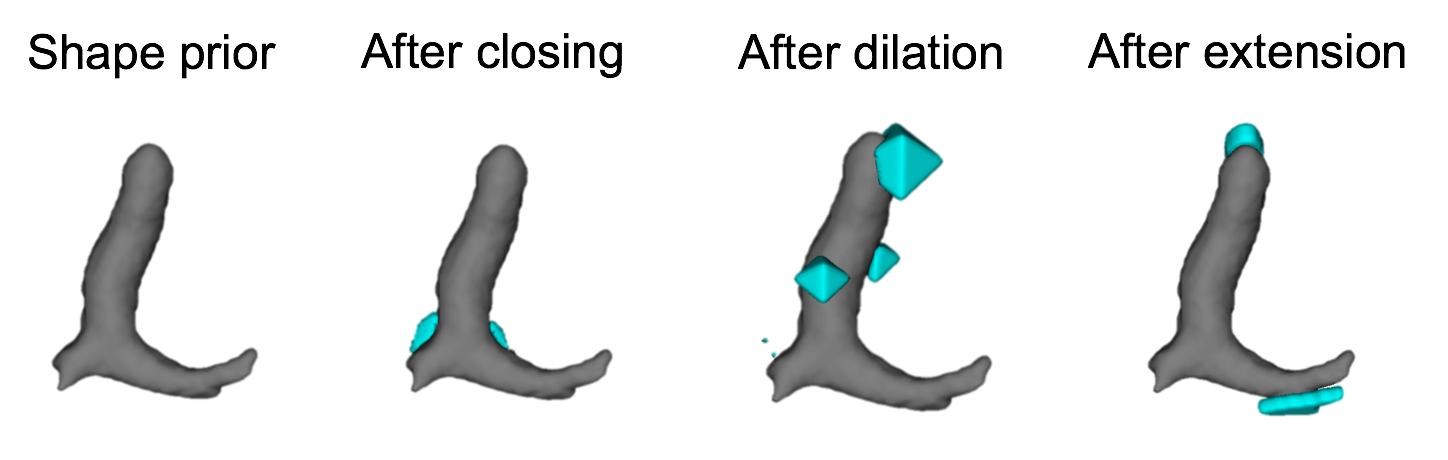
\includegraphics[width=1.0\textwidth]{img/c3/b_shape_aug2.png}
        \bicaption{气管分割上,我们自学习的形状表示和对应的噪声增强的示意图。}
        {An example of our self-taught shape representation and corresponding augmentation effect on trachea.}
        \label{fig:shape_aug}
    \end{figure*}
为了充分扩充形状去噪网络的训练数据集,我们还应用了空间变换,包括旋转、平移和缩放。这样可以捕捉丰富的位置和尺寸变化,有助于学习隐式的形状流形。我们将自学习的形状表征M∗增强为M∗,并训练我们的SDN来重建具有交叉熵损失的干净面具M∗。
我
们应用空间转换,包括旋转、平移和缩放,以捕捉丰富的位置和尺寸变化,这有助于学习潜在的形状流形。我们将自学的形状表征 $\mathbf{M}^*$ 增强为 $\mathbf{\hat{M}}^*$ 作为输入,并训练形状去噪网络来重建干净的掩膜 $\mathbf{M}^*$:
\begin{align}
    \mathcal{L}_{SDN} (\Omega) = \mathcal{L}_{ce} (\mathcal{F}_{SDN} (\mathbf{\hat{M}}^*; \Omega), \mathbf{M}^*)
\end{align}

\paragraph{不确定性过滤}
为了利用自学习的形状先验来进一步改进我们的模型并去除预测标签的噪声,我们设计一个不确定性过滤机制,从语义分割网络和形状去噪网络的概率预测中生成伪掩膜标签。具体地说,我们首先计算语义分割网络和形状去噪网络各自输出的分割掩膜,对二者取交集,然后根据语义分割输出中P s的每个像素的确定性,

不确定性过滤 为了结合自学的形状先验来进一步改善我们的模型并去除噪音,我们用一个简单的不确定性过滤机制从SSN和SDN的预测中生成伪掩码。具体来说,我们首先计算SSN的分割面具和SDN的形状重构面具的交集,然后根据语义分割输出 $\mathbf{P}_s$ 中每个像素的置信度,应用基于不确定性的过滤。我们为前景($\mathbf{Y}_{fg}$)和背景($\mathbf{Y}_{bg}$)独立计算伪标签掩膜,
\begin{align}   \label{eq1}
    \mathbf{Y}_{fg} &= \mathbf{M}_s * \mathbf{M}_d * \mathds{1} (\mathbf{P}_s > \sigma_{fg})
\end{align}
\begin{align}   \label{eq2}
    \mathbf{Y}_{bg} = (1-\mathbf{M}_s) * (1-\mathbf{M}_d) * \mathds{1} (\mathbf{P}_s < \sigma_{bg})
\end{align}
其中 $\sigma_{fg}$ 和 $\sigma_{bg}$ 是前背景各自的不确定性阈值。
最后的伪标签 $\mathbf{Y}_p$ 结合了 $\mathbf{Y}_{fg}$ 和 $\mathbf{Y}_{bg}$,
\begin{align}
    \mathbf{Y}_p &= \mathds{1}(\mathbf{Y}_{fg} = 1) + u * \mathds{1}(\mathbf{Y}_{fg} = 0) * \mathds{1}(\mathbf{Y}_{bg} = 0)
\end{align}
其中无标签的像素设置为 $u$。

\paragraph{模型更新}
得到生成的伪标签 $\mathbf{Y}_p$,我们通过最小化两项加权的交叉熵损失来更新模型参数 $\Theta$ :分割输出概率 $\mathbf{P}_s$ 相对于原始的弱标签和生成的伪标签,
\begin{align} \label{eq3}
    \mathcal{L} (\Theta) = \lambda_w \mathcal{L}_{wce} (\mathbf{P}_s, \mathbf{Y}) + \lambda_p \mathcal{L}_{wce} (\mathbf{P}_s, \mathbf{Y}_p)
\end{align}
其中 $\lambda_w$ 和 $\lambda_p$ 是各自相应的损失权重。
在迭代学习中,我们冻结了形状去噪网络的参数 $\Omega$。这是根据实验观察,更新 $\Omega$ 并不能带来进一步的改善。主要因为我们自学习的形状表示已经有相对较好的质量,而且设计的形状噪声增强足够充分,可以捕捉到各种错误模式。


\section{实验}
我们在两个公开的基准上评估了我们的方法,它们分别具有不同的形状,包括 SegTHOR\citep{trullo2019multiorgan}中的气管和 PROMISE12\citep{Litjens2014EvaluationOP}中的前列腺。在每个数据集上,我们与使用不同弱标签的最先进的方法进行比较。
下面我们首先在~\ref{sec:dataset}节介绍数据集信息,在~\ref{sec:detail}节介绍实现细节。然后,我们在~\ref{sec:res1}节介绍了与其他方法比较的定量结果和定性结果,并且在~\ref{sec:detail}节中介绍了完整的消融实验对比。最后,我们在~\ref{sec:extension}对方法中的弱标签和自学习形状模型进行了拓展讨论。
% 此外,我们在附录F中对我们的SDN进行了进一步的分析,以更好地理解形状去噪机制,并在附录G中讨论了我们的失败案例和潜在的未来工作。

\subsection{实验数据集} \label{sec:dataset}

\paragraph{SegTHOR挑战赛}
SegTHOR挑战赛\footnote{https://competitions.codalab.org/competitions/21145}\citep{trullo2019multiorgan}由60个胸部CT扫描图组成,来自被诊断为肺癌或霍奇金淋巴瘤的患者。这个数据集的所有扫描图像的尺寸为$512\times512\times(150-284)$,切面内的间距从 0.90 毫米到 1.37 毫米不等,切面间的间距从 2 毫米到 3.7 毫米。我们对数据集划分如下:将 40 份公开可用的扫描图分成 30 份作为训练,10 份用于验证,并将 20 份测试数据的结果上传官方网页在线评估。这个数据集包含四个器官:心脏、主动脉、气管和食管。我们在气管上进行实验,因为它更具有挑战性和代表性的器官形状。

% \paragraph{左心房数据集}
% 左心房数据集来自2018心房分割挑战赛\footnote{http://atriaseg2018.cardiacatlas.org/}。它包含100对三维钆增强的 MR 成像扫描(GE-MRIs)和对应的左心房分割掩膜。所有扫描都是各向同性的,其间距为 $0.625\times0.625\times0.625 mm^{3}$。每个病人的 MRI 图像的切面分辨率不同,而 Z 轴上都是 88 张切面。我们将 100 个扫描图分成 60 个用于训练,20 个用于验证,20 个用于测试。

\paragraph{PROMISE12挑战赛}
PROMISE12挑战赛\footnote{https://promise12.grand-challenge.org}\citep{Litjens2014EvaluationOP}包含 50 个横向 T2 加权 MR 图像,采用多种扫描协议,其分割目标前列腺位于图像的中央区域。这个数据集中的所有病例都是各向异性的,间距$2\times0.27\times0.27 mm^{3}$ 到 $4\times0.75\times0.75 mm^{3}$。我们采用与\citet{kervadec2020bounding}相同的设置,将 50 个扫描图分成 40 个用于训练,10 个用于验证。由于在线测试已不再支持,我们报告验证部集上的结果。

\subsection{实现细节} \label{sec:detail}

有些数据集(如SegTHOR)中的三维图像尺寸过大,直接作为模型输入需要大量的计算资源和时间,十分低效。
为了让目标物体的三维图像适应分割模型的输入,我们采用了基于弱标签的裁剪数据的预处理方法。具体来说,我们首先将体积图像重新取样到相同的体素间距,然后根据它们的中心对齐所有的训练样本,并将它们扩充到相同的大小,最后从所有样本中裁剪出一个统一的立方体,它是所有弱标注像素的交集所构成立方体的 1.2 倍。所有在我们的松散边界框外的像素,以及在起点和终点切片之外的像素,都被视为背景标签。

对于我们在训练形状去噪网络时的噪声增强,详细的处理如下。(1) 闭操作。我们对目标形状应用标准的形态学闭操作,即首先进行膨胀,然后进行腐蚀。闭操作提供了过度平滑的掩膜,这是气管和左心房的一个常见错误。(2) 膨胀。我们首先随机选择一个靠近掩膜边界的点作为中心,然后用一个范围内的随机迭代次数来膨胀。对于各向异性的数据集如前列腺,我们基于二维切片膨胀,而对于各向同性的数据集,我们采用三维膨胀。(3) 边缘切片的形状延伸。我们通过在 Z 轴上复制一些前景起始或结束的切片来延伸掩模。默认情况下,我们采用概率为 0.2 的随机空间变换,以丰富形状变化。

训练方法如下。参考\citet{isensee2019automated},我们采用相同的图像增强方法和深度监督模型方法训练,批大小为2。我们使用 SGD 优化器来训练。
对于初始化,我们用 1e-2 的初始学习率训练语义分割网络,并在多项式衰减策略下将其衰减到 1e-3,持续 200 轮。为了训练形状去噪网络,我们使用 1e-2 的固定学习率训练 100 轮。在迭代学习中,我们对不同的数据集使用不同的训练参数。在不确定性过滤中,对于每个体积图像,我们首先对预测的分割置信图 $\mathbf{P}_s$ 中的像素按置信度进行排序,然后设置前景不确定性阈值 $\sigma_{fg}$ ,以过滤掉置信度较低的部分。这个前景过滤比例 $\sigma_{fg}$ 对气管设为70\%,对左心房和前列腺的设为50\%。相应地,每个数据集的背景过滤比例 $\sigma_{bg}$ 被设定为  $2\sigma_{fg}$。
在模型参数更新中,对于气管,我们将损失权重($\lambda_w$, $\lambda_p$)设置为(1, 100),并以 1e-3 的学习率再训练我们的模型最多 300 次。对于前列腺,我们设定($\lambda_w$, $\lambda_p$)为(0.1, 10),学习率为 1e-2。对于左心房,我们设定($\lambda_w$, $\lambda_p$)为(0.1, 10),学习率为1e-3。


\subsection{实验结果} \label{sec:res1}

实验比较了基于所提出的混合式标签的我们的方法,和最近的使用涂鸦式标签或边界框标签的方法,这些标签的标注成本是相近的。
为了呈现在不同程度的弱标签的表现,我们报告了前景弱标注比例从 100\% 到 10\% 的数值结果。为了公平比较,每种设定中不同的标注方法都使用同样的切片去标注。
表~\ref{tab:test_res1}给出气管在测试数据集的数值结果,表~\ref{tab:val_res} 给出前列腺验证数据集的结果。%表~\ref{tab:test_res1}和表~\ref{tab:test_res2} 分别给出气管和左心房测试数据集的数值结果
表中的 Scribble* 表示使用我们的混合式标签中的相同长轴作为前景标签,同时将我们松散边界框视为背景区域的涂鸦并作为背景标签,这是最接近我们所提的标注形式。不同的是,我们的混合式标签可以把边界框外的区域全视为背景标签,从而编码更丰富的形状上下文。我们的混合式标签和之前的涂鸦式标签或边界框标签在标注成本上是接近的。

从两个数值表的结果看,我们的方法与混合式标签的结合一直优于 KernelCut\citet{tang2018regularized}和 BoxPrior\citet{kervadec2020bounding}。特别是在 10\% 弱标签设定下,我们的方法比基于涂鸦式标签的 KernelCut(之前表现最好的方法)在气管分割上高出 15.41\%,在左心房高出 18.48\%,以及在前列腺高出 8.05\%。而 BoxPrior 方法在 10\% 设定下,优于其正则损失项的极度不平衡而无法预测任何有意义的前景。
我们的方法在不同的标签比例设定下是鲁棒的,其性能随标注比例只有轻微的下降,这验证了我们的模型利用特征相关性和自学习的形状先验来弥补标签减少的能力。
此外,对不同形状的器官,KernelCut 在物体边缘不明显的任务(比如左心房)表现不佳,而 BoxPrior 不能处理像气管这样的细长且分叉连接的区域。不同于它们的局限性,我们的方法对以上任务都有鲁棒的表现。
我们还报告了两个不同的组合:我们的模型+涂鸦式标签Scribble*,以及 KernelCut+混合式标签Hybrid。表中的数值表明,我们的方法在相同的标签下仍然优于 KernelCut,而混合式标签所包含的形状上下文信息可以进一步提高性能。


    \begin{table}[t!]
        \bicaption{在气管测试集上的定量结果。表中数值的单位是 Dice [\%]。“--”表示对应的方法未能预测有意义的前景区域。}
        {Quantitative results on the test splits of trachea. All presented numbers are in Dice [\%]. '--' under 30\% and 10\% denotes that BoxPrior failed in predicting any foreground.}
        \centering    
        % \resizebox{\textwidth}{!}{
            \begin{tabular}{c|c|c c c c }
                \toprule
                \multirow{2}{*}{Method} & \multirow{2}{*}{Annotation} & \multicolumn{4}{c}{Trachea (Test)}  \\ 
                &                        & 100\% & 50\% & 30\% & 10\%                             \\ \midrule
                nnU-Net~\cite{isensee2019automated}     & Full label        & \multicolumn{4}{c}{89.74}          \\ \cmidrule{1-6}
                BoxPrior\cite{kervadec2020bounding}    & Box  & 79.82  & 48.78  & -- & --  \\
                KernelCut\cite{tang2018regularized}   & Scribble* & 84.39  & 83.44  & 82.77  & 67.78  \\
                Ours & Scribble* & 84.61 & 83.88 & 83.37 & 81.82  \\
                KernelCut\cite{tang2018regularized}   & Hybrid & 84.74 & 83.55	& 83.38	& 76.43             \\
                Ours        & Hybrid    & \textbf{85.54} & \textbf{83.97} & \textbf{83.78} & \textbf{83.19}                           \\
                \bottomrule
            \end{tabular}
        % }
        
        \label{tab:test_res1}
    \end{table}


    % \begin{table}[t!]
    %     \centering    
    %     \bicaption{在左心房测试集上的定量结果。}
    %     {Quantitative results on the test splits of left atrium.}
    %     % \resizebox{\textwidth}{!}{
    %         \begin{tabular}{c|c|c c c c }
    %             \toprule
    %             \multirow{2}{*}{Method} & \multirow{2}{*}{Annotation} & \multicolumn{4}{c}{Left Atrium (Test)}  \\ 
    %             &                        & 100\% & 50\% & 30\% & 10\%                             \\ \midrule
    %             nnU-Net~\cite{isensee2019automated}     & Full label        & \multicolumn{4}{c}{92.63}          \\ \cmidrule{1-6}
    %             BoxPrior\cite{kervadec2020bounding}    & Box  & 83.93  & 83.51  & 81.86 & --    \\
    %             KernelCut\cite{tang2018regularized}   & Scribble* & 78.97  & 76.71  & 74.42  & 64.93  \\
    %             Ours & Scribble* & 85.61 & 84.11 & 83.26 & 83.11  \\
    %             KernelCut\cite{tang2018regularized}   & Hybrid & 77.54	& 76.72	& 73.64	& 67.27             \\
    %             Ours        & Hybrid    & \textbf{86.31} & \textbf{86.25} & \textbf{83.81} & \textbf{83.41}                           \\
    %             \bottomrule
    %         \end{tabular}
    %     % }
    %     \label{tab:test_res2}
    % \end{table}

    \begin{table*}[t!]
        \centering
        \bicaption{在前列腺验证集上的定量结果。}
        {Quantitative results on the validation split of PROMISE12.}
        \label{tab:val_res}        
        % \resizebox{0.7\textwidth}{!}{
            \begin{tabular}{c|c|c c c c}
                \toprule
                %			\hline \hline
                \multirow{2}{*}{Method} & \multirow{2}{*}{Annotation} & \multicolumn{4}{c}{Prostate (Val)} \\ %\cline{3-14}
                %\cmidrule{3-14}
                &                        & 100\% & 50\% & 30\% & 10\%\\ 
                \midrule
                nnU-Net~\cite{isensee2019automated}     & Full label        & \multicolumn{4}{c}{91.11} \\ \cmidrule{1-6}
                
                
                % Ours        & Scribble          &           & 83.88         & 82.75         & 81.63         & 86.43     & 84.91           & 85.02         & 83.72 & 85.55         & 84.44         & 84.49          & 80.59           \\ 
                
                BoxPrior\cite{kervadec2020bounding}    & Box           & 83.82           & 80.60         & 76.93 & --    \\ 
                KernelCut\cite{tang2018regularized}   & Scribble*          & 78.68           & 77.13         & 76.72 & 72.84 \\ 
                Ours & Scribble* & 85.55 & 84.09 & 83.87 & 80.59 \\
                KernelCut\cite{tang2018regularized}   & Hybrid          & 80.18           & 77.90         & 77.58 & 73.45 \\ 
                Ours        & Hybrid            & \textbf{86.01}         & \textbf{85.71}         & \textbf{85.56}          & \textbf{80.89}           \\ 
                % &               &           &           &           &           &           &           &           &           &           &           &           & \\ \hline
                \bottomrule
            \end{tabular}
        % }
    \end{table*}

    % merge two results version
    % \begin{table}[t!]
    %     \centering    
    %     \resizebox{\textwidth}{!}{
    %         \begin{tabular}{c|c|c c c c |c c c c}
    %             \toprule
    %             \multirow{2}{*}{Method} & \multirow{2}{*}{Annotation} & \multicolumn{4}{c|}{Trachea (Test)} & \multicolumn{4}{c}{Left Atrium (Test)}    \\ 
    %             &                        & 100\% & 50\% & 30\% & 10\%  & 100\% & 50\% & 30\% & 10\%                                         \\ \midrule
    %             nnU-Net~\cite{isensee2019automated}     & Full label        & \multicolumn{4}{c|}{89.74}           & \multicolumn{4}{c}{92.63} \\ \cmidrule{1-10}
    %             BoxPrior\cite{kervadec2020bounding}    & Box  & 79.82  & 48.78  & -- & -- & 83.93  & 83.51  & 81.86 & --           \\
    %             KernelCut\cite{tang2018regularized}   & Scribble* & 84.39  & 83.44  & 82.77  & 67.78 & 78.97  & 76.71  & 74.42  & 64.93            \\
    %             Ours & Scribble* & 84.61 & 83.88 & 83.37 & 81.82 & 85.61 & 84.11 & 83.26 & 83.11 \\
    %             KernelCut\cite{tang2018regularized}   & Hybrid & 84.74 & 83.55	& 83.38	& 76.43 & 77.54	& 76.72	& 73.64	& 67.27            \\
    %             Ours        & Hybrid    & \textbf{85.54} & \textbf{83.97} & \textbf{83.78} & \textbf{83.19} & \textbf{86.31} & \textbf{86.25} & \textbf{83.81} & \textbf{83.41}                                \\
    %             \bottomrule
    %         \end{tabular}
    %     }
    %     \bicaption{在气管和左心房测试集上的定量结果。表中数值的单位是 Dice [\%]。“--”表示对应的方法未能预测有意义的前景区域。}
    %     {Quantitative results on the test splits of trachea and left atrium. All presented numbers are in Dice [\%]. '--' under 10\% denotes that BoxPrior failed in predicting any foreground.}
    %     \label{tab:test_result}
    % \end{table}

% \subsection{定性结果} \label{sec:res2}
我们在图~\ref{fig:vis}中直观地展示了在两个数据集上的定性结果,可视化结果表明与其他方法相比,我们的方法产生的分割掩膜有更干净完整的形状。
这进一步验证了我们方法中对物体形状先验的关注,及其对分割结果的重要提升作用。

    \begin{figure*}[tbp]
        \centering 
        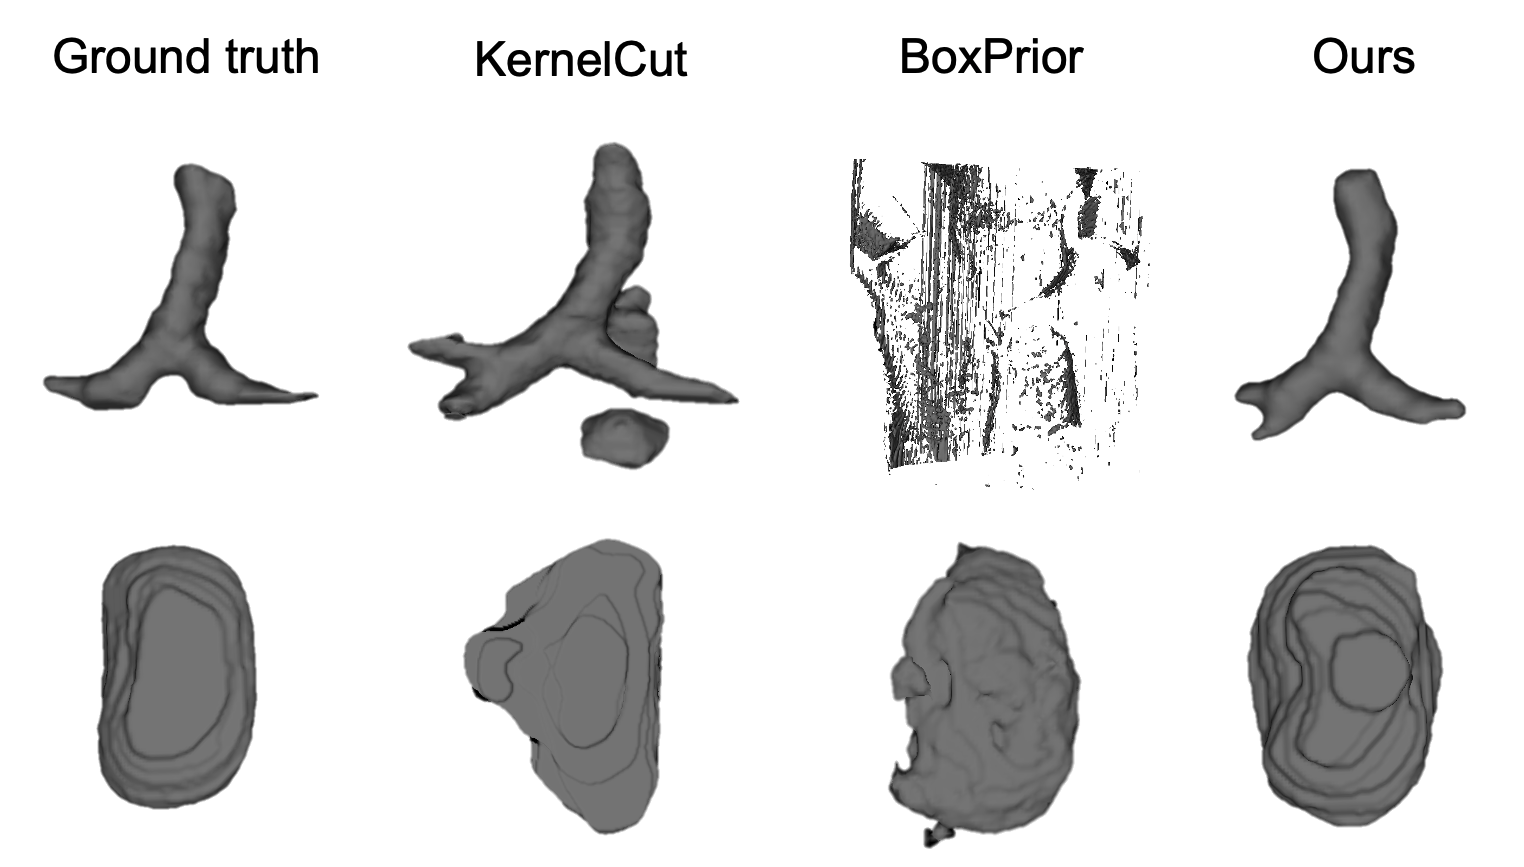
\includegraphics[width=1.0\textwidth]{img/c3/final_vis4.png}
        \bicaption{不同方法在两个数据集上的可视化结果,实验设定是 30\% 的弱标注比例。第一行:气管的三维分割,第二行:前列腺的三维分割。}
        {Qualitative results on three datasets with 30\% labeled slices. First row: trachea segmentation. Second row: prostate segmentation.}
        \label{fig:vis}
    \end{figure*}


\subsection{消融实验} \label{sec:ablate}

我们对所提出的弱监督分割框架做了详细的消融实验,包括表~\ref{tab:ablate1}在模型方法的实验,表~\ref{tab:ablate2}在弱标签的对比,以及表~\ref{tab:ablate_loss}在损失函数项的实验。接下来我们一一分析。

\paragraph{形状先验}
形状去噪网络使用自学习的形状先验进行形状改进。表~\ref{tab:ablate1}中的 CRF 代表用 DenseCRF 代替形状去噪网络,这使最终性能下降2\%-3\%。此外,DenseCRF 在三维体积图像上的后处理需要大约 3.50 秒,而我们的形状去噪网络的推理过程只需要 0.02 秒。更进一步,去除形状去噪网络,即去除公式~\ref{eq1}和公式~\ref{eq2} 中的 $\mathbf{M}_d$ 和 $(1-\mathbf{M}_d)$,会导致性能下降4\%-5\%。
\paragraph{迭代学习}
迭代学习把学习到的形状先验引入训练过程,以迭代改进我们的分割模型。如果没有迭代学习策略,模型的性能会下降约9\%。
\paragraph{弱标签}
我们将混合式标签与不同类型的涂鸦式标签和边界框标签进行比较。表~\ref{tab:ablate2}的结果表明,混合式标签的结果相比其他标签高出相当大的差距。这表明在更多的形状上下文下,混合式标签以相同的成本含有比其他标签更多的信息量。实验中的所有的涂鸦式标签与我们的混合标签的前景标签是一样的。
表中的 Scribble* 表示将我们的宽松边界框作为背景涂鸦,Scribble(20-50)也采用松散边界框,但与紧致框有20-50像素的较大距离,Scribble(dilation)表示真实物体边缘向外膨胀产生的涂鸦。Scribble*直接来自于我们的混合式标签,与其他的 Scribble 变体相比,它取得了最好的结果,这表明在相同的标签成本下,它可能是信息最丰富的 Scribble 形式。
对于紧致边界框标签,我们首先用 GrabCut 从标注的切片中生成前景和背景标签,并在我们的方法中使用它们作为模型学习的弱标签。
\paragraph{损失函数}
我们还研究了公式~\ref{eq3}中两个损失函数项对模型训练的影响。如表~\ref{tab:ablate_loss}所示。只使用伪标签进行迭代训练,呈现出明显优于基线10\%以上的表现。同时使用弱标签和伪标签,我们的方法可以进一步提高性能1\%-2\%。

\begin{table}[t!]
    \centering    
    \bicaption{对模型组成部分的消融实验。实验在气管分割上进行,以每次消融一个变量的方式进行。}
    {Ablation study on our model components. We conduct experiments in a drop-one-out manner.}
    \begin{tabular}[t]{c c c|c c c}
        \toprule
        \multirow{2}{*}{Method} & \multirow{2}{*}{Shape prior} & \multirow{2}{*}{Iterative}  & \multicolumn{3}{c}{Trachea (Val)} \\ %\cline{4-6}
        &                       &              & 50\% & 30\% & 10\%                 \\ \midrule
        Ours      & $\checkmark$  & $\checkmark$      & \textbf{83.45} & \textbf{83.18} & \textbf{83.18} \\ %\\
        %            \midrule
        & CRF      & $\checkmark$      & 81.08 & 80.48 & 80.36 \\
        & --            & $\checkmark$      & 78.97 & 78.59 & 78.11 \\ %\hline
        & $\checkmark$  & --                & 74.91 & 74.80 & 74.17 \\
        Baseline      & --            & --                          & 69.17 & 68.39 & 62.50 \\
        \bottomrule 
    \end{tabular}
    \label{tab:ablate1}
\end{table}

\begin{table}[t!]
    \centering    
    \bicaption{对弱标注方法的对比研究。本文提出的混合式标签被用来和不同类型的涂鸦式标签以及边界框标签比较。}
    {Ablation study on annotations. We compare our hybrid label to different types of scribbles and box.}
    \begin{tabular}[t]{c c|c c c}
        \toprule
        \multirow{2}{*}{Method} & \multirow{2}{*}{Annotation} & \multicolumn{3}{c}{Trachea (Val)} \\ %\cline{4-6}
        &                        & 50\% & 30\% & 10\%                 \\ \midrule            
        Ours &   Hybrid  & \textbf{83.45} & \textbf{83.18} & \textbf{83.18} \\
        %            \midrule
        & Scribble*      & 83.05  & 82.75 & 81.63 \\
        & Scribble (20-50)      & 78.91 & 75.80 & 75.45 \\ %\hline  \hline
        & Scribble (dilation)      & 78.86 & 77.99 & 76.60 \\
        & Box                   & 82.25 & 81.70 & 80.60 \\
        % Baseline    & Scribble      & --            & --                          & 68.35 & 65.68 & 62.98 \\   \hline  \hline
        %             & Box     & 82.95 & 81.84 & 79.59 \\ 
        \bottomrule 
    \end{tabular}
    \label{tab:ablate2}
\end{table}

\begin{table}[t!]
	\centering
	\bicaption{对我们方法中的两项损失的消融实验。}
    {Ablation study on two loss terms of our method.}
	\label{tab:ablate_loss}        
	% \resizebox{0.6\textwidth}{!}{
		\begin{tabular}[t]{c c c|c c c}
			\toprule
			\multirow{2}{*}{Method} & \multirow{2}{*}{Weak label} & \multirow{2}{*}{Pseudo label}  & \multicolumn{3}{c}{Trachea (Val)} \\ %\cline{4-6}
			&                       &              & 50\% & 30\% & 10\%                 \\ \midrule
			Baseline  & $\checkmark$  & --      & 69.17 & 68.39 & 62.50 \\
			& --      & $\checkmark$  & 81.89 & 81.57 & 81.14 \\
			Ours      & $\checkmark$  & $\checkmark$      & \textbf{83.45} & \textbf{83.18} & \textbf{83.18} \\
			\bottomrule 
		\end{tabular}
	% }
\end{table}

\subsection{拓展讨论} \label{sec:extension}

\paragraph{网络结构}
对于语义分割网络,我们遵循 nnU-Net~\citep{isensee2019automated} 的设计原则使用 3D U-Net 网络结构,包括一个编码器和一个解码器。
我们对每个数据集的详细网络结构见图~\ref{fig:s_net1, fig:s_net2, fig:s_net3},相应的网络配置见表~\ref{tab:net_params}。
编码器和解码器都由四层或五层组成,取决于输入图像的分辨率。每个计算块由三种操作顺序组成,依次为卷积层(conv)- 实例归一化(instance norm)- 泄漏整流线性单元(leaky ReLU)。每层包含两个计算块,其不改变特征空间分辨率。我们用步幅卷积(strided convolution)实现下采样,用转置卷积(transposed convolution)实现上采样。对于形状去噪网络,我们采用了语义分割网络相同的结构,但其具有独立的参数。

    \begin{figure*}[tbp]
        \centering 
        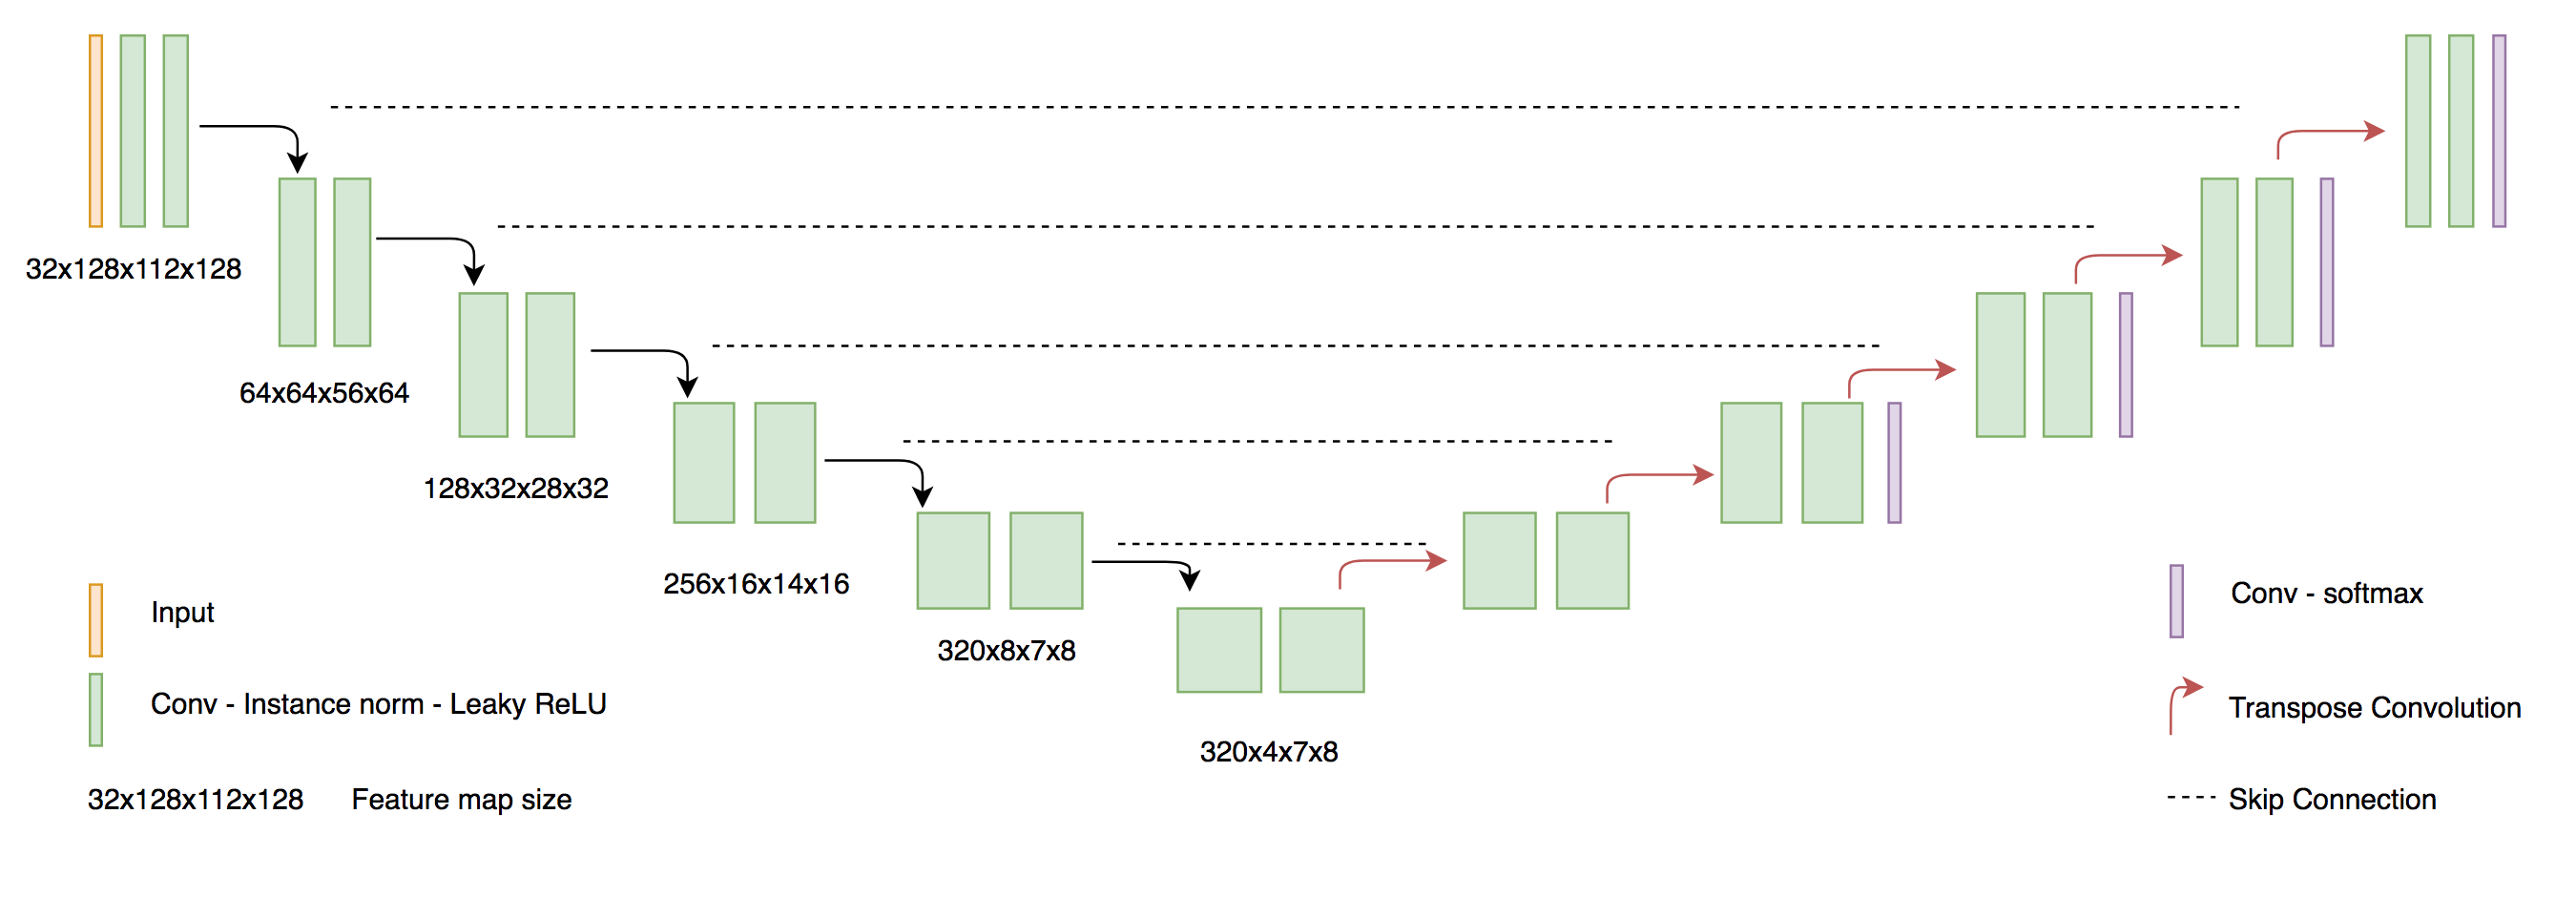
\includegraphics[width=1.0\textwidth]{img/c3/s_net.png}
        \bicaption{气管数据集的网络结构}
        {Network architecture for trachea dataset.}
        \label{fig:s_net1}
    \end{figure*}


    \begin{figure*}[tbp]
        \centering 
        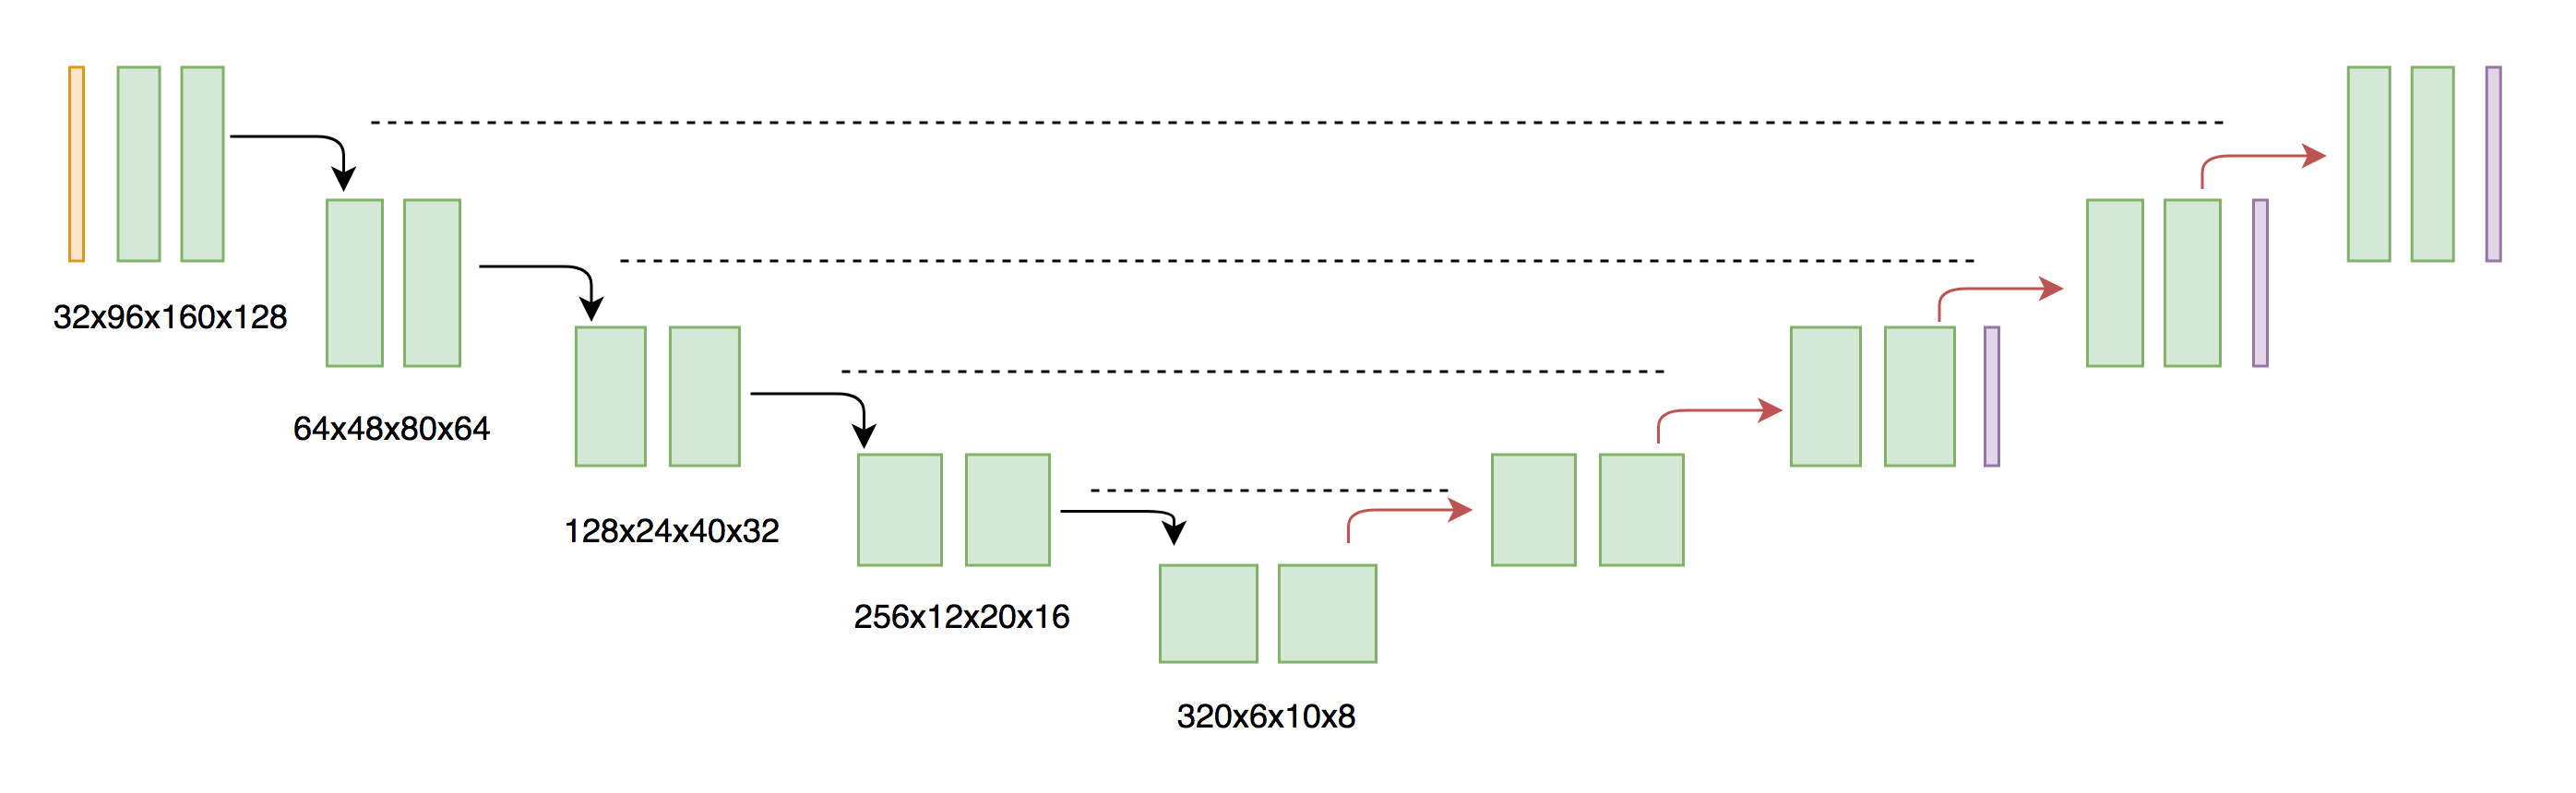
\includegraphics[width=1.0\textwidth]{img/c3/s_net2.png}
        \bicaption{左心房数据集的网络结构}
        {Network architecture for left atrium dataset.}
        \label{fig:s_net2}
    \end{figure*}


    \begin{figure*}[tbp]
        \centering 
        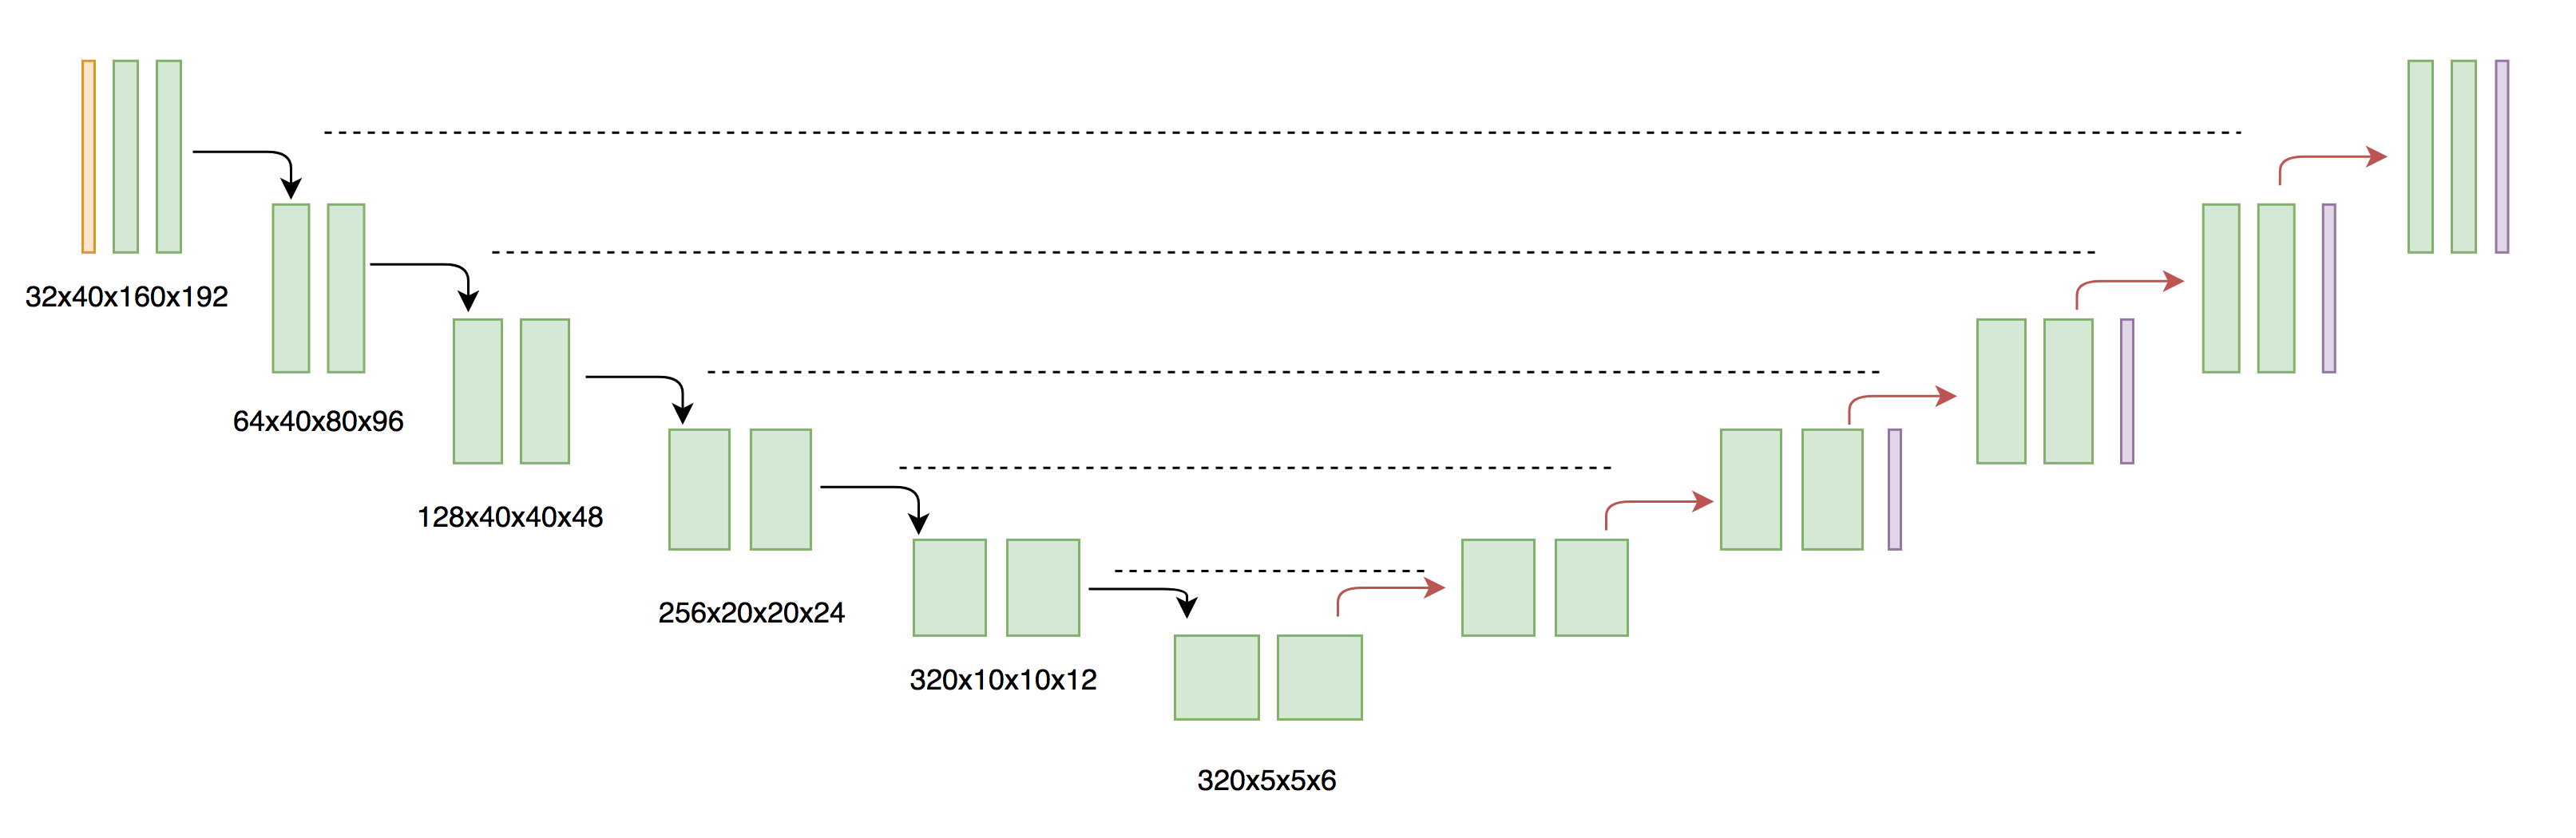
\includegraphics[width=1.0\textwidth]{img/c3/s_net3.png}
        \bicaption{前列腺数据集的网络结构}
        {Network architecture for prostate dataset.}
        \label{fig:s_net2}
    \end{figure*}

    \begin{table*}[t!]
	\centering
	\bicaption{用于气管、左心房和前列腺数据集的网络配置。}
    {Network configurations for trachea, left atrium and prostate datasets.}
	\label{tab:net_params}        
	\resizebox{\textwidth}{!}{
		\begin{tabular}{c| c c c}
			\toprule
			& Trachea & Left Atrium & Prostate  \\ \midrule
			Input spacing (mm)     & $2.50\times1.63\times1.63$ & $0.63\times1.33\times1.33$  & $2.20\times0.72\times0.72$  \\
			Input resolution & $128\times112\times128$ & $96\times160\times128$  & $40\times160\times192$  \\
			Pooling strides & $[[2,2,2], [2,2,2], [2,2,2], [2,2,2], [2,1,1]]$ & $[[2,2,2], [2,2,2], [2,2,2], [2,2,2]]$  & $[[1,2,2], [1,2,2], [2,2,2], [2,2,2], [2,2,2]]$  \\
			Convolution kernel sizes & $[[3,3,3], [3,3,3], [3,3,3], [3,3,3], [3,3,3], [3,1,1]]$ & $[[3,3,3], [3,3,3], [3,3,3], [3,3,3], [3,3,3]]$  & $[[1,3,3], [1,3,3], [3,3,3], [3,3,3], [3,3,3], [3,3,3]]$  \\
			\bottomrule
		\end{tabular}
	}
\end{table*}


\paragraph{形状去噪网络的分析}
这一部分我们进一步讨论形状去噪网络。我们的形状去噪网络设计是基于这样的假设:在弱标签上训练的语义分割网络能够提供初始掩膜,这为形状去噪网络提供了良好的起点。实验中发现,训练集中的一些实例“看起来”比其他实例具有更好的质量,即具有干净和完整的形状。然后,我们通过计算每个预测掩膜的前景像素的平均概率作为置信度,发现具有最高置信度的掩膜一般具有最好的形状质量。因此,我们把语义分割网络预测的具有最高可信度的掩膜,视作可获得的正确形状,来训练形状去噪网络。训练完成后,形状去噪网络之后不再更新,主要是因为最初选择的掩膜在形状上有足够好的质量,并且实验探索发现,我们发现之后用新的形状更新形状去噪网络,并没有带来进一步的改进。

需要注意的是,在模型训练或推理阶段,我们没有使用任何训练数据的真实掩模。但我们可以追溯验证所选掩膜是否具有良好的质量,这可以通过计算所选掩膜相比真实掩膜的 dice 系数来实现。以气管上的30\%弱标注比例为例,我们所选形状的 dice 系数是87.89\%。在我们的整个模型训练完成后,它的 dice 系数提高到了 90.62\%,这在形状层面上改变微小。

我们在表~\ref{tab:ablation_aug}中进一步分析了形状去噪网络的设计。我们提出的所有增强操作都有助于改善形状去噪网络对噪音和错误的消除,特别是膨胀操作,使性能提高了3.83\%。此外,我们还使用具有不同置信度的预测形状实例来训练,结果对比表明,置信度最高的实例提供了最好的形状先验信息,而我们的设计对形状选择标准也很鲁棒。即使选择一个置信度相对较低的形状预测(第7行,实例排序为30),仍然提供了对基线的改进,表明我们的噪声增强和去噪学习能够在缺少高质量形状表示时也表现良好。

对初始化训练的语义分割网络的观察中,我们发现数据集中的一类器官通常具有非常相似的形状。其主要变化可以通过一些适度的空间变换来捕捉,包括平移、旋转和缩放等。
因此,我们在单个选定的形状上应用随机空间变换来增强,以形成形状分布。实验中我们发现使用一个单一的形状,配合增强方法,是足以解决目标任务的。我们进行了以下实验:分别选择第1个、前3个或前5个具有最高可信度的形状来训练形状去噪网络,结果表明使用更多的形状没有带来进一步的增益。对于形状变化较大的体积分割,我们的方法有可能扩展到多形状的学习,比如,采用标准的聚类方法来获得几类形状模板,为每类形状训练一个独立的自动编码器,并通过基于相似性的投票来产生最终结果。

    % Table: ablation sdn
    \begin{table}[t!]
        \centering
        \bicaption{对形状去噪网络的分析,该实验在气管数据集的验证集上进行,弱标签比例为 30\%。我们以逐个增加的方式展示每个增强操作的贡献。此外,我们还展示了使用不同样本作为形状表示进行训练的效果。实例排序(case rank)表示所选形状表示的置信度排序。}
        {Analysis of our SDN on the validation split of trachea dataset with 30\% labeled slices. We present the contribution of each augmentation operation in an incremental manner. Moreover, we also show the effect of using different cases as our shape representation for training. Case rank denotes the confidence rank of the selected shape representation.}
        \label{tab:ablation_aug}        
        % \resizebox{0.65\textwidth}{!}{
            \begin{tabular}{c c c c c c c}
                \toprule
                & Case rank & Closing     & Dilation     & Extension      & Dice [\%]  \\ \midrule
                Baseline & 1 & --              & --                & --                & 68.39        \\
                & 1 & $\checkmark$    & --                & --                & 69.19         \\ %\hline
                & 1 & $\checkmark$    & $\checkmark$      & --                & 73.02        \\ %\hline
                Our SDN  & 1 & $\checkmark$    & $\checkmark$      & $\checkmark$      & \textbf{74.80}             \\ \midrule
                & 2 & $\checkmark$    & $\checkmark$      & $\checkmark$      & 74.62             \\ 
                & 15 & $\checkmark$    & $\checkmark$      & $\checkmark$      & 74.05             \\ 
                & 30 & $\checkmark$    & $\checkmark$      & $\checkmark$      & 72.62             \\ 
                \midrule
                & Top 1-3 & $\checkmark$    & $\checkmark$      & $\checkmark$      & 74.08             \\
                & Top 1-5 & $\checkmark$    & $\checkmark$      & $\checkmark$      & 73.98             \\
                \bottomrule
            \end{tabular}
        % }
    \end{table}






\section{本章小结}
在本章中,我们为基于弱标签的弱监督语义分割任务开发了一种新的方法,并为弱监督的三维图像提出了一种稀疏的注释方案。我们提出一种自学习的形状去噪网络,它能够将分割后的掩模改进为更好的形状。并且我们通过在迭代更新模型中引入学到的形状先验带来更高的性能。此外,我们的稀疏标注方案在相同的标注成本下提供了比其他弱标签更多的信息。在两个具有不同形状属性的基准数据集的实验评估表明,我们所提的弱监督分割框架稳定地超过了其他利用不同弱标签的近期工作。
\chapter{基于置信度的语义匹配}

\section{章节概述}
简介
\section{问题设定和概述}
本文研究内容
\section{方法}
本文研究内容
\subsection{空间上下文编码器}
考虑空间上下文的特征表达
\subsection{相关网络}
动态混合
\subsection{动态混合网络}
置信度估计


\chapter{总结与展望}

\section{总结}
本文中,为了解决医学图像中的语义分割所需训练标签的高成本与难获取的问题,我们探索了弱监督语义分割的两个方向:基于弱标签和基于噪声标签的学习。
基于弱标签的语义分割只需要粗标注形式,我们为该任务提出了一种结合物体形状先验的弱分割模型与学习策略。我们的方法在模型训练与预测中很好地利用形状先验,来弥补标签不足带来的分割性能下降。由于缺少完整的物体形状,我们利用弱标签,设计了一种自学习的形状表示,其中包括形状表示的选取、形状增强方法和形状去噪模型。语义分割模型和形状模型的结合,大大提高了训练过程和最终预测的效果。迭代学习的策略,使得弱监督分割模型性能逐步提高并稳定收敛。
此外,我们设计了高效的稀疏弱标注策略,包含选择标注和混合式标签,通过利用空间连续性和整体性,大大降低了标注成本,而尽可能保留弱标签的丰富信息量。
我们在两个不同的数据集上(气管和前列腺)的实验结果表明,所提出的方法在多个弱标注设定下都取得了最高的性能,并且表现出很强的鲁棒性。在可视化结果的对比上,我们的分割结果具有更干净完整的形状,证明了我们方法对物体形状的充分捕捉,以及形状先验在弱监督语义分割中的重要作用。

基于噪声标签的语义分割的核心问题,是充分利用正确标签,而减少错误标签对训练的干扰。为此,我们利用图像的结构先验和像素标签的相关性,提出一种结合超像素表示的鲁棒学习的策略。
超像素表示能使我们在分割标签上施加结构约束,并且尽可能保留物体的边缘信息。而在模型学习中基于超像素表示,我们可以更准确地选择可靠的正确标签用以训练,并纠正不可靠的标签。在训练策略上,我们提出了有噪声感知的网络更新和标签更新交替进行的迭代学习,充分利用了标签的有效信息并不断更新改进。
我们的方法在两个数据集的四种类别上进行实验,结果表明我们方法超越之前方法的优异性能,并保持了训练的稳定收敛。多种噪声水平设定下的数值变化表明,我们的方法具有较强的鲁棒性和泛化性能。另外,我们的预测结果更接近真实完整的物体边缘。

\section{展望}
以上两个方向的探索过程中,我们发现了一些进一步的问题值得研究。

在基于弱标签的语义分割中,我们也发现了一些误差较大的案例,如图~\ref{fig:failure}所示。它们表现为不完整的或过多的预测掩膜,即使其输入图像在像素强度或边缘都比较明显。
这主要是因为我们的模型是在弱标签上训练,而没有在训练中探索物体边缘信息或约束。这样的问题,可以考虑在模型中加入图像的低阶特征,比如边缘特征或超像素等,来进一步改善。
    \begin{figure}[tbp]
        \centering 
        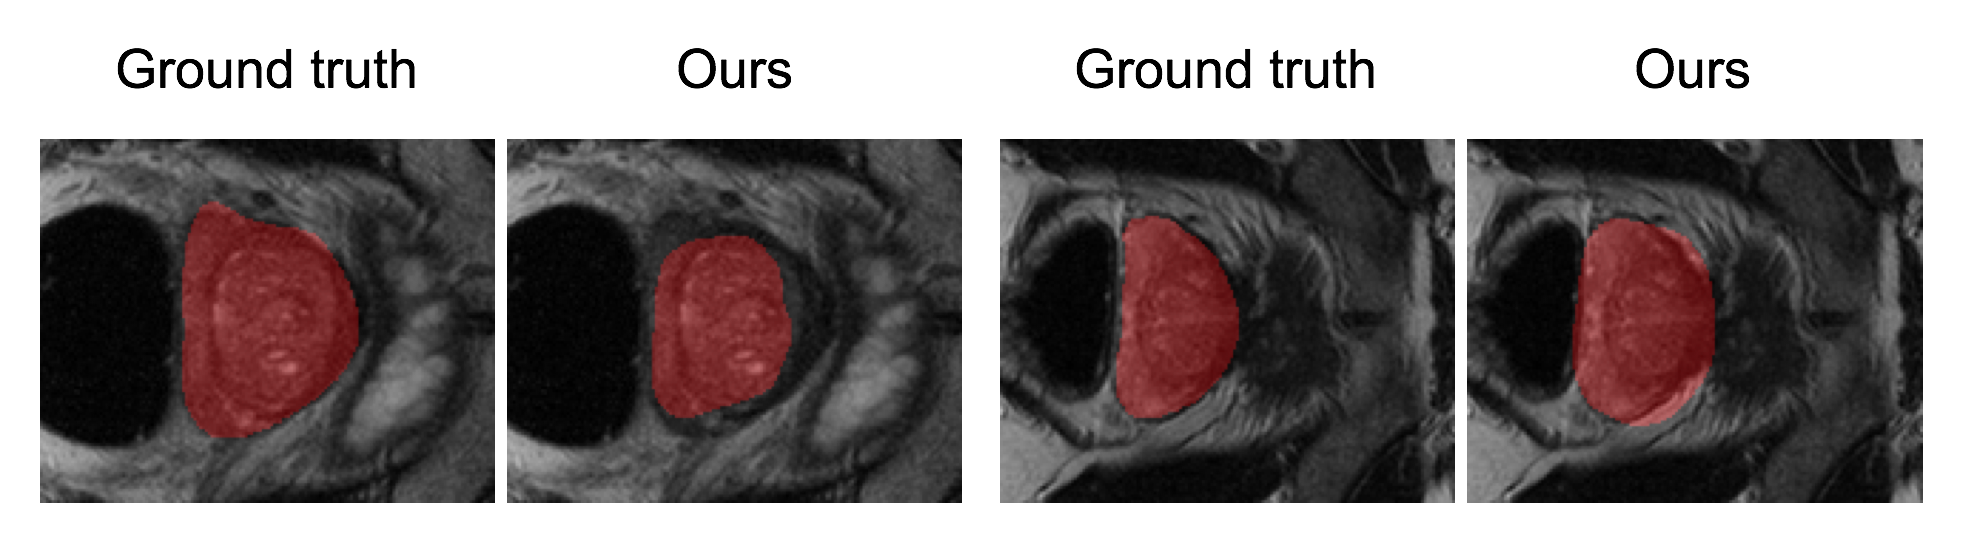
\includegraphics[width=1.0\textwidth]{img/c3/failure.png}
        \bicaption{两个在前列腺数据集的失败的预测案例。}
        {Two failure cases on prostate dataset.}
        \label{fig:failure}
    \end{figure}

另外,由于多数的医学图像的目标分割器官都有较大的相似性,我们的方法实际上是捕捉了一类相近的形状表示。但真实世界中也有很多类别的物体具有较大的形状差异,当它们无法用一类形状来表示,而呈现出多类或者层次结构的形状时,我们的方法就需要进行拓展。具体而高效的形状模型需要更多探索。更进一步,现有的形状模型拥有大量的参数,训练需要大量时间而部署也需要较大内存,能否降低形状模型的复杂度,或者将其与语义分割模型深度结合,是很有前景的方向。

在基于噪声标签的语义分割中,超像素的质量和真实噪声数据集值得进一步关注。
我们的基于超像素表示的鲁棒学习方法被证明是有效的,并且具有较好的鲁棒性和泛化性。但是,超像素的生成质量依旧有一些误差,这些误差一定程度上限制了方法效果的进一步提升。
现有的离线生成方法(如 SLIC)改进空间不大,如何自适应地生成更准确的超像素,或者更广泛的,感知分组,具有十分重要的意义。
在更广泛的应用场景,比如同一图像中不同尺寸的目标物体,如何设计高质量的基于图像结构先验的表示方法,是需要深入探索的。

在数据集层面,由于缺少公开的真实噪声标签的数据集,我们使用模拟的标签噪声作为替代。虽然探索了膨胀、腐蚀等形态学和仿射变换等噪声模式,真实的标签噪声可能呈现更多样更细节的变化。为了所提方法的可用性和泛化性,探索真实世界的噪声标签处理是一个重要的课题。只是建立这样一个数据集需要非同寻常的努力,因此我们把它留给未来的工作。
\makebiblio
\backmatter
\ifgraduate
\begin{resume}
李帅霖,山西运城人,上海科技大学 2018 级硕士研究生。
\end{resume}

\begin{education}
2018.9 - 至今:      \quad 硕士 \quad 上海科技大学 \quad 计算机科学与技术

2014.9 - 2018.6     \quad 学士 \quad 南方科技大学 \quad 计算机科学与技术
\end{education}

\begin{publications}
%   论文发表…… (非匿名环境)
\begin{enumerate}
    \item Li, Shuailin, Zhitong Gao, and Xuming He. "Superpixel-Guided Iterative Learning from Noisy Labels for Medical Image Segmentation." International Conference on Medical Image Computing and Computer-Assisted Intervention (MICCAI). Springer, Cham, 2021.
    \item He, Qian, Shuailin Li, and Xuming He. "Weakly Supervised Volumetric Segmentation via Self-taught Shape Denoising Model." Medical Imaging with Deep Learning (MIDL). 2021.
    \item Li, Shuailin, Chuyu Zhang, and Xuming He. "Shape-aware semi-supervised 3d semantic segmentation for medical images." International Conference on Medical Image Computing and Computer-Assisted Intervention (MICCAI). Springer, Cham, 2020.
\end{enumerate}

\end{publications}

\begin{publications*}
%   论文发表…… (匿名环境)
\end{publications*}

% \begin{patterns}
%   专利申请或授权记录…… (非匿名环境)
% \end{patterns}

% \begin{patterns*}
%   专利申请或授权记录…… (匿名环境)
% \end{patterns*}

% \begin{projects}
%   个人参与的科研项目、获奖情况…… (仅非匿名环境显示)
% \end{projects}
\fi


\begin{acknowledgement}
岁月不居,时节如流,研究生生涯踏入尾声。
这三年多的时间里,有初入研究的懵懂,有踌躇不前的苦闷,有好高骛远的落差,也有不达不休的决心,有柳暗花明的欣喜,有再接再厉的勇气。
人在环境中成长,我很感谢自己所处的这个环境。导师何旭明教授给予了专业而深入的科研训练,使我从懵然无知的新人成长为略有积累的研究生。实验室的同学们,使我在良好的研究氛围中不断借鉴学习。上科大的丰富资源,提供了全面而重要的支持。
我向这三年多来遇到的每一个人致谢,他们或是博学亲切的教授,或是乐于助人的同学,或是默默付出的宿管,或是关护温和的前辈。
最后,感谢亲人们的关心、支持与鼓励,感谢与我探讨过诸多问题的朋友们,他们都使我受益匪浅,乐观应对生活这一课题。
回望身后,所历种种,但曙光初露,这个故事,才刚刚开始呢。

\end{acknowledgement}

\end{document}
